\documentclass[11pt]{article}

% basic packages
\usepackage[margin=1in]{geometry}
\usepackage[pdftex]{graphicx}
\usepackage{amsmath,amssymb,amsthm}
\usepackage{custom}      % loads everything else (see custom.sty)

\renewcommand\qedsymbol{$\blacksquare$}

% page formatting
\usepackage{fancyhdr}
\pagestyle{fancy}

\renewcommand{\sectionmark}[1]{\markright{\textsf{\arabic{section}. #1}}}
\renewcommand{\subsectionmark}[1]{}
\lhead{\textbf{\thepage} \ \ \nouppercase{\rightmark}}
\chead{}
\rhead{}
\lfoot{}
\cfoot{}
\rfoot{}
\setlength{\headheight}{14pt}

\linespread{1.03}
\setlength{\parindent}{0.2in}
\setcounter{secnumdepth}{2}
\setcounter{tocdepth}{2}

\graphicspath{{figures/}}

\begin{document}

% --- title page ---
\thispagestyle{empty}
\bigskip
\vspace{0.1cm}

\begin{center}
{\fontsize{30}{30}\selectfont\bfseries\sffamily CS3230\\[0.4em]
Design and Analysis of Algorithms}\\
\vspace{18pt}
{\fontsize{14}{14}\selectfont\rmfamily Open-Book Examination Notes}\\
\vspace{18pt}
{\fontsize{14}{14}\selectfont\rmfamily Donald Kong}\\
\vspace{6pt}
{\fontsize{12}{12}\selectfont\ttfamily dkkl1137@gmail.com}\\
\vspace{18pt}
{\fontsize{11}{11}\selectfont\rmfamily S2 AY2025/26}
\end{center}

\vspace{1cm}

% --- top-level table of contents ---
\microtoc%
\newpage

% --- front matter (formula companion + problem-solving checklist) ---
% Front matter: quick reference and problem-solving checklist.
\section*{Quick reference}
\addcontentsline{toc}{section}{Quick reference}
\label{sec:quickref}

\paragraph{Logs and exponentials.}
\begin{itemize}
  \item $a^{\log_b c} = c^{\log_b a}$
  \item $\log_b(xy) = \log_b x + \log_b y$,\quad $\log_b(x^k) = k \log_b x$
  \item $e^x \ge 1 + x$ for all $x$;\quad $\ln(1 + x) \le x$ for $x > -1$
\end{itemize}

\paragraph{Series.}
\begin{itemize}
  \item Arithmetic: $\sum_{i=1}^n i = n(n+1)/2$
  \item Geometric: $\sum_{i=0}^{n-1} r^i = (r^n - 1)/(r - 1)$ for $r \ne 1$;\quad
        $\sum_{i=0}^\infty r^i = 1/(1 - r)$ for $|r| < 1$
  \item Harmonic: $H_n = \sum_{i=1}^n 1/i = \ln n + \Theta(1)$
\end{itemize}

\paragraph{Stirling's approximation.}
$n! = \sqrt{2\pi n}\, (n/e)^n (1 + \Theta(1/n))$;\quad
in particular $\log_2(n!) = n \log_2 n - n \log_2 e + \Theta(\log n)$.

\paragraph{Probability.}
\begin{itemize}
  \item Linearity: $\expec[X + Y] = \expec[X] + \expec[Y]$ (always)
  \item Markov: $\prob[X \ge a] \le \expec[X]/a$ for $X \ge 0$, $a > 0$
  \item Chebyshev: $\prob\bigl[\,|X - \expec[X]| \ge a\,\bigr] \le \mathrm{Var}(X)/a^2$
  \item Union bound: $\prob\bigl[\bigcup_i A_i\bigr] \le \sum_i \prob[A_i]$
\end{itemize}

\paragraph{Master Theorem.}
For $T(n) = a T(n/b) + f(n)$ with $a \ge 1$, $b > 1$, let $c^* = \log_b a$:
\begin{itemize}
  \item Case 1: $f(n) = O(n^{c^* - \varepsilon})$ for some $\varepsilon > 0$ \(\Rightarrow\) $T(n) = \Theta(n^{c^*})$
  \item Case 2: $f(n) = \Theta(n^{c^*})$ \(\Rightarrow\) $T(n) = \Theta(n^{c^*} \log n)$
  \item Case 3: $f(n) = \Omega(n^{c^* + \varepsilon})$ and $af(n/b) \le k f(n)$ for some $k < 1$ and large $n$ \(\Rightarrow\) $T(n) = \Theta(f(n))$
\end{itemize}

\section*{Solving an algorithm problem: moves to consider}
\addcontentsline{toc}{section}{Solving an algorithm problem: moves to consider}
\label{sec:checklist}

\textbf{For an algorithm-design problem, try in order:}
\begin{enumerate}
  \item \textbf{Greedy} (\cref{sec:greedy}). Identify the locally optimal choice; attempt an exchange argument. Often the intended solution; cheap to try first.
  \item \textbf{Divide and conquer} (\cref{sec:dnc}). Look for a way to split the input into independent subproblems of similar shape; analyse via Master Theorem (\cref{sec:recurrences}).
  \item \textbf{Dynamic programming} (\cref{sec:dp}). Identify subproblems and a recurrence; check overlap; tabulate. Time = (state space) $\times$ (per-transition cost).
  \item \textbf{Reduction} (\cref{sec:reductions}). Reduce to a known polynomial-time problem (e.g., max-flow, shortest paths) -- or, if intractability is suspected, reduce a known NP-hard problem to it (\cref{sec:npc}).
  \item \textbf{Randomisation} (\cref{sec:randomised}). When deterministic structure is hard to exploit, try a Las Vegas or Monte Carlo strategy; analyse via linearity of expectation.
\end{enumerate}

\textbf{For a correctness proof:} state a loop invariant or inductive hypothesis explicitly; show init / maintenance / termination (\cref{sec:correctness}).

\textbf{For a complexity analysis:} write down the recurrence; identify $a$, $b$, $f(n)$; apply the Master Theorem case-decision tree (\cref{fig:mt_cases}).

\textbf{For an NP-hardness proof:} pick a known NP-complete problem (\cref{sec:npc}) and construct a polynomial-time mapping reduction to the target. State the mapping and prove correctness in both directions.

\textbf{For a data-structure analysis:} if costs vary across operations but the total over a sequence is bounded, this is amortised analysis -- pick aggregate / accounting / potential and apply (\cref{sec:amortised}).

\newpage

% --- Part I: Foundations ---
\part{Foundations}
% Chapter 1: Mathematical Preliminaries.
\section{Mathematical Preliminaries}
\label{sec:math}

Algorithm analysis throughout these notes draws on three small toolkits: discrete probability, elementary asymptotic identities, and a handful of closed-form sums. This chapter fixes notation and collects the working set used throughout the remainder of the notes.

\subsection{Notation and basic concepts}

A \emph{probability space}\index{probability space}\index{sample space}\index{event} consists of a finite sample space $S$ and a probability measure $\prob$ assigning to each event $A \subseteq S$ a value $\prob(A) \in [0,1]$, with $\prob(S) = 1$ and $\prob(A \cup B) = \prob(A) + \prob(B)$ for disjoint $A, B$. Two events are \emph{independent} if $\prob(A \cap B) = \prob(A)\prob(B)$. A \emph{random variable}\index{random variable} $X$ is a function $X : S \to \reals$; its \emph{expectation}\index{expectation} is $\expec[X] = \sum_x x \cdot \prob(X = x)$. The \emph{indicator}\index{indicator variable} $\indic_A$ of an event $A$ is the random variable taking value $1$ when $A$ occurs and $0$ otherwise, so that $\expec[\indic_A] = \prob(A)$. The \emph{variance}\index{variance} of $X$ with mean $\mu$ is $\Var[X] = \expec[(X-\mu)^2] = \expec[X^2] - \mu^2$, and the \emph{standard deviation}\index{standard deviation} is $\sigma_X = \sqrt{\Var[X]}$. Variance scales as $\Var[aX] = a^2 \Var[X]$ and is additive over independent summands: $\Var[\sum_i X_i] = \sum_i \Var[X_i]$ if the $X_i$ are pairwise independent.

\subsection{Key results}

\begin{theorem}[Linearity of expectation]
\label{thm:linearity}
For any random variables $X_1, \dots, X_n$ on a common probability space and any constants $a_1, \dots, a_n \in \reals$,
\[
  \expec\!\left[\sum_{i=1}^n a_i X_i\right] \;=\; \sum_{i=1}^n a_i\, \expec[X_i].
\]
The $X_i$ need \emph{not} be independent.
\end{theorem}

\begin{theorem}[Markov's inequality]
\label{thm:markov}
Let $X$ be a non-negative random variable. Then for every $t > 0$,
\[
  \prob(X \ge t) \;\le\; \frac{\expec[X]}{t}.
\]
\end{theorem}

\begin{remark}
Markov requires $X \ge 0$; applied to a possibly-negative variable, the bound fails. It bounds only the upper tail and is informative only when $t > \expec[X]$ (otherwise $\expec[X]/t \ge 1$). For variables that may be negative, apply Markov to $|X|$, $X^2$, or $X - \min$.
\end{remark}

\begin{theorem}[Chebyshev's inequality]
\label{thm:chebyshev}
Let $X$ be a random variable with finite mean $\mu = \expec[X]$ and finite variance $\sigma^2 = \Var[X]$. Then for every $t > 0$,
\[
  \prob\bigl(|X - \mu| \ge t\bigr) \;\le\; \frac{\sigma^2}{t^2}.
\]
\end{theorem}

\begin{remark}
The denominator is $t^2$, not $t$: a frequent slip is to write $\Var[X]/t$. Equivalently, $\prob(|X - \mu| \ge k\sigma) \le 1/k^2$.
\end{remark}

\begin{theorem}[Union bound]
\label{thm:union_bound}
For any events $A_1, A_2, \dots, A_n$ on a common probability space,
\[
  \prob\!\left(\bigcup_{i=1}^n A_i\right) \;\le\; \sum_{i=1}^n \prob(A_i).
\]
\end{theorem}

\begin{remark}
The union bound is loose but free, and is often tight enough. For highly correlated or numerous events, an inclusion--exclusion or second-moment argument may be sharper.
\end{remark}

\begin{remark}[Why these four are the workhorses]
Linearity (which does not require independence) converts expected-count problems into sums of indicator probabilities and underpins average-case running-time analyses. Markov turns a single moment bound into a tail bound; Chebyshev sharpens this when the second moment is available; the union bound concludes ``with high probability nothing bad happens'' from per-event failure probabilities.
\end{remark}

\subsection{Reference identities}

The following identities are used without proof throughout the notes; they are collected here for reference.

\paragraph{Exponentials and logarithms.} For all $a, b, c > 0$ and real $m, n, x$:
\begin{align*}
  a^m a^n &= a^{m+n}, & (a^m)^n &= a^{mn}, & a^{-1} &= 1/a, \\
  e^x &\ge 1 + x, & \ln x &\le x - 1\ \text{for } x > 0, & a &= b^{\log_b a}, \\
  \log_c(ab) &= \log_c a + \log_c b, & \log_b(a^c) &= c\log_b a, & \log_b a &= \frac{\log_c a}{\log_c b} = \frac{1}{\log_a b}, \\
  a^{\log_b c} &= c^{\log_b a}.
\end{align*}
The base of a logarithm is irrelevant inside $\Theta(\cdot)$ since $\log_a n = \Theta(\log_b n)$ for any constant bases $a, b > 1$. Bases of \emph{exponentials} are not asymptotically interchangeable: $4^n \notin \Theta(2^n)$.

\paragraph{Arithmetic and geometric series.}
\begin{align*}
  \sum_{i=1}^{n} i &= \frac{n(n+1)}{2}, &
  \sum_{i=1}^{n} i^2 &= \frac{n(n+1)(2n+1)}{6}, &
  \sum_{i=1}^{n} i^k &= \frac{n^{k+1}}{k+1} + O(n^k), \\
  \sum_{i=0}^{n} r^i &= \frac{1 - r^{n+1}}{1 - r}\ (r \ne 1), &
  \sum_{i=0}^{\infty} r^i &= \frac{1}{1 - r}\ (|r| < 1), &
  \sum_{i=0}^{\infty} i\, r^i &= \frac{r}{(1-r)^2}\ (|r| < 1).
\end{align*}

\paragraph{Harmonic numbers.} The $n$-th harmonic number is $H_n = \sum_{i=1}^{n} 1/i$. Comparing with $\int_1^n \frac{dx}{x}$ gives the tight envelope
\[
  \ln n \;\le\; H_n \;\le\; 1 + \ln n,
\]
hence $H_n = \ln n + \Theta(1)$. (More precisely, $H_n = \ln n + \gamma + O(1/n)$, where $\gamma \approx 0.5772$ is the Euler--Mascheroni constant.)

\paragraph{Stirling's approximation.}
\[
  n! \;=\; \sqrt{2\pi n}\,\left(\frac{n}{e}\right)^{\!n}\!\left(1 + O\!\left(\frac{1}{n}\right)\right),
  \qquad \log(n!) \in \Theta(n \log n).
\]
The second form is the version invoked in the $\Omega(n \log n)$ comparison-sorting lower bound.

\subsection{Worked examples}

\begin{example}[Expected number of fixed points of a random permutation]
\label{ex:fixed_points}
Let $\pi$ be a uniformly random permutation of $\{1, 2, \dots, n\}$, and let $F$ be the number of \emph{fixed points} of $\pi$, i.e.\ $F = |\{i : \pi(i) = i\}|$. We compute $\expec[F]$.

\medskip
\noindent\textit{Solution.} Define indicator variables $X_i = \indic_{\{\pi(i) = i\}}$ for $i = 1, \dots, n$, so that $F = \sum_{i=1}^n X_i$. By the indicator-expectation identity,
\[
  \expec[X_i] \;=\; \prob(\pi(i) = i).
\]
Among the $n!$ permutations of $\{1, \dots, n\}$, exactly $(n-1)!$ fix position $i$ (the remaining $n-1$ positions can be permuted freely), so $\prob(\pi(i) = i) = (n-1)!/n! = 1/n$. By linearity of expectation (\cref{thm:linearity}), which crucially does \emph{not} require the $X_i$ to be independent,
\[
  \expec[F] \;=\; \sum_{i=1}^{n} \expec[X_i] \;=\; \sum_{i=1}^{n} \frac{1}{n} \;=\; 1.
\]
The expected number of fixed points is exactly $1$, independent of $n$.

\medskip
\noindent\textit{Remarks.} The $X_i$ are \emph{not} independent: if $\pi(1) = 1$ then the conditional probability that $\pi(2) = 2$ is $1/(n-1) \ne 1/n$. Independence was never required; only linearity of expectation. This pattern -- decompose a count into indicators, compute each marginal probability, sum -- recurs throughout average-case running-time analyses.
\end{example}


% Chapter 2: Asymptotic Analysis.
\section{Asymptotic Analysis}
\label{sec:asymptotic}

Asymptotic analysis treats the running time of an algorithm as a function $T(n)$ of the input size $n$, ignores constant factors and lower-order terms, and asks how $T(n)$ behaves as $n \to \infty$. The cost model is the RAM machine of \cref{sec:math}: each arithmetic, logical, comparison, branch, or memory-access instruction is charged $\Theta(1)$ time (exponentiation excepted), and $T(n)$ is the worst-case or average-case instruction count on inputs of size $n$. The Bachmann--Landau symbols $O$, $\Omega$, $\Theta$, $o$, $\omega$ are the standard vocabulary for stating such bounds.

\subsection{Comparison table}

The five asymptotic notations are conveniently organised by reading two parallel columns: the constants-form definition (use this when you need a proof from first principles) and the limit-form characterisation (use this when one of L'H\^opital's rule, Stirling, or known growth-rate facts evaluates the limit cleanly). The two columns agree whenever the limit exists; the constants-form is strictly more general.

\medskip
\noindent\textbf{Coarse bounds: $O$, $\Omega$, $\Theta$.}
\begin{center}
\begin{tabular}{lll}
\toprule
We say               & if $\exists\, c, c_1, c_2, n_0 > 0$ s.t.\ $\forall n \ge n_0$, & if exists, $\displaystyle\lim_{n\to\infty} \frac{f(n)}{g(n)}$ \\
\midrule
$f(n) \in O(g(n))$       & $0 \le f(n) \le c \cdot g(n)$                       & $< \infty$           \\
$f(n) \in \Omega(g(n))$  & $0 \le c \cdot g(n) \le f(n)$                       & $> 0$                \\
$f(n) \in \Theta(g(n))$  & $0 \le c_1 \cdot g(n) \le f(n) \le c_2 \cdot g(n)$  & $\in (0, \infty)$    \\
\bottomrule
\end{tabular}
\end{center}

\medskip
\noindent\textbf{Strict bounds: $o$, $\omega$.} Note the universal quantifier on $c$ and the strict inequality.
\begin{center}
\begin{tabular}{lll}
\toprule
We say               & if $\forall c > 0,\ \exists\, n_0 > 0$ s.t.\ $\forall n \ge n_0$, & if exists, $\displaystyle\lim_{n\to\infty} \frac{f(n)}{g(n)}$ \\
\midrule
$f(n) \in o(g(n))$        & $0 \le f(n) < c \cdot g(n)$                       & $= 0$    \\
$f(n) \in \omega(g(n))$   & $0 \le c \cdot g(n) < f(n)$                       & $= \infty$ \\
\bottomrule
\end{tabular}
\end{center}

\subsection{Definitions}

In every definition below, $f$ and $g$ are functions $\mathbb{N} \to \mathbb{R}_{\ge 0}$, assumed eventually non-negative. The clause $0 \le \dots$ in each definition enforces this and is part of the definition.

\begin{definition}[Big-O]
\label{def:big_o}
\index{Big-O notation}
$f \in O(g)$ if there exist constants $c > 0$ and $n_0 > 0$ such that
\[
  \forall n \ge n_0,\quad 0 \le f(n) \le c \cdot g(n).
\]
Read: ``$f$ grows at most as fast as $g$.'' Equivalently, $O(g)$ is the set of functions eventually dominated by some constant multiple of $g$.
\end{definition}

\begin{remark}[Limit form of $O$]
If $\lim_{n \to \infty} f(n)/g(n) < \infty$ (in particular, if the limit equals $0$ or any finite positive number), then $f \in O(g)$. The converse fails when the limit does not exist: e.g., $f(n) = (2 + \sin n) \cdot n$ and $g(n) = n$ satisfy $f \in O(g)$ even though $f/g$ oscillates and has no limit.
\end{remark}

\begin{remark}[Notation: $\in$ versus $=$]
The customary notation $f = O(g)$ is a one-way membership, not an equality: it abbreviates $f \in O(g)$. Reading it as set inclusion makes statements like $O(n) = O(n^2)$ meaningful while the reversed $O(n^2) = O(n)$ is false. Writing $\in$ throughout avoids the asymmetry trap.
\end{remark}

\begin{definition}[Big-Omega]
\label{def:big_omega}
\index{Big-Omega notation}
$f \in \Omega(g)$ if there exist constants $c > 0$ and $n_0 > 0$ such that
\[
  \forall n \ge n_0,\quad 0 \le c \cdot g(n) \le f(n).
\]
Read: ``$f$ grows at least as fast as $g$.''
\end{definition}

\begin{remark}[Limit form of $\Omega$]
If $\lim_{n \to \infty} f(n)/g(n) > 0$ (allowing $\infty$), then $f \in \Omega(g)$.
\end{remark}

\begin{remark}[Eventual non-negativity is part of the definition]
The clause $0 \le \dots$ in the constants-form definitions of $O$ and $\Omega$ is silently dropped in many textbooks but must be checked when $f$ or $g$ can be negative or zero. In algorithm analysis the functions of interest are running times, which are non-negative, so this clause is automatic.
\end{remark}

\begin{definition}[Big-Theta]
\label{def:big_theta}
\index{Big-Theta notation}
$f \in \Theta(g)$ if there exist constants $c_1, c_2 > 0$ and $n_0 > 0$ such that
\[
  \forall n \ge n_0,\quad 0 \le c_1 \cdot g(n) \le f(n) \le c_2 \cdot g(n).
\]
Equivalently, $f \in \Theta(g) \iff f \in O(g) \wedge f \in \Omega(g)$, i.e., $\Theta(g) = O(g) \cap \Omega(g)$. Read: ``$f$ and $g$ grow at the same rate.''
\end{definition}

\begin{remark}[Limit form of $\Theta$]
If $\lim_{n \to \infty} f(n)/g(n) = c$ for some $c \in (0, \infty)$, then $f \in \Theta(g)$.
\end{remark}

\begin{remark}[Both directions are required]
Membership in $\Theta(g)$ requires both $f \in O(g)$ and $f \in \Omega(g)$; an upper bound alone does not suffice. For instance, $n \in O(n^2)$ but $n \notin \Theta(n^2)$.
\end{remark}

\begin{definition}[little-o]
\label{def:little_o}
\index{little-o notation}
$f \in o(g)$ if for \emph{every} constant $c > 0$ there exists $n_0 > 0$ such that
\[
  \forall n \ge n_0,\quad 0 \le f(n) < c \cdot g(n).
\]
Note the universal quantifier on $c$ and the strict inequality. Read: ``$f$ grows strictly slower than $g$.'' We often write $f \ll g$ as shorthand for $f \in o(g)$.
\end{definition}

\begin{remark}[Limit form of $o$]
$f \in o(g) \iff \lim_{n \to \infty} f(n)/g(n) = 0$ (assuming the ratio is eventually defined). Some textbooks use $\le$ instead of $<$ in the constants-form; this changes only the choice of $n_0$ and yields the same set of functions.
\end{remark}

\begin{remark}[$O$ versus $o$]
The two definitions differ in two places: Big-$O$ uses an existential constant and $\le$, whereas little-$o$ uses a universal constant and $<$. The distinction settles questions like ``$n^2 \in o(n^2)$?'' (no: no $c < 1$ works) versus ``$n^2 \in O(n^2)$?'' (yes, with $c = 1$).
\end{remark}

\begin{definition}[little-omega]
\label{def:little_omega}
\index{little-omega notation}
$f \in \omega(g)$ if for \emph{every} constant $c > 0$ there exists $n_0 > 0$ such that
\[
  \forall n \ge n_0,\quad 0 \le c \cdot g(n) < f(n).
\]
Read: ``$f$ grows strictly faster than $g$.''
\end{definition}

\begin{remark}[Limit form of $\omega$]
$f \in \omega(g) \iff \lim_{n \to \infty} f(n)/g(n) = \infty$.
\end{remark}

\subsection{Key results}

\begin{theorem}[Equivalence of definitional and limit forms]
\label{thm:asymp_limit_equivalence}
Suppose $f, g$ are eventually positive and $\lim_{n \to \infty} f(n)/g(n) = L$ exists in $[0, \infty]$. Then
\begin{itemize}
  \item $L = 0 \iff f \in o(g)$;
  \item $L < \infty \implies f \in O(g)$;
  \item $L \in (0, \infty) \implies f \in \Theta(g)$;
  \item $L > 0 \implies f \in \Omega(g)$ (with $L = \infty$ giving $f \in \omega(g)$);
  \item $L = \infty \iff f \in \omega(g)$.
\end{itemize}
\end{theorem}

\begin{proof}
\sketchproof All five clauses are direct unwindings of the $\varepsilon$-$N$ definition of a limit. We illustrate the first. Suppose $L = 0$. Fix any $c > 0$; by definition of limit there exists $n_0$ such that for all $n \ge n_0$, $|f(n)/g(n) - 0| < c$, i.e.\ $f(n) < c \cdot g(n)$, and $f(n) \ge 0$ by assumption. This is precisely the definition of $f \in o(g)$ (\cref{def:little_o}). Conversely, if $f \in o(g)$, then for every $\varepsilon > 0$ there is $n_0$ with $f(n)/g(n) < \varepsilon$ for $n \ge n_0$, so the limit exists and equals $0$. The other clauses are analogous: take $\varepsilon = L/2$ for the lower bound and $\varepsilon = 1$ together with $c = L+1$ for the upper bound. The unidirectional clauses (involving only $\implies$) cannot be reversed because Big-$O$ and $\Omega$ are insensitive to oscillation: a bounded oscillating ratio gives $f \in \Theta(g)$ without the limit existing.
\end{proof}

\begin{remark}[When the limit does not exist]
The limit-form shortcuts only apply when $\lim_{n \to \infty} f(n)/g(n)$ exists. For oscillating ratios such as $f(n) = (2 + \sin n)\, n$ against $g(n) = n$, no limit exists and one must fall back to the constants-form definition.
\end{remark}

\begin{theorem}[$O$--$\Omega$ duality]
\label{thm:o_omega_dual}
For any eventually non-negative $f$ and $g$,
\[
  f \in O(g) \iff g \in \Omega(f).
\]
The same swap converts $o$ and $\omega$: $f \in o(g) \iff g \in \omega(f)$.
\end{theorem}

\begin{proof}
Suppose $f \in O(g)$, witnessed by constants $c > 0$ and $n_0$ such that $0 \le f(n) \le c \cdot g(n)$ for $n \ge n_0$. Dividing by $c > 0$ gives $0 \le \frac{1}{c} f(n) \le g(n)$ for $n \ge n_0$, which is exactly the definition of $g \in \Omega(f)$ (\cref{def:big_omega}) with constant $c' = 1/c$ and the same $n_0$.

Conversely, if $g \in \Omega(f)$ with constants $c'$ and $n_0'$ giving $c' \cdot f(n) \le g(n)$, then $f(n) \le \frac{1}{c'} g(n)$ for $n \ge n_0'$, so $f \in O(g)$ with $c = 1/c'$.

The little-$o$/$\omega$ case is identical, with the universal quantifier on the constant $c$ being preserved by the same reciprocation: $\forall c > 0,\ f(n) < c \cdot g(n)$ iff $\forall c' > 0,\ \frac{1}{c'} f(n) < g(n)$ (relabel $c = 1/c'$).
\end{proof}

\begin{theorem}[Transitivity]
\label{thm:asymp_transitive}
Let $A \in \{O, \Omega, \Theta, o, \omega\}$. Then
\[
  f \in A(g) \ \text{and}\ g \in A(h) \quad\implies\quad f \in A(h).
\]
\end{theorem}

\begin{proof}
We show the case $A = O$; the others follow either by the same scaling argument or by \cref{thm:o_omega_dual}. Suppose $f \in O(g)$, witnessed by $c_1, n_1$ with $f(n) \le c_1 g(n)$ for $n \ge n_1$, and $g \in O(h)$, witnessed by $c_2, n_2$ with $g(n) \le c_2 h(n)$ for $n \ge n_2$. Set $n_0 = \max(n_1, n_2)$ and $c = c_1 c_2$. For all $n \ge n_0$,
\[
  0 \le f(n) \le c_1 g(n) \le c_1 c_2 h(n) = c \cdot h(n),
\]
so $f \in O(h)$.

For $A = \Omega$, transit through \cref{thm:o_omega_dual}: $f \in \Omega(g) \iff g \in O(f)$, etc., and apply the $O$ case in reverse. For $A = \Theta$, combine the $O$ and $\Omega$ cases. For $A = o$, the same product-of-constants argument works, but the universal quantifier on $c$ is handled as follows: given any $c > 0$, choose $c_1 = c/c_2$ in the $f \in o(g)$ definition where $c_2$ is any fixed constant making $g(n) \le c_2 h(n)$ eventually (such $c_2$ exists because $g \in o(h) \subseteq O(h)$). The argument for $\omega$ is dual.
\end{proof}

\begin{theorem}[Sum and max rules]
\label{thm:asymp_sum}
If $f \in O(g)$ and $f' \in O(g')$, then
\[
  f + f' \in O\bigl(\max(g, g')\bigr) = O(g + g').
\]
In particular, $O(g) + O(g') = O(\max(g, g'))$. The same identity holds with $O$ replaced by $\Omega$ or $\Theta$, with $\max$ replaced by $\min$ in the case of $\Omega$ if one wants the analogous lower-bound version.
\end{theorem}

\begin{proof}
Let $c, n_1$ witness $f \le c \cdot g$ for $n \ge n_1$, and let $c', n_2$ witness $f' \le c' \cdot g'$ for $n \ge n_2$. For $n \ge n_0 := \max(n_1, n_2)$,
\[
  0 \;\le\; f(n) + f'(n) \;\le\; c \cdot g(n) + c' \cdot g'(n)
  \;\le\; (c + c') \cdot \max(g(n), g'(n)),
\]
so $f + f' \in O(\max(g, g'))$ with constant $c + c'$. The equality $O(\max(g, g')) = O(g + g')$ is then immediate from the two-sided bound $\max(g, g') \le g + g' \le 2 \max(g, g')$ (assuming $g, g' \ge 0$), which keeps the same set of functions up to a constant factor.

The corollary used most often is: \emph{a sum of finitely many terms is asymptotically the largest term}. So $3n^2 + 5n + 7 \log n \in \Theta(n^2)$ because $5n, 7 \log n \in O(n^2)$ and the leading $3n^2$ term is in $\Omega(n^2)$.
\end{proof}

\begin{corollary}[Reflexivity, symmetry of $\Theta$]
\label{cor:asymp_reflexive}
For every $f$, $f \in O(f)$, $f \in \Omega(f)$, and $f \in \Theta(f)$. Furthermore $f \in \Theta(g) \iff g \in \Theta(f)$.
\end{corollary}

\begin{proof}
Take $c = 1, n_0 = 1$ in each constants-form definition for reflexivity. Symmetry of $\Theta$ follows from $\Theta(g) = O(g) \cap \Omega(g)$ together with \cref{thm:o_omega_dual}: $f \in \Theta(g) \iff f \in O(g) \wedge f \in \Omega(g) \iff g \in \Omega(f) \wedge g \in O(f) \iff g \in \Theta(f)$.
\end{proof}

\subsection{Growth-rate ordering}

The functions one meets in algorithm analysis fall into a small number of asymptotic equivalence classes that are totally ordered by $\ll$ (where $f \ll g$ abbreviates $f \in o(g)$). The ladder below subsumes most concrete growth-rate comparisons.
\[
  1 \ll \log\log n \ll \log n \ll \log^c n \ll n^{1/k} \ll n \ll n \log n \ll n^c \ll c^n \ll n! \ll n^n
\]
where $c > 1$ is any fixed constant and $k \ge 1$ is any fixed integer. In words, going left to right: constants, double-log, single-log, any constant power of $\log$, any constant fractional power of $n$, linear, $n \log n$, any constant power of $n$ (polynomial), any constant base raised to $n$ (exponential), the factorial, and finally $n^n$.

\paragraph{Useful identities.}
\begin{itemize}
  \item Inside $\Theta(\cdot)$ the base of a logarithm is irrelevant: $\log_a n = \Theta(\log_b n)$ for any constant bases $a, b > 1$. Bases of \emph{exponentials} are not interchangeable: $4^n \notin \Theta(2^n)$, since $4^n / 2^n = 2^n \to \infty$.
  \item L'H\^opital's rule: if $f, g \to \infty$ then $\lim f/g = \lim f'/g'$. This is the standard tool for proving $f \in o(g)$ between, e.g., $n \log n$ and $n^2$.
  \item Stirling: $n! = \sqrt{2\pi n}(n/e)^n (1 + O(1/n))$, so $\log(n!) \in \Theta(n \log n)$ and $n! \in \omega(c^n)$ for every constant $c > 1$.
  \item Logarithm-in-the-exponent identity: $a^{\log_b c} = c^{\log_b a}$. Useful for normalising expressions like $n^{\log_2 3}$ that arise from the master theorem.
\end{itemize}

\subsection{Worked examples}

\begin{example}[$3n^2 + 5n \in \Theta(n^2)$ from first principles]
\label{ex:theta_polynomial}
We show both $3n^2 + 5n \in O(n^2)$ and $3n^2 + 5n \in \Omega(n^2)$.

\medskip
\noindent\textit{Upper bound.} For all $n \ge 1$, $5n \le 5n^2$, so $3n^2 + 5n \le 3n^2 + 5n^2 = 8n^2$. Take $c_2 = 8$, $n_0 = 1$.

\medskip
\noindent\textit{Lower bound.} For all $n \ge 1$, $3n^2 + 5n \ge 3n^2$. Take $c_1 = 3$, $n_0 = 1$.

\medskip
\noindent\textit{Conclusion.} $0 \le 3n^2 \le 3n^2 + 5n \le 8n^2$ for all $n \ge 1$, so $3n^2 + 5n \in \Theta(n^2)$ by \cref{def:big_theta}. The same scheme handles any polynomial: for $p(n) = a_d n^d + \ldots + a_0$ with $a_d > 0$, $p \in \Theta(n^d)$.
\end{example}

\begin{example}[$\log^{100} n \in o(n^{0.1})$]
\label{ex:logpow_vs_nfrac}
\textbf{True.} Apply L'H\^opital's rule $100$ times, or argue via the substitution $u = \log n$ (so $n = e^u$):
\[
  \frac{\log^{100} n}{n^{0.1}} \;=\; \frac{u^{100}}{e^{0.1 u}}
  \;\xrightarrow[u \to \infty]{}\; 0,
\]
since exponentials beat polynomials in $u$. Hence the limit-form characterisation gives $\log^{100} n \in o(n^{0.1})$. The takeaway: every constant power of $\log n$ is dominated by every constant fractional power of $n$, no matter how the constants compare.
\end{example}

\begin{example}[$\log\log n \in \omega(n^{100})$]
\label{ex:loglog_vs_npow}
\textbf{False.} The relation goes the other way: $\log\log n \in o(n^{100})$, indeed $\log\log n \in o(n^{\varepsilon})$ for every $\varepsilon > 0$. To see this, $\log\log n \le \log n \in o(n^{\varepsilon})$ by the previous example, so $\log\log n \in o(n^{100})$ by transitivity (\cref{thm:asymp_transitive}). Equivalently, $n^{100} \in \omega(\log\log n)$ by duality (\cref{thm:o_omega_dual}). The given statement asserts the wrong inequality.
\end{example}

\begin{example}[$f \in O(g) \implies g \in \Omega(f)$]
\label{ex:o_implies_omega}
\textbf{True.} This is exactly the $O$--$\Omega$ duality theorem (\cref{thm:o_omega_dual}). The proof is one line: if $f \le c \cdot g$ eventually, then $\frac{1}{c} f \le g$ eventually, witnessing $g \in \Omega(f)$. Note carefully that the converse statement ``$g \in \Omega(f) \implies f \in O(g)$'' is also true (it is the same equivalence read in the other direction), but the analogous swap with $\Theta$ in place of $O$/$\Omega$ would only give $\Theta(f) \subseteq \Theta(g) \iff \Theta(g) \subseteq \Theta(f)$, the symmetric case.
\end{example}


% Chapter 3: Recurrences and Master Theorem.
\section{Recurrences and Master Theorem}
\label{sec:recurrences}

The running time of a recursive algorithm is naturally expressed by a \emph{recurrence}: the cost on an input of size $n$ in terms of the cost on the smaller inputs produced by its recursive calls, plus the local work outside those calls. This chapter collects four standard solving techniques -- telescoping, substitution, the recursion tree, and the master theorem -- and gives the master theorem the full treatment, since it dispatches most divide-and-conquer recurrences in a single line. The asymptotic vocabulary of \cref{sec:asymptotic} is presupposed: solutions are stated up to $\Theta(\cdot)$, and the driving function $f(n)$ is described by a $\Theta$, $O$, or $\Omega$ class.

\subsection{Definitions}

\begin{definition}[Recurrence relation]
\label{def:recurrence}
\index{recurrence relation}
A \emph{recurrence relation} for a function $T : \mathbb{N} \to \mathbb{R}_{\ge 0}$ specifies $T(n)$ for small $n$ (the \emph{base case}) and, for larger $n$, expresses $T(n)$ as a function of $T$ evaluated at smaller arguments. The \emph{generic divide-and-conquer form} adopted in this chapter is
\[
  T(n) \;=\; a\,T(n/b) + f(n), \qquad a \ge 1,\ b > 1,\ f(n) \in \Omega(1),
\]
with $T(n) = \Theta(1)$ on a finite set of base cases. Here $a$ is the number of recursive subproblems, $n/b$ is the size of each subproblem (floors and ceilings are dropped without affecting the asymptotic answer), and $f(n)$ is the \emph{driving function}, accounting for all work outside the recursive calls (typically the cost of splitting the input and combining the subsolutions). Linear recurrences such as $T(n) = T(n-1) + cn$ and recurrences with mixed splits such as $T(n) = T(n/3) + T(2n/3) + n$ also fall under the umbrella of \cref{def:recurrence} but lie outside the master theorem's scope.
\end{definition}

\begin{definition}[Substitution method]
\label{def:substitution}
\index{substitution method}
The \emph{substitution method} solves a recurrence in two steps. (i) \emph{Guess} a closed-form upper bound (or matching lower bound) for $T(n)$, typically of the form $T(n) \le c\,g(n) - h(n)$ for some constants $c$ and lower-order term $h$. (ii) \emph{Verify} the guess by induction on $n$: confirm the base case and, in the inductive step, substitute the inductive hypothesis on $T(n/b)$ into the recurrence and check that the bound on $T(n)$ follows. The lower-order $h$ is included to make the inductive step go through; without it the induction often fails by a constant slack (see \cref{ex:substitution_mergesort}).
\end{definition}

\begin{definition}[Recursion-tree method]
\label{def:recursion_tree}
\index{recursion-tree method}
The \emph{recursion-tree method} visualises the unrolled recurrence as a rooted tree: the root is labelled $f(n)$ (the local cost at the top call), each node of cost $f(m)$ has $a$ children of cost $f(m/b)$, and the leaves correspond to base cases. The total cost $T(n)$ equals the sum of all node labels plus the cost at the leaves. Each level of the tree contributes a geometric or polynomial sum, and the dominant level identifies the asymptotic order of $T(n)$. Concretely, level $i$ (root is level $0$) contains $a^i$ nodes each of cost $f(n/b^i)$, the tree has height $\log_b n$, and the number of leaves is $a^{\log_b n} = n^{\log_b a}$. The exponent $d := \log_b a$ is called the \emph{critical exponent} and governs which of the master theorem's three cases applies.
\end{definition}

\subsection{Substitution method}

The substitution method is the most general -- and therefore the most error-prone -- technique. It is the one to reach for when the recurrence falls outside the master theorem (mixed splits, subtractive recurrences, recurrences with unusual driving functions). The single most common error is to drop the lower-order term in the guess: trying to prove $T(n) \le c\,g(n)$ directly often fails because the inductive step leaves an unabsorbable additive residual. Strengthening the hypothesis to $T(n) \le c\,g(n) - h(n)$ for a suitably chosen lower-order $h$ gives the inductive step exactly the slack needed to close. \cref{ex:substitution_mergesort} illustrates the failure mode and the fix.

\begin{example}[$T(n) = 2T(n/2) + n$ proves $T(n) = O(n \log n)$]
\label{ex:substitution_mergesort}
We show by induction that the mergesort recurrence $T(n) = 2T(\lfloor n/2 \rfloor) + n$ with $T(1) = 1$ satisfies $T(n) \le c\,n\log n$ for some constant $c > 0$ and all $n \ge n_0$.

\medskip
\noindent\textit{Guess.} $T(n) \le c\,n \log n$.

\medskip
\noindent\textit{Inductive step.} Assume $T(\lfloor n/2 \rfloor) \le c \lfloor n/2 \rfloor \log \lfloor n/2 \rfloor \le c (n/2) \log(n/2)$. Then
\[
  T(n) \;\le\; 2 \cdot c\,(n/2)\,\log(n/2) + n \;=\; c\,n\,(\log n - 1) + n \;=\; c\,n\log n - cn + n \;\le\; c\,n\log n
\]
provided $-cn + n \le 0$, i.e.\ $c \ge 1$. So the guess holds for any $c \ge 1$ in the inductive step.

\medskip
\noindent\textit{Base case.} For $n_0 = 2$, $T(2) = 2T(1) + 2 = 4$ and $c \cdot 2 \log 2 = 2c$, so $c \ge 2$ suffices. Choosing $c = 2$ closes the induction; hence $T(n) \le 2n \log n = O(n \log n)$. A symmetric argument with $T(n) \ge c\,n \log n$ gives the matching lower bound, so $T(n) = \Theta(n \log n)$.

\medskip
\noindent\textit{Why the lower-order term is needed.} Guessing $T(n) \le c \cdot n$ \emph{fails}: the inductive step yields $T(n) \le c\,n + n = (c+1)\,n$, which is not of the form $c\,n$ -- the induction hypothesis must be \emph{exactly} the form one is trying to prove, including constants. The remedy is to subtract a lower-order term: strengthening the guess to $T(n) \le c\,n\log n - dn$ absorbs the additive $+n$ in the inductive step. Conversely, guessing $T(n) \le c\,n^2$ instead of $c\,n \log n$ ``works'' but is not tight: the substitution closes for any $c \ge 1$ but the bound is asymptotically wasteful.
\end{example}

\subsection{Recursion-tree method}

The recursion tree is the right tool when one wants insight into \emph{which level dominates} -- the root, the leaves, or a uniform contribution across all $\log_b n$ levels. It also doubles as a heuristic for guessing the right ansatz for substitution.

\begin{figure}[h]
  \centering
  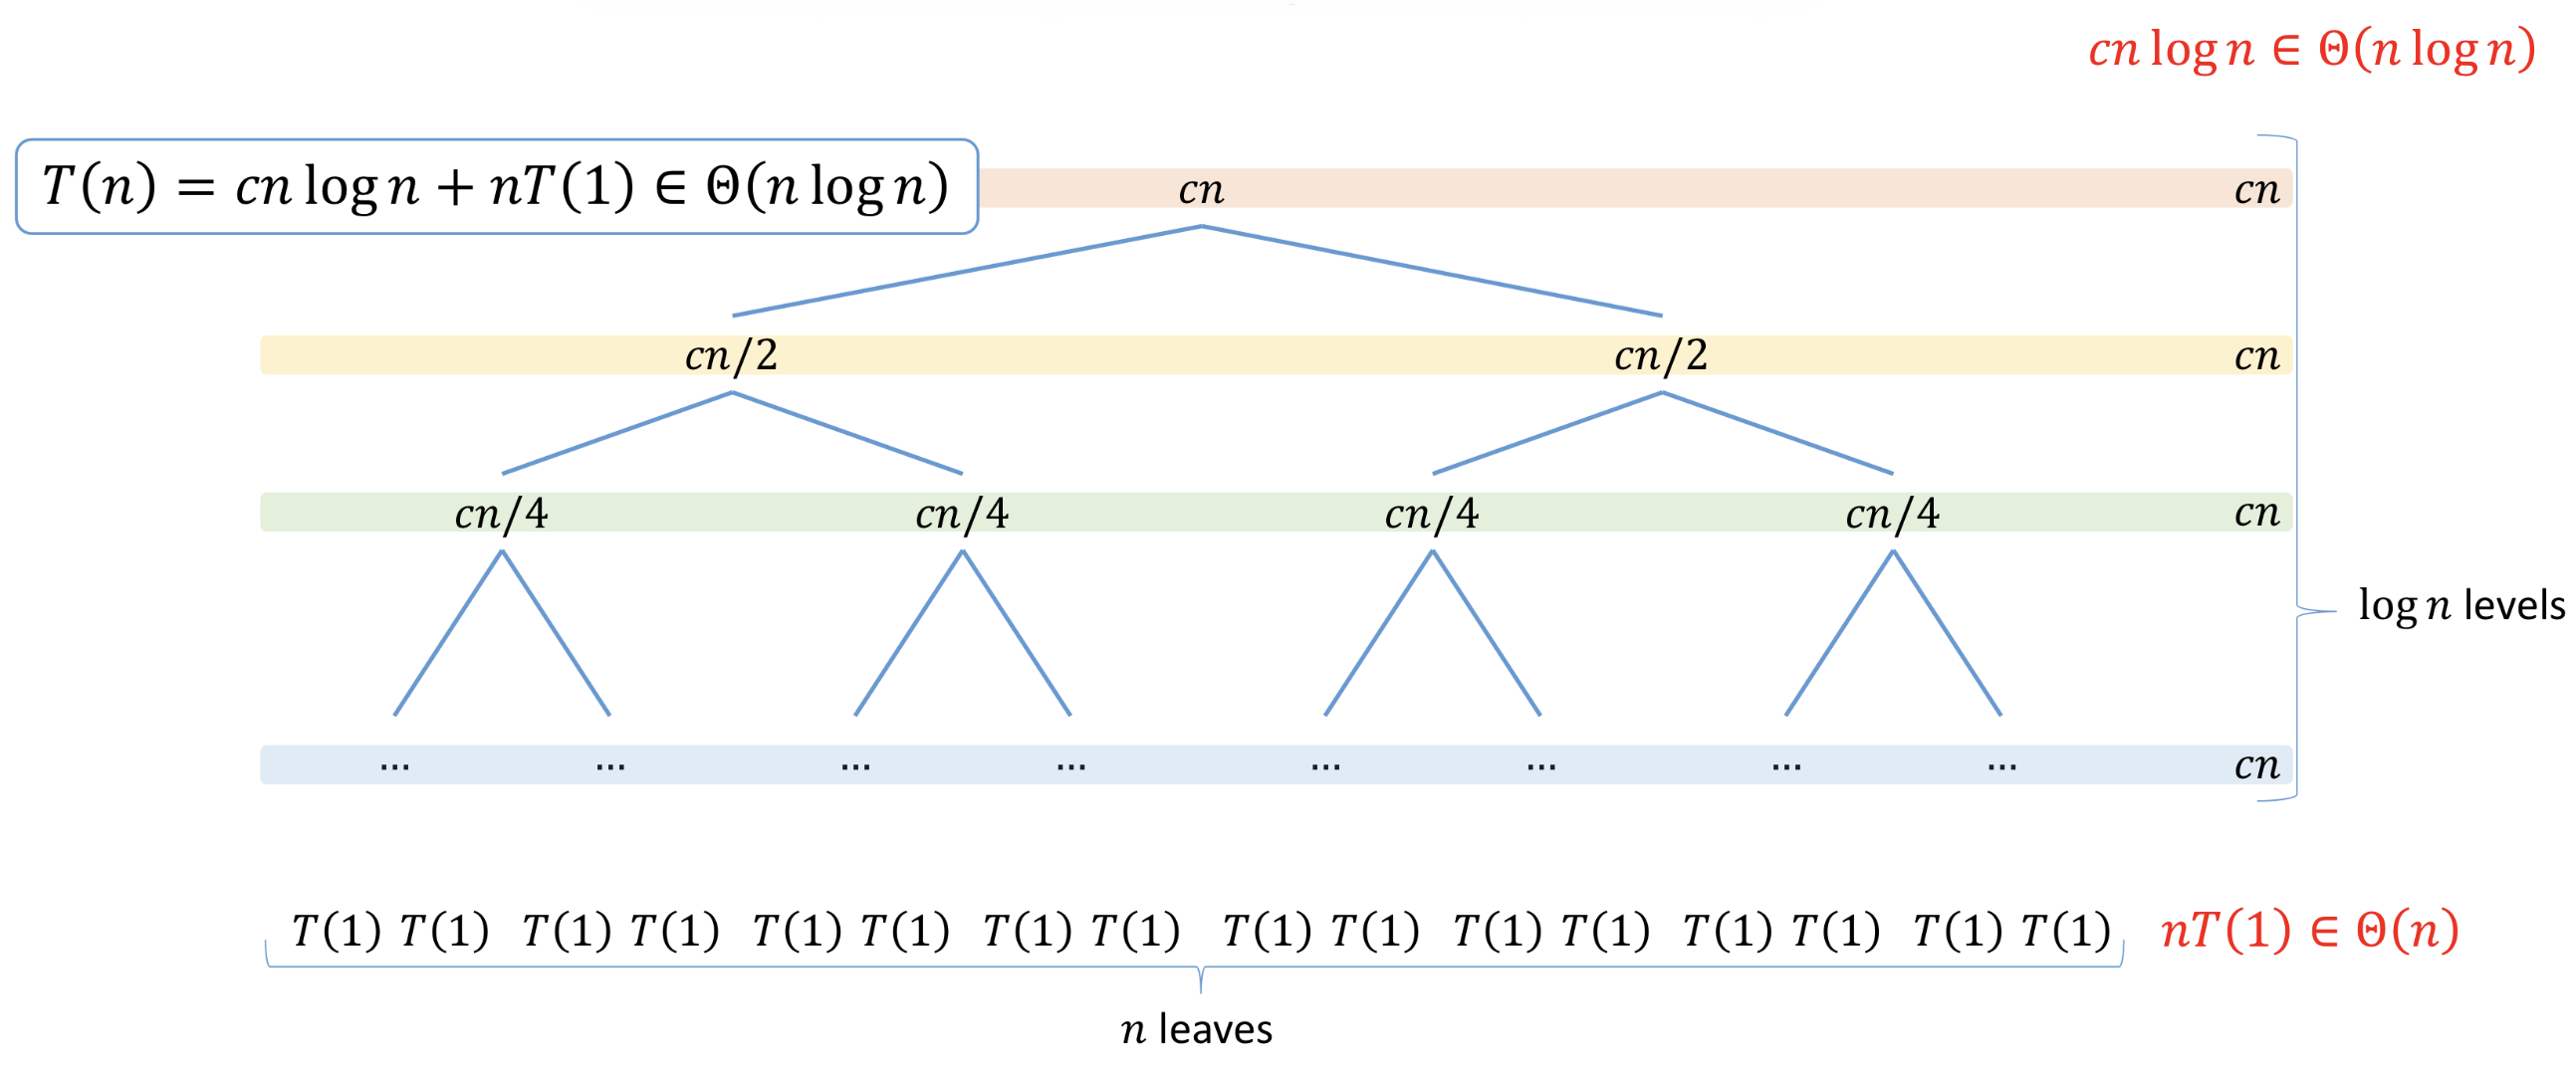
\includegraphics[width=0.55\linewidth]{recursion-tree.png}
  \caption{A recursion tree for $T(n) = aT(n/b) + f(n)$. Level $i$ contains $a^i$ nodes, each contributing $f(n/b^i)$; the tree has $\log_b n$ levels and $n^{\log_b a}$ leaves.}
  \label{fig:rec_tree}
\end{figure}

\begin{example}[Recursion tree for $T(n) = 2T(n/2) + cn$]
\label{ex:rec_tree_mergesort}
Consider $T(n) = 2T(n/2) + cn$ with $T(1) = \Theta(1)$, drawn as in \cref{fig:rec_tree}. The root contributes $cn$. Each of the two children contributes $cn/2$, so level $1$ totals $2 \cdot cn/2 = cn$. By induction, level $i$ totals $2^i \cdot c\,(n/2^i) = cn$. The tree has $\log_2 n$ levels and $n$ leaves, each of cost $T(1) = \Theta(1)$. Summing,
\[
  T(n) \;=\; \underbrace{cn \cdot \log_2 n}_{\text{splitting/combining work}} \;+\; \underbrace{n \cdot \Theta(1)}_{\text{base cases}}
  \;=\; \Theta(n \log n).
\]
The cost is uniform across levels; the log factor is exactly the height. This is the canonical case-2 picture.
\end{example}

\subsection{Master Theorem}

The master theorem is a \emph{look-up table} for divide-and-conquer recurrences. Given $T(n) = a T(n/b) + f(n)$ with $a \ge 1$ and $b > 1$, one computes the critical exponent $d = \log_b a$, compares $f(n)$ to $n^d$, and reads off the answer. The decision procedure is summarised in \cref{fig:mt_cases}; the case-3 branch additionally requires a \emph{regularity condition} on $f$.

\begin{figure}[h]
  \centering
  % Master Theorem case-decision tree.
% Inputs: T(n) = a T(n/b) + f(n), with a >= 1, b > 1.
\begin{tikzpicture}[
  every node/.style={font=\small\sffamily, align=center},
  decision/.style={draw, rounded corners=2pt, inner sep=4pt},
  leaf/.style={draw, dashed, rounded corners=2pt, inner sep=4pt},
  ->, >={Stealth[length=2mm]}
]
  \node[decision] (root) {Compare $f(n)$ to $n^{\log_b a}$};
  \node[decision, below left=1.0cm and 1.5cm of root]   (c1) {$f(n) = O(n^{\log_b a - \varepsilon})$\\ for some $\varepsilon > 0$?};
  \node[decision, below=1.0cm of root]                  (c2) {$f(n) = \Theta(n^{\log_b a})$?};
  \node[decision, below right=1.0cm and 1.5cm of root]  (c3) {$f(n) = \Omega(n^{\log_b a + \varepsilon})$\\ for some $\varepsilon > 0$,\\ and regularity holds?};
  \node[leaf, below=0.8cm of c1] (l1) {Case 1:\\ $T(n) = \Theta(n^{\log_b a})$};
  \node[leaf, below=0.8cm of c2] (l2) {Case 2:\\ $T(n) = \Theta(n^{\log_b a} \log n)$};
  \node[leaf, below=0.8cm of c3] (l3) {Case 3:\\ $T(n) = \Theta(f(n))$};
  \draw (root) -- (c1);
  \draw (root) -- (c2);
  \draw (root) -- (c3);
  \draw (c1) -- (l1) node[midway, right] {yes};
  \draw (c2) -- (l2) node[midway, right] {yes};
  \draw (c3) -- (l3) node[midway, right] {yes};
\end{tikzpicture}

  \caption{Master Theorem -- case selection. The critical exponent $d = \log_b a$ counts leaves of the recursion tree; $f(n)$ is the per-call splitting/combining cost.}
  \label{fig:mt_cases}
\end{figure}

\begin{theorem}[Master theorem]
\label{thm:master}
Let $T(n) = a\,T(n/b) + f(n)$ with constants $a \ge 1$, $b > 1$, and $f(n) \in \Omega(1)$. Set the critical exponent $d = \log_b a$. Then:
\begin{enumerate}[(1)]
  \item \emph{Leaves dominate.} If $f(n) = O(n^{d - \varepsilon})$ for some constant $\varepsilon > 0$, then $T(n) = \Theta(n^d)$.
  \item \emph{Comparable.} If $f(n) = \Theta(n^d \log^k n)$ for some constant $k \ge 0$, then $T(n) = \Theta(n^d \log^{k+1} n)$.
  \item \emph{Root dominates.} If $f(n) = \Omega(n^{d + \varepsilon})$ for some constant $\varepsilon > 0$, \emph{and} the \emph{regularity condition} $a\,f(n/b) \le c\,f(n)$ holds for some constant $c < 1$ and all sufficiently large $n$, then $T(n) = \Theta(f(n))$.
\end{enumerate}
\end{theorem}

\begin{proof}
\sketchproof Unroll the recurrence to a tree of height $\log_b n$, in which level $i$ contains $a^i$ nodes each of cost $f(n/b^i)$, with $a^{\log_b n} = n^d$ leaves of cost $T(1)$. The total cost is
\[
  T(n) \;=\; \underbrace{\sum_{i=0}^{\log_b n - 1} a^i\,f(n/b^i)}_{\text{splitting/combining}}
  \;+\; \underbrace{n^d \cdot T(1)}_{\text{base cases}}.
\]
The base-case total is $\Theta(n^d)$. The splitting/combining sum is the geometric series whose ratio between successive levels is $a / b^{e}$ where $e$ is the exponent of $f$.

\emph{Case 1.} If $f(n) = O(n^{d - \varepsilon})$, then $a^i f(n/b^i) \le c \cdot n^{d-\varepsilon} \cdot (a/b^{d-\varepsilon})^i = c\,n^{d-\varepsilon} \cdot b^{i\varepsilon}$ (using $b^d = a$). Summing the geometric series in $b^\varepsilon > 1$ over $\log_b n$ levels gives $O(n^{d-\varepsilon} \cdot b^{\varepsilon \log_b n}) = O(n^{d-\varepsilon} \cdot n^\varepsilon) = O(n^d)$. The leaf contribution $\Theta(n^d)$ dominates, so $T(n) = \Theta(n^d)$.

\emph{Case 2.} With $f(n) = \Theta(n^d \log^k n)$, level $i$ contributes $a^i \cdot \Theta((n/b^i)^d \log^k(n/b^i)) = \Theta(n^d \log^k(n/b^i))$, since $a^i (n/b^i)^d = n^d$. Summing over $i = 0, \dots, \log_b n - 1$ gives $\Theta(n^d) \cdot \sum_{i=0}^{\log_b n - 1} (\log n - i \log b)^k = \Theta(n^d \log^{k+1} n)$ (the standard sum $\sum_{j=1}^{m} j^k = \Theta(m^{k+1})$ for $k \ge 0$). The leaf cost $\Theta(n^d)$ is dominated by this, hence $T(n) = \Theta(n^d \log^{k+1} n)$. The familiar $k = 0$ subcase recovers $T(n) = \Theta(n^d \log n)$.

\emph{Case 3.} The regularity condition $af(n/b) \le c\,f(n)$ with $c < 1$ means the splitting cost shrinks geometrically as we descend the tree, so iteratively $a^i f(n/b^i) \le c^i f(n)$. The total splitting/combining cost is at most $f(n) \sum_{i \ge 0} c^i = f(n)/(1-c) = O(f(n))$, and at least $f(n)$ (the root alone). The leaf cost $n^d \cdot T(1)$ is $o(f(n))$ because $f(n) = \Omega(n^{d+\varepsilon})$. Hence $T(n) = \Theta(f(n))$.

\medskip
\noindent\textit{Remark.} Floors and ceilings can be ignored: for the recurrence $T(n) = a\,T(\lfloor n/b \rfloor) + f(n)$ the same conclusions hold, because the difference $\lfloor n/b \rfloor$ vs.\ $n/b$ contributes only a lower-order perturbation. The condition $f(n) = \Omega(n^{d+\varepsilon})$ in case 3 is in fact \emph{redundant} given the regularity condition (the regularity condition by itself implies a polynomial separation), but stating both is the standard convention.
\end{proof}

\begin{remark}[Hypotheses, gaps, and fallbacks]
\label{rem:master_gaps}
The form of \cref{thm:master} above requires $a \ge 1$, $b > 1$, and a non-negative driving function $f$. Recurrences like $T(n) = (1/2)\,T(n/2) + n$ ($a < 1$) and subtractive recurrences like $T(n) = T(n-1) + n$ or $T(n) = T(n-1) + T(1) + cn$ (the worst-case quicksort recurrence) are \emph{not} of the form $a\,T(n/b) + f(n)$ and must be solved by telescoping or a direct recursion-tree sum -- the worst-case quicksort recurrence, for instance, gives $\Theta(n^2)$, not $\Theta(n \log n)$.

Beyond hypothesis failures, even within the theorem's scope the standard statement does not cover every regime. The case-2 clause of \cref{thm:master} is restricted to $k \ge 0$. The \emph{extended master theorem} handles the remaining $\log^k$ exponents: for $f(n) = \Theta(n^d \log^k n)$ with $k > -1$ the conclusion $T(n) = \Theta(n^d \log^{k+1} n)$ still holds; with $k = -1$, $T(n) = \Theta(n^d \log\log n)$; with $k < -1$, $T(n) = \Theta(n^d)$. These are extensions beyond \cref{thm:master}. For exotic driving functions outside every $\log^k$-class -- for example $f(n) = 2^{\sqrt{\log n}}$ in $T(n) = T(n/2) + f(n)$ -- the recursion-tree method computes the actual sum directly. The Akra--Bazzi theorem generalises the master theorem to mixed-split recurrences such as $T(n) = T(n/3) + T(2n/3) + n$ and to a wider class of driving functions, at the cost of an integral evaluation in place of the case look-up.
\end{remark}

\begin{remark}[Case 3's regularity condition is non-negotiable]
\label{rem:master_regularity}
The polynomial-separation clause $f(n) \in \Omega(n^{d+\varepsilon})$ alone does not suffice for case 3. Even when polynomial separation holds, the regularity condition $a\,f(n/b) \le c\,f(n)$ for some $c < 1$ is a separate requirement that must be verified independently: it encodes the geometric decay of the per-level cost as one descends the recursion tree, and without it the proof of case 3 breaks down. Always verify regularity explicitly with a concrete $c < 1$, as illustrated by the verification step in \cref{ex:mt_case3}.
\end{remark}

\begin{example}[Master theorem case 1: $T(n) = 9T(n/3) + n$]
\label{ex:mt_case1}
Here $a = 9$, $b = 3$, so $d = \log_3 9 = 2$. The driving function is $f(n) = n = O(n^{2 - 1}) = O(n^{d - \varepsilon})$ for $\varepsilon = 1 > 0$. We are in case 1 of \cref{thm:master}, so $T(n) = \Theta(n^d) = \Theta(n^2)$. Intuitively the work is leaf-dominated: there are $9^{\log_3 n} = n^2$ leaves, each contributing $\Theta(1)$, which already accounts for $\Theta(n^2)$ work; the per-level $f(n)$ is too small to add anything beyond a constant factor.
\end{example}

\begin{example}[Master theorem case 2: $T(n) = 2T(n/2) + n$ (mergesort)]
\label{ex:mt_case2}
Here $a = 2$, $b = 2$, so $d = \log_2 2 = 1$. The driving function is $f(n) = n = \Theta(n^1 \log^0 n) = \Theta(n^d \log^k n)$ with $k = 0 \ge 0$. Case 2 of \cref{thm:master} gives $T(n) = \Theta(n^d \log^{k+1} n) = \Theta(n \log n)$. This reproduces the recursion-tree analysis of \cref{ex:rec_tree_mergesort}: every level of the tree contributes $cn$, there are $\log n$ levels, and the leaves contribute another $\Theta(n)$ subsumed by the level sum. Mergesort, the standard divide-and-conquer presentation of any $O(n)$-work merge step, the in-place mergesort, and Strassen's matrix multiplication all have case-2-style recurrences.
\end{example}

\begin{example}[Master theorem case 3: $T(n) = 3T(n/4) + n \log n$]
\label{ex:mt_case3}
Here $a = 3$, $b = 4$, so $d = \log_4 3 \approx 0.793$. The driving function is $f(n) = n \log n$. We check case 3.

\medskip
\noindent\textit{Polynomial separation.} For any $\varepsilon$ with $0 < \varepsilon < 1 - \log_4 3 \approx 0.207$, $f(n) = n \log n = \Omega(n^{1}) = \Omega(n^{d + \varepsilon})$, since $n \log n / n^{d+\varepsilon} = n^{1 - d - \varepsilon} \log n \to \infty$ as $n \to \infty$. So $f(n) \in \Omega(n^{d + \varepsilon})$.

\medskip
\noindent\textit{Regularity.} Need $a\,f(n/b) \le c\,f(n)$ for some $c < 1$. Compute
\[
  a\,f(n/b) \;=\; 3 \cdot (n/4) \log(n/4) \;=\; (3/4)\,n\,(\log n - 2) \;\le\; (3/4)\,n \log n \;=\; (3/4)\,f(n).
\]
So the regularity condition holds with $c = 3/4 < 1$. Both clauses of case 3 are satisfied; \cref{thm:master} concludes $T(n) = \Theta(f(n)) = \Theta(n \log n)$. The work is root-dominated: at the top level we already pay $n \log n$, and the sum across all $\log_4 n$ levels is bounded by $(1 + 3/4 + (3/4)^2 + \dots) \cdot f(n) = O(f(n))$.
\end{example}


% Chapter 4: Correctness.
\section{Correctness}
\label{sec:correctness}

An algorithm is \emph{correct} on a given input if, when executed, it halts and produces the specified output, and \emph{correct} (without qualification) if it is correct on every legal input. Correctness has two faces: \emph{partial correctness} (\emph{if} the algorithm halts, the output satisfies the post-condition) and \emph{termination}; together these constitute \emph{total correctness}. Iterative algorithms admit a uniform partial-correctness template -- the loop-invariant theorem -- with termination argued separately by exhibiting a non-negative integer variant. Recursive algorithms are handled by strong induction on input size.

\subsection{Definitions}

\begin{definition}[Loop invariant]
\label{def:loop_invariant}
\index{loop invariant}
A \emph{loop invariant} for a loop $L$ is a predicate $I$ on the program state such that $I$ holds at the start of every iteration of $L$ (equivalently, every time control reaches the loop guard). The invariant is the inductive hypothesis used to prove partial correctness of the loop: it must be (a) true on entry, (b) preserved by each pass of the loop body, and (c) strong enough that, combined with the negated guard, it implies the desired post-condition when the loop exits. Choosing the right invariant is the only creative step in a loop-invariant proof; everything else is mechanical.
\end{definition}

\begin{definition}[Partial correctness]
\label{def:partial_correctness}
\index{partial correctness}
An algorithm $\mathcal{A}$ is \emph{partially correct} with respect to a pre-condition $P$ and post-condition $Q$ if, for every input satisfying $P$, \emph{if} $\mathcal{A}$ halts on that input \emph{then} the output satisfies $Q$. Partial correctness says nothing about whether the algorithm halts; an algorithm that loops forever on every input is vacuously partially correct.
\end{definition}

\begin{definition}[Total correctness]
\label{def:total_correctness}
\index{total correctness}
An algorithm $\mathcal{A}$ is \emph{totally correct} with respect to $(P, Q)$ if, for every input satisfying $P$, $\mathcal{A}$ halts and the output satisfies $Q$. Equivalently, total correctness is partial correctness (\cref{def:partial_correctness}) plus termination. The two are typically established by separate arguments: the loop invariant or strong induction handles partial correctness, while a termination measure (\cref{def:termination_measure}) handles termination.
\end{definition}

\begin{definition}[Termination measure / variant]
\label{def:termination_measure}
\index{termination measure}
A \emph{termination measure} (or \emph{loop variant}) for a loop $L$ is a function $\mu$ from the program state into $\mathbb{N}$ (or, more generally, into a well-founded set such as $(\mathbb{N}, <)$) such that:
\begin{enumerate}[(i)]
  \item $\mu \ge 0$ at every point in the execution of $L$;
  \item $\mu$ \emph{strictly decreases} on every pass of the loop body, i.e.\ if $\mu_t$ is the value at the start of iteration $t$, then $\mu_{t+1} < \mu_t$.
\end{enumerate}
Since a strictly decreasing sequence of non-negative integers cannot be infinite, the existence of such a $\mu$ proves that $L$ executes only finitely many iterations. For recursive procedures the analogue is a measure on the input that strictly decreases on every recursive call; well-foundedness then forbids infinite recursion. Typical choices: $\mu = n - i$ for a \texttt{for} loop running from $i$ to $n$; $\mu = \mathrm{ub} - \mathrm{lb} + 1$ for binary search; $\mu = |V \setminus R|$ for Dijkstra's main loop.
\end{definition}

\begin{remark}[Well-founded, not merely decreasing]
The codomain of $\mu$ must be well-founded; strict decrease alone is not enough. A strictly decreasing sequence in $\mathbb{Q}$ or $\mathbb{R}$ can be infinite ($1, 1/2, 1/4, \dots$), so picking $\mathbb{N}$ (or any well-founded order) is essential. Conversely, ``the value of $i$ never repeats'' does not suffice -- $i$ must \emph{decrease} (or progress monotonically toward a fixed bound).
\end{remark}

\begin{definition}[Strong induction]
\label{def:strong_induction}
\index{strong induction}
\emph{Strong induction} (also \emph{course-of-values induction}) on $\mathbb{N}$: to prove that a predicate $P(n)$ holds for every $n \ge 0$, it suffices to prove
\[
  \forall n \in \mathbb{N},\ \bigl(\forall k < n,\ P(k)\bigr) \implies P(n).
\]
The base case $P(0)$ is the instance of this implication at $n = 0$, where the antecedent $\forall k < 0,\ P(k)$ is vacuous. Strong induction differs from ordinary induction only in the inductive hypothesis: instead of assuming $P(n-1)$ alone, we may assume $P(k)$ for \emph{all} $k < n$. The two principles are logically equivalent, but strong induction is the natural fit when a recursive procedure makes calls of varying smaller sizes (e.g.\ $\mathrm{Fib}(n)$ calls both $\mathrm{Fib}(n-1)$ and $\mathrm{Fib}(n-2)$).
\end{definition}

\begin{definition}[Structural induction]
\label{def:structural_induction}
\index{structural induction}
\emph{Structural induction} generalises strong induction from $\mathbb{N}$ to any \emph{inductively defined} (algebraic) structure: lists, trees, formulas, etc. To prove that a predicate $P$ holds for every element of such a structure, one proves $P$ for each base constructor (e.g.\ the empty list, a leaf), and proves $P$ for each recursive constructor under the assumption that $P$ holds for every immediate substructure (e.g.\ the tail of a list, the children of an internal node). Termination of recursion on the structure is automatic because the substructures are strictly smaller in the well-founded ordering induced by the constructors. In algorithm analysis, most correctness proofs reduce to strong induction (\cref{def:strong_induction}) on the integer input size; structural induction is the right tool whenever the input is naturally a tree or a recursive data type.
\end{definition}

\subsection{Loop invariants}

The loop-invariant pattern reduces partial correctness of an iterative algorithm to a three-line induction.

\begin{theorem}[Loop-invariant theorem]
\label{thm:loop_invariant_theorem}
Let $L$ be a loop with guard $G$ and let $I$ be a predicate on the program state. Suppose:
\begin{enumerate}[(i)]
  \item \emph{(Initialisation)} $I$ holds at the start of the first iteration;
  \item \emph{(Maintenance)} for every iteration $t$, if $I$ and $G$ hold at the start of $t$, then $I$ holds at the start of iteration $t+1$ (equivalently, at the end of iteration $t$);
  \item \emph{(Termination)} the loop performs only finitely many iterations.
\end{enumerate}
Then, when $L$ exits, the conjunction $I \wedge \neg G$ holds. Consequently, if $I \wedge \neg G$ entails the desired post-condition, the loop is partially correct, and -- given (iii) -- totally correct.
\end{theorem}

\begin{proof}
Let $I_t$ denote ``$I$ holds at the start of iteration $t$''. We prove by induction on $t$ that $I_t$ holds for every $t = 1, 2, \dots, T$, where $T$ is the total number of iterations (finite by (iii)). The base case $t = 1$ is exactly (i). For the inductive step, suppose $I_t$ holds. Either iteration $t$ is the last one (the guard becomes false, and $I_t$ remains true at exit, so $I_{T+1} := I$-at-exit holds), or iteration $t$ executes the body and control returns to the guard; by (ii) this implies $I_{t+1}$. By induction, $I$ holds at the moment the loop exits. At that moment the guard is false (else the loop would have continued), so $I \wedge \neg G$ holds, as claimed. The post-condition then follows by the assumed entailment $I \wedge \neg G \models Q$.
\end{proof}

\begin{remark}[Three obligations $\leftrightarrow$ induction]
The structure of \cref{thm:loop_invariant_theorem} is exactly mathematical induction on iteration count: initialisation is the base case, maintenance is the inductive step, and the ``termination'' clause names the conclusion drawn at exit (not to be confused with proving the loop terminates -- that is a separate obligation handled by a variant, \cref{def:termination_measure}). Some authors fold the post-condition entailment into a fourth bullet called ``termination''; we bundle ``invariant survives plus guard fails $\Rightarrow$ correct output'' into a single observation.
\end{remark}

\begin{remark}[Common loop-invariant pitfalls]
Three slips recur. First, partial correctness is not total correctness: the loop-invariant theorem gives only conditional correctness, so a separate termination argument (a variant in $\mathbb{N}$ that strictly decreases, \cref{def:termination_measure}) is still owed. Second, the invariant must survive \emph{exit}: it is $I \wedge \neg G$ at the moment the guard fails that must imply the post-condition, so a candidate $I$ too weak to do so when conjoined with $\neg G$ is not yet finished. Third, the boundary case of zero iterations matters: if the body is never executed (e.g.\ $n = 0$ in selection sort, or $\mathrm{lb} > \mathrm{ub}$ in binary search), initialisation and the negated guard alone must already entail the post-condition, typically by appealing to vacuous truth (an empty prefix is sorted, an empty range contains no element) -- but this should be stated explicitly.
\end{remark}

\begin{example}[Selection sort -- finding the right invariant]
\label{ex:insertion_sort_correctness}
We prove the partial correctness of \textsc{SelectionSort}, the sorting algorithm given in \cref{alg:selection_sort}.

\begin{algorithm}
\caption{\textsc{SelectionSort}$(A[1..n])$.}
\label{alg:selection_sort}
\begin{algorithmic}[1]
  \For{$j = 1$ \textbf{to} $n - 1$}
    \State Select $s \in \{j, j+1, \dots, n\}$ such that $A[s]$ is a smallest entry in $A[j..n]$.
    \State Swap $A[j]$ and $A[s]$.
  \EndFor
\end{algorithmic}
\end{algorithm}

\noindent\textbf{Choice of invariant.} Three candidate invariants ``at the start of iteration $j$'' suggest themselves:
\begin{enumerate}[(a)]
  \item ``$A$ is sorted.'' \emph{Fails initialisation:} a generic input is not sorted at the start of $j = 1$.
  \item ``$A[1..j-1]$ is sorted.'' Initialisation and termination check out (at exit $j = n$, so $A[1..n-1]$ is sorted, and one more element being out of place would break the post-condition only if $A[n]$ were smaller than $A[n-1]$). \emph{Fails maintenance:} nothing forces $A[j-1] \le A[j]$, since the prefix sorted-ness of $A[1..j-1]$ does not constrain the relationship between the prefix and the suffix.
  \item ``$x \le y$ for all $x \in A[1..j-1]$ and $y \in A[j..n]$.'' \emph{Fails termination:} at exit, this only says the largest of the first $n-1$ entries is $\le A[n]$, which does not imply that the prefix itself is sorted.
\end{enumerate}
The fix is to conjoin (b) and (c). The correct invariant $I_j$ is:
\[
  \text{$A[1..j-1]$ is sorted}\quad \wedge \quad x \le y\ \text{for all } x \in A[1..j-1],\ y \in A[j..n].
\]

\medskip
\noindent\textit{Initialisation.} At $j = 1$, the prefix $A[1..0]$ is empty, so both conjuncts hold vacuously.

\medskip
\noindent\textit{Maintenance.} Suppose $I_j$ holds at the start of iteration $j$. Iteration $j$ picks $s \in \{j, \dots, n\}$ with $A[s] = \min A[j..n]$ and swaps $A[j]$ and $A[s]$. After the swap:
\begin{itemize}
  \item $A[1..j-1]$ is unchanged and remains sorted.
  \item The new $A[j]$ equals the old $A[s] = \min A[j..n]$, which by the second conjunct of $I_j$ is $\ge$ every $x \in A[1..j-1]$ (since each such $x$ was $\le$ every entry in $A[j..n]$). Hence $A[j-1] \le A[j]$, so $A[1..j]$ is sorted.
  \item The new $A[j]$ is also $\le$ every entry remaining in $A[j+1..n]$ (it was the minimum of $A[j..n]$). Combined with the second conjunct of $I_j$, every entry of $A[1..j]$ is $\le$ every entry of $A[j+1..n]$.
\end{itemize}
Both conjuncts of $I_{j+1}$ hold.

\medskip
\noindent\textit{Termination (post-condition).} The loop exits with $j = n$, at which point $I_n$ asserts that $A[1..n-1]$ is sorted and every entry of $A[1..n-1]$ is $\le A[n]$. Together this means $A[1..n]$ is sorted, which is the post-condition. (Termination of the loop itself is immediate: the \texttt{for} loop runs $n - 1$ times.)

\medskip
\noindent\textit{Why each candidate failed.} The lesson is that an invariant must be \emph{strong enough} to imply the post-condition at exit and \emph{weak enough} to be true at entry; (b) was too weak at the right (termination), while (a) was too strong at the left (initialisation). Conjoining (b) and (c) is the standard fix: a sorted prefix together with ``every prefix entry $\le$ every suffix entry'' is exactly the invariant that survives both endpoints. The methodological point generalises: pick the invariant \emph{before} writing the proof. Reverse-engineering one from the maintenance step is a common error. The candidate-checking exercise above -- write several candidates, mark which of (init / maint / term) each one satisfies, and conjoin until all three boxes are ticked -- is the right discipline.
\end{example}

\subsection{Termination}

Partial correctness is independent of termination, and termination is usually proved separately by exhibiting a variant.

\begin{example}[Binary search -- termination via a strictly decreasing variant]
\label{ex:binary_search_termination}
Consider \textsc{BinarySearch}$(A, \mathrm{lb}, \mathrm{ub}, x)$ in \cref{alg:binary_search}, which decides whether $x$ occurs in the sorted slice $A[\mathrm{lb}..\mathrm{ub}]$.

\begin{algorithm}
\caption{\textsc{BinarySearch}$(A, \mathrm{lb}, \mathrm{ub}, x)$.}
\label{alg:binary_search}
\begin{algorithmic}[1]
  \If{$\mathrm{lb} > \mathrm{ub}$} \Return \textbf{NO} \EndIf
  \State $\mathrm{mid} \gets \lfloor (\mathrm{lb} + \mathrm{ub})/2 \rfloor$.
  \If{$x = A[\mathrm{mid}]$} \Return \textbf{YES}
  \ElsIf{$x > A[\mathrm{mid}]$} \Return \textsc{BinarySearch}$(A, \mathrm{mid}+1, \mathrm{ub}, x)$
  \ElsIf{$x < A[\mathrm{mid}]$} \Return \textsc{BinarySearch}$(A, \mathrm{lb}, \mathrm{mid}-1, x)$
  \EndIf
\end{algorithmic}
\end{algorithm}

\noindent\textbf{Termination measure.} Let $n = \mathrm{ub} - \mathrm{lb} + 1$ be the size of the searched slice. Set $\mu = \max(n, 0)$; then $\mu \in \mathbb{N}$.

\medskip
\noindent\textit{$\mu$ strictly decreases at every recursive call.} Let $m = \lfloor (\mathrm{lb} + \mathrm{ub})/2 \rfloor$, so $\mathrm{lb} \le m \le \mathrm{ub}$ when the call is made (the early return at $\mathrm{lb} > \mathrm{ub}$ ensures $n \ge 1$ in this branch). The two recursive calls have new slice sizes
\[
  n_{\text{right}} = \mathrm{ub} - (m + 1) + 1 = \mathrm{ub} - m, \qquad
  n_{\text{left}}  = (m - 1) - \mathrm{lb} + 1 = m - \mathrm{lb}.
\]
Both are $\le \lfloor n/2 \rfloor \le n - 1 < n$ (when $n \ge 1$), so $\mu$ strictly decreases.

\medskip
\noindent\textit{$\mu \ge 0$.} Immediate from the definition.

\medskip
\noindent\textit{Conclusion.} A strictly decreasing sequence in $\mathbb{N}$ cannot be infinite, so the recursion bottoms out after at most $\mu_0$ levels, where $\mu_0$ is the initial value. In fact $\mu$ at least halves each level, so the recursion depth is $O(\log n)$, matching the well-known $O(\log n)$ time bound. The same variant $\mathrm{ub} - \mathrm{lb} + 1$ also works for the half-open-interval variant of binary search; the choice of $+1$ vs $-1$ affects only the off-by-one shift in the base case.
\end{example}

\subsection{Induction for recursive algorithms}

For a recursive procedure $\mathcal{A}$, correctness on every input reduces to two obligations: (a) the no-recursion (base) branches are correct, and (b) for every recursive branch, \emph{if} all recursive calls return correct answers, then so does the surrounding code. The combination is precisely strong induction (\cref{def:strong_induction}) on input size.

\begin{theorem}[Strong induction principle]
\label{thm:strong_induction}
Let $P(n)$ be a predicate on $\mathbb{N}$. If
\[
  \forall n \in \mathbb{N},\ \bigl(\forall k < n,\ P(k)\bigr) \implies P(n),
\]
then $P(n)$ holds for every $n \in \mathbb{N}$.
\end{theorem}

\begin{proof}
Define $Q(n) := \forall k \le n,\ P(k)$. We show $Q(n)$ for all $n$ by ordinary induction. \emph{Base} $n = 0$: the hypothesis at $n = 0$ has the vacuous antecedent $\forall k < 0,\ P(k)$, so it directly yields $P(0)$, hence $Q(0)$. \emph{Step:} suppose $Q(n)$, i.e.\ $P(k)$ for all $k \le n$; equivalently $P(k)$ for all $k < n+1$. The hypothesis at $n + 1$ then gives $P(n+1)$, so $Q(n+1)$ holds. By ordinary induction $Q(n)$ holds for every $n$, hence so does $P(n)$.

The same argument works for any well-founded relation in place of $<$ on $\mathbb{N}$, which is what justifies structural induction (\cref{def:structural_induction}) on inductively defined data types.
\end{proof}

\begin{remark}[When to reach for strong induction, and how many base cases]
If the recursive call is on a single argument with size exactly $n - 1$ (e.g.\ a tail-recursive linear scan), ordinary induction suffices. Strong induction is the right tool when the call is on a smaller-by-an-arbitrary-amount argument (binary search's $\lfloor n/2 \rfloor$) or when there are multiple recursive calls (Fibonacci, merge sort). A recursion that refers to both $f(n-1)$ and $f(n-2)$ also requires base cases at \emph{both} $n = 0$ and $n = 1$; otherwise the first recursive step appeals to $f(-1)$.
\end{remark}

\begin{example}[Recursive Fibonacci -- correctness by strong induction]
\label{ex:recursive_correctness}
Let $\mathrm{Fib}(n)$ be defined by $\mathrm{Fib}(0) = 0$, $\mathrm{Fib}(1) = 1$, and $\mathrm{Fib}(n) = \mathrm{Fib}(n-1) + \mathrm{Fib}(n-2)$ for $n \ge 2$. Consider the recursive algorithm
\[
  \textsc{Fib}(n) := \begin{cases} n & \text{if } n \le 1, \\ \textsc{Fib}(n-1) + \textsc{Fib}(n-2) & \text{otherwise.} \end{cases}
\]
We show that $\textsc{Fib}(n) = \mathrm{Fib}(n)$ for all $n \ge 0$ by strong induction (\cref{thm:strong_induction}) on $n$.

\medskip
\noindent\textit{Base cases.} For $n = 0$: $\textsc{Fib}(0) = 0 = \mathrm{Fib}(0)$. For $n = 1$: $\textsc{Fib}(1) = 1 = \mathrm{Fib}(1)$. Both are the $n \le 1$ branch and involve no recursion. Two base cases are needed because the recursive branch refers to $\textsc{Fib}(n-2)$ and $\textsc{Fib}(n-1)$ simultaneously.

\medskip
\noindent\textit{Inductive step.} Fix $n \ge 2$ and assume $\textsc{Fib}(k) = \mathrm{Fib}(k)$ for every $k$ with $0 \le k < n$. Since $n \ge 2$ the algorithm executes the recursive branch:
\[
  \textsc{Fib}(n) = \textsc{Fib}(n-1) + \textsc{Fib}(n-2)
  \stackrel{\text{IH}}{=} \mathrm{Fib}(n-1) + \mathrm{Fib}(n-2)
  = \mathrm{Fib}(n),
\]
where the second equality uses the inductive hypothesis at the two strictly smaller indices $n-1$ and $n-2$ (both $\ge 0$ because $n \ge 2$), and the third is the recurrence defining $\mathrm{Fib}$. By \cref{thm:strong_induction}, $\textsc{Fib}(n) = \mathrm{Fib}(n)$ for every $n \ge 0$.

\medskip
\noindent\textit{Termination.} Each recursive call strictly decreases the input ($n \mapsto n-1$ and $n \mapsto n-2$, both non-negative once $n \ge 2$), and the base branch returns at $n \le 1$. The variant $\mu = n$ is non-negative and strictly decreases on every recursive call, so by \cref{def:termination_measure} the recursion terminates. Total correctness follows.

\medskip
\noindent\textit{Why strong (not ordinary) induction.} The recursive branch invokes the algorithm at \emph{two} smaller arguments, $n-1$ and $n-2$. The inductive hypothesis must cover both, which is exactly the strength advantage of strong induction over $P(n-1) \Rightarrow P(n)$. The same pattern applies to merge sort (recursion on the two halves of size $\lfloor n/2 \rfloor$ and $\lceil n/2 \rceil$, both $< n$ for $n \ge 2$), to recursive binary search (induction on slice size $n = \mathrm{ub} - \mathrm{lb} + 1$, base case $n \le 0$ returning \textbf{NO}, inductive step splitting on $x$ vs $A[\mathrm{mid}]$ and invoking strong induction on a strictly smaller slice), and to fast exponentiation $\mathrm{power}(x, n) = \mathrm{power}(x, \lfloor n/2 \rfloor)^2 \cdot x^{n \bmod 2}$.
\end{example}



% --- Part II: Algorithm Design Paradigms ---
\part{Algorithm Design Paradigms}
% Chapter 5: Divide and Conquer.
\section{Divide and Conquer}
\label{sec:dnc}

Divide-and-conquer (D\&C) refines the brute-force / iterative approach by reducing an instance of size $n$ to several instances of the \emph{same problem} on strictly smaller inputs, recursing, and stitching the sub-answers back together. Running times then satisfy a recurrence of the canonical shape $T(n) = a T(n/b) + f(n)$ solved by the Master Theorem (\cref{thm:master}), and correctness follows by strong induction on $n$. The asymptotic cost is determined by a competition between the number of subproblems $a$ and the combine cost $f(n)$, a principle exploited by Strassen's algorithm and many others.

\subsection{Definitions}

\begin{definition}[Divide-and-conquer paradigm]
\label{def:dnc_paradigm}
\index{divide and conquer}
A \emph{divide-and-conquer} algorithm for a problem with input size $n$ proceeds in three steps:
\begin{enumerate}[(1)]
  \item \textbf{Divide.} Split the instance into $a \ge 1$ subinstances, each of size at most $n/b$ for some constant $b > 1$ (so subinstances are \emph{strictly smaller}).
  \item \textbf{Conquer.} Solve each subinstance recursively. When $n$ falls below a constant threshold the recursion is terminated by a direct base-case computation in $\Theta(1)$ time.
  \item \textbf{Combine.} Stitch the $a$ subinstance answers into an answer for the original instance.
\end{enumerate}
Writing $f(n)$ for the time spent on divide+combine on an instance of size $n$, the worst-case running time satisfies the canonical recurrence
\[
  T(n) \;=\;
  \begin{cases}
    \Theta(1) & \text{if } n \le n_0, \\
    a\,T(n/b) + f(n) & \text{if } n > n_0,
  \end{cases}
\]
for the constant base-case threshold $n_0$. The recursion-tree shape is determined by $(a, b)$ and the leaf-vs-root cost balance is determined by $f(n)$ versus $n^{\log_b a}$ (\cref{thm:master}).
\end{definition}

\begin{remark}[Why $b > 1$ strictly]
The strict inequality $b > 1$ is what makes D\&C terminate: each call is on an input strictly smaller than its parent, so after $\log_b n$ levels the recursion bottoms out. A recurrence such as $T(n) = 2T(n/1) + n$ or $T(n) = T(n) + 1$ does not describe a D\&C algorithm and does not terminate; this is the same reason recursive correctness proofs require the induction to be on a well-founded measure. When setting up the recurrence, always verify $n/b < n$ for the chosen $b$.
\end{remark}

\begin{remark}[State the combine cost explicitly]
A common slip is to write $T(n) = a T(n/b)$ with no $f(n)$ term, which silently asserts that the divide and combine steps cost $O(1)$. They rarely do: for naive matrix multiplication the combine is $\Theta(n^2)$, for Strassen's algorithm it is also $\Theta(n^2)$ (eighteen block additions), and for the closest-pair-of-points problem it is $\Theta(n)$ via the strip argument. Always identify $f(n)$ before invoking the Master Theorem.
\end{remark}

\subsection{Key results}

\begin{theorem}[Correctness template for D\&C]
\label{thm:dnc_correctness}
Let $\mathcal{A}$ be a D\&C algorithm in the form of \cref{def:dnc_paradigm}, with base case correct by direct inspection and a combine step which, given correct answers for the $a$ subinstances, produces a correct answer for the parent instance. Then $\mathcal{A}$ is correct on every input.
\end{theorem}

\begin{proof}
Strong induction on $n$, the size of the input.

\smallskip
\noindent\emph{Base case.} For $n \le n_0$, the algorithm returns the value computed by the direct base-case routine, which is correct by hypothesis.

\smallskip
\noindent\emph{Inductive step.} Fix $n > n_0$ and assume (strong inductive hypothesis) that $\mathcal{A}$ is correct on every input of size $< n$. On an input of size $n$, $\mathcal{A}$ first divides into $a$ subinstances each of size at most $n/b < n$. By the inductive hypothesis, the recursive calls return correct answers for these $a$ subinstances. By the assumption on the combine step, the algorithm then produces a correct answer for the parent. Hence $\mathcal{A}$ is correct on the input of size $n$.

By strong induction, $\mathcal{A}$ is correct on every input.
\end{proof}

\begin{remark}[Match the base case to the algorithm]
The strong-induction proof above only goes through if the base case in the proof matches what the algorithm actually does. If the recursion bottoms out at threshold $n_0 > 1$ but the analysis writes $T(1) = T(0) = \Theta(1)$ to argue termination, the recurrence is still numerically correct but the inductive step has no anchor at $n = n_0$. State the base case at the size the algorithm actually terminates at.
\end{remark}

\begin{proposition}[Worst-case time of a D\&C algorithm]
\label{prop:dnc_complexity}
Let $\mathcal{A}$ be a D\&C algorithm whose running time satisfies the canonical recurrence $T(n) = a T(n/b) + f(n)$ with $a \ge 1$, $b > 1$, $f$ eventually positive. Let $c^* = \log_b a$. Then by the Master Theorem (\cref{thm:master}):
\begin{itemize}
  \item if $f(n) \in O(n^{c^* - \varepsilon})$ for some $\varepsilon > 0$, then $T(n) \in \Theta(n^{c^*})$ \emph{(leaves dominate)};
  \item if $f(n) \in \Theta(n^{c^*})$, then $T(n) \in \Theta(n^{c^*} \log n)$ \emph{(balanced)};
  \item if $f(n) \in \Omega(n^{c^* + \varepsilon})$ for some $\varepsilon > 0$ \emph{and} the regularity condition $a f(n/b) \le k f(n)$ holds for some $k < 1$ and all large $n$, then $T(n) \in \Theta(f(n))$ \emph{(root dominates)}.
\end{itemize}
\end{proposition}

\begin{proof}
\sketchproof This is exactly the Master Theorem (\cref{thm:master}), which is proved in \cref{sec:recurrences} by summing the per-level work in the recursion tree. Each of the $\log_b n$ levels has $a^k$ nodes at depth $k$, each doing work $f(n/b^k)$, so the total work is
\[
  T(n) \;=\; \sum_{k=0}^{\log_b n - 1} a^k f(n/b^k) \;+\; \Theta(a^{\log_b n}).
\]
The leaf term equals $\Theta(n^{\log_b a}) = \Theta(n^{c^*})$. Whether the geometric-like sum on the left is dominated by its first term, last term, or grows uniformly across levels, is exactly the case split on $f(n)$ versus $n^{c^*}$.
\end{proof}

\begin{remark}[The two levers of D\&C optimisation]
\Cref{prop:dnc_complexity} makes the two design levers explicit. To improve a D\&C algorithm one can either (i) reduce $a$ (fewer subproblems) which decreases $c^* = \log_b a$ and so shrinks the leaf term, or (ii) reduce $f(n)$ which only helps if $f(n)$ already dominates (Case 3) or matches (Case 2) the leaf term. In Case 1 the leaves already swamp the combine, so making the combine cheaper does not change the asymptotic cost. The recurrence $T(n) = 8T(n/2) + n^3$ illustrates this: original is $\Theta(n^3 \log n)$ (Case 2); dropping $f$ from $n^3$ to $n^2$ gives $\Theta(n^3)$ via Case 1 (where $f$ no longer matters), and dropping $a$ from $8$ to $7$ also gives $\Theta(n^3)$ but via Case 3, where regularity must be checked.
\end{remark}

\begin{remark}[Regularity and the divide step]
Case 3 of \cref{thm:master} requires the regularity condition $a f(n/b) \le k f(n)$ for some constant $k < 1$ and all large $n$. For polynomial $f$ this is automatic; for $f$ involving logarithms or other slowly-varying factors it must be verified, otherwise the Akra--Bazzi method (\cref{sec:recurrences}) is needed. A separate trap is the cost of the divide step itself: for closest-pair and similar geometric problems, sorting points by $x$-coordinate inside every recursive call would push the recurrence to $T(n) = 2T(n/2) + n \log n$, giving $\Theta(n \log^2 n)$ instead of the optimal $\Theta(n \log n)$. The standard fix --- pre-sort once, then pass sorted lists down through the recursion --- is itself a D\&C-design pattern.
\end{remark}

\subsection{Worked examples}

\begin{example}[Fast exponentiation by repeated squaring]
\label{ex:fast_exp}
\textbf{Problem.} Given a positive integer $a$ and a non-negative integer $n$, compute $a^n$ (in modular arithmetic, so each multiplication is $\Theta(1)$ in the word RAM model).

\medskip
\noindent\textbf{Naive approach.} The recurrence $a^n = a^{n-1} \cdot a$ gives $T(n) = T(n-1) + \Theta(1)$, hence $T(n) \in \Theta(n)$. This is iteration, not D\&C: the subinstance is of size $n - 1$, not $n / b$.

\medskip
\noindent\textbf{D\&C approach.} Use the identity
\[
  a^n \;=\;
  \begin{cases}
    \bigl(a^{\lfloor n/2 \rfloor}\bigr)^{\!2} & \text{if } n \text{ is even}, \\
    \bigl(a^{\lfloor n/2 \rfloor}\bigr)^{\!2} \cdot a & \text{if } n \text{ is odd}.
  \end{cases}
\]
\textit{Divide:} reduce computing $a^n$ to a single subproblem of computing $a^{\lfloor n/2 \rfloor}$. \textit{Conquer:} recurse to obtain $x = a^{\lfloor n/2 \rfloor}$. \textit{Combine:} return $x \cdot x$ (or $x \cdot x \cdot a$ if $n$ is odd), $\Theta(1)$ work.

\medskip
\noindent\textbf{Pseudocode.}
\begin{algorithmic}
\Function{FastExp}{$a, n$}
  \If{$n = 0$} \Return $1$ \EndIf
  \State $x \gets$ \Call{FastExp}{$a, \lfloor n/2 \rfloor$}
  \If{$n$ is even} \Return $x \cdot x$
  \Else{} \Return $x \cdot x \cdot a$
  \EndIf
\EndFunction
\end{algorithmic}

\medskip
\noindent\textbf{Correctness.} By \cref{thm:dnc_correctness}: base case $n = 0$ returns $1 = a^0$. For $n > 0$, by strong induction the recursive call returns $x = a^{\lfloor n/2 \rfloor}$ correctly; the combine step then returns $x^2 = a^{2\lfloor n/2 \rfloor}$ which equals $a^n$ when $n$ is even and $a^{n-1}$ when $n$ is odd, in which case multiplying by $a$ gives $a^n$.

\medskip
\noindent\textbf{Time.} The recurrence is $T(n) = T(n/2) + \Theta(1)$, so $a = 1$, $b = 2$, $f(n) = \Theta(1)$, $c^* = \log_2 1 = 0$. Since $f(n) = \Theta(n^0) = \Theta(n^{c^*})$, Case 2 of \cref{prop:dnc_complexity} (\cref{thm:master}) gives
\[
  T(n) \;\in\; \Theta(n^0 \log n) \;=\; \Theta(\log n).
\]
This is an exponential improvement over the iterative $\Theta(n)$. The same idea, applied to a $2 \times 2$ companion matrix $M = \begin{psmallmatrix} 1 & 1 \\ 1 & 0 \end{psmallmatrix}$, gives an $O(\log n)$-time algorithm for the $n$-th Fibonacci number via $M^n = \begin{psmallmatrix} F_{n+1} & F_n \\ F_n & F_{n-1} \end{psmallmatrix}$.
\end{example}

\begin{example}[Strassen's matrix multiplication, $\Theta(n^{\log_2 7})$]
\label{ex:strassen}
\textbf{Problem.} Given two $n \times n$ matrices $A$ and $B$ (assume $n$ is a power of $2$ for cleanliness), compute $C = A \cdot B$.

\medskip
\noindent\textbf{Naive D\&C.} Block-partition each matrix into four $(n/2) \times (n/2)$ blocks:
\[
  A = \begin{pmatrix} a & b \\ c & d \end{pmatrix},\quad
  B = \begin{pmatrix} e & f \\ g & h \end{pmatrix},\quad
  C = \begin{pmatrix} r & s \\ t & u \end{pmatrix},
\]
where the entries $a, \dots, h, r, \dots, u$ are themselves $(n/2) \times (n/2)$ matrices and
\[
  r = ae + bg,\quad s = af + bh,\quad t = ce + dg,\quad u = cf + dh.
\]
\textit{Divide+combine cost:} 4 block-additions of $(n/2)$-square matrices, $\Theta(n^2)$ total. \textit{Conquer:} 8 block-multiplications of $(n/2)$-square matrices. The recurrence is $T(n) = 8 T(n/2) + \Theta(n^2)$, with $c^* = \log_2 8 = 3$ and $f(n) = \Theta(n^2) = O(n^{3-1})$ in Case 1, hence $T(n) \in \Theta(n^3)$. No improvement over the standard triple-loop algorithm.

\medskip
\noindent\textbf{Strassen's trick.} Following \cref{prop:dnc_complexity}, the leaves dominate ($f(n) \ll n^{c^*}$), so the only way to improve the asymptotic is to reduce $a = 8$. Strassen (1969) computes $C = AB$ using only \emph{seven} block-multiplications, at the cost of $18$ block-additions/subtractions:
\[
  \begin{array}{ll}
    P_1 = a (f - h),         & P_5 = (a + d)(e + h), \\
    P_2 = (a + b) h,         & P_6 = (b - d)(g + h), \\
    P_3 = (c + d) e,         & P_7 = (a - c)(e + f), \\
    P_4 = d (g - e),         &
  \end{array}
\]
and then
\[
  r = P_5 + P_4 - P_2 + P_6,\quad s = P_1 + P_2,\quad t = P_3 + P_4,\quad u = P_5 + P_1 - P_3 - P_7.
\]

\medskip
\noindent\textbf{Correctness.} A direct expansion verifies each formula; for instance,
\begin{align*}
  P_5 + P_4 - P_2 + P_6
  &= (a+d)(e+h) + d(g-e) - (a+b)h + (b-d)(g+h) \\
  &= ae + ah + de + dh + dg - de - ah - bh + bg + bh - dg - dh \\
  &= ae + bg \;=\; r,
\end{align*}
and similarly for $s, t, u$. Note: the $P_i$ are products of $(n/2)$-square matrices, so they do \emph{not} commute with each other, but each $P_i$ is a single matrix product, so the algebraic identities only require associativity and distributivity, both of which matrix arithmetic satisfies. Combined with \cref{thm:dnc_correctness}, the algorithm is correct.

\medskip
\noindent\textbf{Time.} Now $a = 7$, $b = 2$, $f(n) = \Theta(n^2)$ (the 18 block-additions). So $c^* = \log_2 7 \approx 2.807$ and $f(n) = \Theta(n^2) = O(n^{c^* - \varepsilon})$ for any $\varepsilon < c^* - 2$. Case 1 of \cref{prop:dnc_complexity} gives
\[
  T(n) \;\in\; \Theta\bigl(n^{\log_2 7}\bigr) \;=\; \Theta(n^{2.807\dots}).
\]

\medskip
\noindent\textbf{Remark.} Strassen's algorithm is the proof-of-concept that fast matrix multiplication is possible; the matrix-multiplication exponent $\omega$ has been pushed down repeatedly (Coppersmith--Winograd 1990: $\omega < 2.376$; current record approximately $2.371552$), but Strassen's $\log_2 7$ remains the standard textbook example because the construction is fully explicit.
\end{example}


% Chapter 6: Sorting and Lower Bounds.
\section{Sorting and Lower Bounds}
\label{sec:sorting}

The sorting problem takes an array $A = (a_1, \dots, a_n)$ and a total order $\le$ and returns a permutation $(a'_1, \dots, a'_n)$ with $a'_1 \le a'_2 \le \cdots \le a'_n$. Two questions organise the chapter: a decision-tree argument together with Stirling's approximation forces every comparison-based algorithm to use $\Omega(n \log n)$ comparisons in the worst case, and quicksort's expected running time on a uniformly random input permutation is $\Theta(n \log n)$ even though its worst case is $\Theta(n^2)$. Lifting the comparison-only restriction unlocks linear-time methods (counting sort, radix sort) whose running time depends on the size of the alphabet rather than on $n!$. Distinct keys are assumed throughout unless stated otherwise.

\subsection{Definitions}

\begin{definition}[Comparison-based sort]
\label{def:comparison_sort}
\index{comparison-based sort}
A sorting algorithm is \emph{comparison-based} if the only operation it performs on input keys is to compare two of them with one of $<, \le, =, >, \ge$, branching on the boolean outcome. Arithmetic on keys, hashing of keys, bit-level inspection of keys, and array indexing by key value are all forbidden. Equivalently, the algorithm's behaviour on input $(a_1, \dots, a_n)$ depends only on the order type of the input, i.e.\ on which of the $n!$ relative orderings the input realises. Insertion sort, selection sort, merge sort, heap sort and quicksort are all comparison-based; counting sort and radix sort are not.
\end{definition}

\begin{definition}[In-place sort]
\label{def:in_place}
\index{in-place sort}
A sorting algorithm is \emph{in-place} if, beyond the input array, it uses only $O(1)$ or $O(\log n)$ auxiliary memory. Insertion sort and heap sort are in-place ($O(1)$ extra). A standard recursive quicksort is in-place ($O(\log n)$ stack depth, provided one always recurses on the smaller side first). The textbook merge sort, which allocates a length-$n$ scratch array, is \emph{not} in-place.
\end{definition}

\begin{definition}[Stable sort]
\label{def:stable_sort}
\index{stable sort}
A sorting algorithm is \emph{stable} if it preserves the relative order of equal keys: whenever $A[i] = A[j]$ and $i < j$ in the input, the element originally at index $i$ appears before the element originally at index $j$ in the output. Insertion sort and (carefully implemented) merge sort are stable; the standard in-place quicksort partition is not. Stability matters when keys carry payload data (e.g.\ sorting records by one field while preserving an earlier sort by another field) and is the structural assumption that makes radix sort correct.
\end{definition}

\begin{definition}[Decision tree for a comparison-based sorting algorithm]
\label{def:decision_tree}
\index{decision tree}
Fix a comparison-based sorting algorithm $\mathcal{A}$ and an input length $n$. The \emph{decision tree} of $\mathcal{A}$ on inputs of length $n$ is a rooted binary tree in which:
\begin{itemize}
  \item each internal node is labelled with a comparison ``$a_i\!:\!a_j$'' that $\mathcal{A}$ might perform between two specific input positions;
  \item the two outgoing edges are labelled $\le$ and $>$ (or analogous), corresponding to the two branches taken by $\mathcal{A}$ after that comparison;
  \item each leaf is labelled with the permutation $\mathcal{A}$ outputs along the unique root-to-leaf path that reaches it.
\end{itemize}
A specific input traces a unique root-to-leaf path; the number of comparisons made on that input equals the depth of the leaf. Worst-case running time is therefore at least the height of the tree.
\end{definition}

\subsection{Comparison-based lower bound}

\begin{figure}[h]
  \centering
  % Comparison-based sort decision tree (illustrative; n=3).
\begin{tikzpicture}[
  every node/.style={font=\footnotesize\sffamily, align=center},
  internal/.style={draw, ellipse, inner sep=2pt, minimum width=2.4em},
  leaf/.style={draw=none},
  level distance=1.0cm,
  level 1/.style={sibling distance=4.4cm},
  level 2/.style={sibling distance=2.2cm},
  level 3/.style={sibling distance=1.4cm},
  edge from parent/.style={draw, ->, >={Stealth[length=2mm]}}
]
  \node[internal] {$a_1\!:\!a_2$}
    child {node[internal] {$a_2\!:\!a_3$}
      child {node[leaf] {$\langle 1,2,3\rangle$} edge from parent node[left] {$\le$}}
      child {node[internal] {$a_1\!:\!a_3$}
        child {node[leaf] {$\langle 1,3,2\rangle$} edge from parent node[left] {$\le$}}
        child {node[leaf] {$\langle 3,1,2\rangle$} edge from parent node[right] {$>$}}
        edge from parent node[right] {$>$}}
      edge from parent node[left] {$\le$}}
    child {node[internal] {$a_1\!:\!a_3$}
      child {node[leaf] {$\langle 2,1,3\rangle$} edge from parent node[left] {$\le$}}
      child {node[internal] {$a_2\!:\!a_3$}
        child {node[leaf] {$\langle 2,3,1\rangle$} edge from parent node[left] {$\le$}}
        child {node[leaf] {$\langle 3,2,1\rangle$} edge from parent node[right] {$>$}}
        edge from parent node[right] {$>$}}
      edge from parent node[right] {$>$}};
\end{tikzpicture}

  \caption{A comparison-sort decision tree for $n=3$: every leaf is a permutation of the input; every internal node is a comparison.}
  \label{fig:decision_tree}
\end{figure}

\begin{theorem}[Comparison-sorting lower bound]
\label{thm:sort_lower_bound}
Any deterministic comparison-based sorting algorithm makes at least $\lceil \log_2(n!) \rceil = \Omega(n \log n)$ comparisons in the worst case on inputs of length $n$. Consequently its worst-case running time is $\Omega(n \log n)$.
\end{theorem}

\begin{proof}
Let $\mathcal{A}$ be any deterministic comparison-based sorting algorithm and let $T$ be its decision tree on inputs of length $n$ (\cref{def:decision_tree}). We claim $T$ has at least $n!$ leaves.

For each of the $n!$ orderings of the input there is a corresponding input -- e.g.\ take the input to be the corresponding permutation of $(1, 2, \dots, n)$ -- on which $\mathcal{A}$ must produce a \emph{distinct} output permutation, namely the inverse permutation that sorts the input. Inputs that are different orderings cannot reach the same leaf, since a leaf labels a single permutation and $\mathcal{A}$ is correct on every input. Hence $T$ has at least $n!$ leaves.

A binary tree of height $h$ has at most $2^h$ leaves, so any tree with $\ge n!$ leaves satisfies $2^h \ge n!$, i.e.\ $h \ge \log_2(n!)$. By Stirling's approximation (\cref{sec:math}, $\log(n!) \in \Theta(n \log n)$, more precisely $\log_2(n!) = n \log_2 n - n \log_2 e + O(\log n)$),
\[
  h \;\ge\; \log_2(n!) \;=\; n \log_2 n - n \log_2 e + O(\log n) \;\in\; \Omega(n \log n).
\]
The worst-case running time of $\mathcal{A}$ is at least the worst-case number of comparisons, which is the height of the tree, hence $\Omega(n \log n)$.
\end{proof}

\begin{corollary}[Sharp counting consequence]
\label{cor:five_comparisons}
There is no comparison-based algorithm that sorts every $5$-element array using $\le 6$ comparisons.
\end{corollary}

\begin{proof}
\sketchproof A binary tree of height $\le 6$ has at most $2^6 = 64$ leaves, but $5! = 120 > 64$, so it cannot label every permutation. (Tight: a custom algorithm sorting $5$ elements with $7$ comparisons does exist.)
\end{proof}

\begin{remark}[Scope of the bound]
The lower bound applies only to algorithms restricted to comparisons; quoting ``sorting requires $\Omega(n \log n)$'' as if it were universal is a textbook trap. Algorithms that look at bits of keys or use keys as array indices (counting sort, radix sort, bucket sort) escape it -- the decision-tree model does not apply because their behaviour depends on key \emph{values}, not just on the order type of the input. Merge sort and heap sort match the lower bound and are therefore \emph{asymptotically optimal} among comparison-based sorts. The leaf-counting step of the proof rests on \emph{correctness}: distinct input orderings demand distinct output permutations, so distinct leaves -- a tree with fewer than $n!$ leaves would have to be wrong on some input. The same decision-tree counting argument generalises: merging $k$ sorted arrays of length $n$ each has $(kn)!/(n!)^k$ possible interleavings, giving the lower bound $\log_2((kn)!/(n!)^k) \in \Theta(kn \log k)$.
\end{remark}

\subsection{Quicksort average-case analysis}

Quicksort picks a pivot from the array, partitions the array into elements $\le$ pivot and elements $\ge$ pivot in $\Theta(n)$ time, and recurses on the two sides. With the pivot chosen as $A[1]$, the worst-case input is an already-sorted array (or its reverse), giving the recurrence $T(n) = T(n-1) + T(0) + cn$ and hence $T(n) \in \Theta(n^2)$. The point of the average-case analysis is to show that, over a uniformly random input permutation (equivalently, a random pivot), the expected running time is $\Theta(n \log n)$.

\begin{theorem}[Average-case running time of quicksort]
\label{thm:quicksort_avg}
Assume distinct keys. Let $A(n)$ denote the average running time of quicksort over the $n!$ equally likely input permutations of $n$ keys. Then $A(n) \in O(n \log n)$.
\end{theorem}

\begin{proof}
Conditional on the pivot being the $j$-th smallest of the $n$ keys, the partition produces sub-arrays of sizes $j-1$ and $n-j$. Quicksort is comparison-based, so its run depends only on the order type of the input. If the input permutation is uniformly random then (i) the pivot $A[1]$ is the $j$-th smallest with probability $1/n$ for each $j \in [n]$, and (ii) conditional on this, the order types of the two sub-arrays are each uniformly random and independent (the partition only compares the pivot against each non-pivot, so it never compares two non-pivots with each other and cannot bias their relative order). Hence
\[
  A(n) \;=\; cn + \frac{1}{n}\sum_{j=1}^{n}\!\bigl[A(j-1) + A(n-j)\bigr]
       \;=\; cn + \frac{2}{n}\sum_{j=0}^{n-1} A(j),
\]
with base case $A(0) = A(1) = 0$. To solve, multiply by $n$ and subtract the same identity at $n-1$ to telescope:
\[
  n A(n) - (n-1) A(n-1) \;=\; c(2n - 1) + 2 A(n-1)
  \quad\Longleftrightarrow\quad
  n A(n) - (n+1) A(n-1) \;=\; c(2n-1).
\]
Dividing both sides by $n(n+1)$,
\[
  \frac{A(n)}{n+1} - \frac{A(n-1)}{n} \;=\; \frac{c(2n-1)}{n(n+1)} \;<\; \frac{2c}{n}.
\]
Telescoping from $n$ down to $1$,
\[
  \frac{A(n)}{n+1} \;<\; \frac{A(1)}{2} + 2c\sum_{k=2}^{n}\frac{1}{k}
                 \;=\; O(1) + 2c\,(H_n - 1)
                 \;=\; O(\log n),
\]
where we used the harmonic-sum envelope $H_n = \ln n + \Theta(1)$ from \cref{sec:math}. Multiplying by $n+1$ gives $A(n) \in O(n \log n)$, as claimed.
\end{proof}

\begin{remark}[Average case vs.\ randomised quicksort]
The same bound $O(n \log n)$ holds for the \emph{randomised} variant in which the pivot is chosen uniformly at random from the current sub-array on every recursive call -- regardless of input order. The two analyses are essentially identical because the only place randomness enters is the per-call distribution of the pivot's rank, and that distribution is $\mathrm{Unif}([n])$ in both settings. The per-input ``with high probability'' guarantee is taken up in \cref{sec:randomised}. Two caveats apply when quoting the result. First, ``average-case running time'' is meaningless without specifying a distribution; the standard convention is uniform over the $n!$ orderings, and other conventions yield other answers. Second, the unqualified claim ``quicksort is $O(n \log n)$'' is wrong: on a sorted (or reverse-sorted) input with first-element pivoting, the worst case $\Theta(n^2)$ from the recurrence $T(n) = T(n-1) + cn$ is realised.
\end{remark}

\begin{remark}[In-place quicksort]
The standard recursive quicksort can be made in-place by recursing on the smaller side first and handling the larger side via tail recursion; this caps the recursion depth at $O(\log n)$ in the worst case, giving $O(\log n)$ auxiliary space. The partition step itself, however, is not stable: equal-keyed elements can swap. If stability is required, either fall back to a stable algorithm (insertion or carefully implemented merge sort) or attach the original index as a tiebreaker.
\end{remark}

\begin{example}[Quicksort via indicator variables and linearity]
\label{ex:quicksort_indicator_analysis}
An alternative proof of \cref{thm:quicksort_avg} that avoids recurrences entirely. Let $a_1 < a_2 < \dots < a_n$ be the sorted keys and let $X$ be the total number of comparisons quicksort makes on a uniformly random input permutation. Two specific keys $a_i$ and $a_j$ ($i < j$) are compared by the algorithm \emph{at most once}, because the only comparisons happen between a pivot and a non-pivot, after which the pivot leaves the recursion. Define the indicator
\[
  X_{ij} \;=\; \indic_{\{a_i \text{ and } a_j \text{ are compared at some point}\}},
  \qquad i < j.
\]
Then $X = \sum_{i<j} X_{ij}$ and, by linearity of expectation (\cref{thm:linearity}),
\[
  \expec[X] \;=\; \sum_{1 \le i < j \le n} \prob(a_i \text{ and } a_j \text{ are compared}).
\]

\medskip
\noindent\textit{Computing the per-pair probability.} Consider the first pivot among $\{a_i, a_{i+1}, \dots, a_j\}$ (in execution order). Until that moment, all $j - i + 1$ of these keys have stayed together in the same recursive sub-array, since any earlier pivot is either smaller than $a_i$ (sending them all right) or larger than $a_j$ (sending them all left). When the first pivot from this set is finally chosen:
\begin{itemize}
  \item if the pivot is $a_i$ or $a_j$, then $a_i$ and $a_j$ are compared (pivot against non-pivot);
  \item if the pivot is one of the $j - i - 1$ keys strictly between, then $a_i$ goes left and $a_j$ goes right and they are never compared again.
\end{itemize}
By symmetry, each of the $j - i + 1$ keys is equally likely to be that first pivot, so
\[
  \prob(a_i, a_j \text{ compared}) \;=\; \frac{2}{j - i + 1}.
\]

\medskip
\noindent\textit{Summing.} Substituting,
\[
  \expec[X] \;=\; \sum_{i=1}^{n-1}\sum_{j=i+1}^{n} \frac{2}{j - i + 1}
            \;=\; \sum_{i=1}^{n-1} \sum_{k=2}^{n - i + 1} \frac{2}{k}
            \;\le\; 2\sum_{i=1}^{n-1} H_n
            \;=\; 2(n-1) H_n
            \;\in\; O(n \log n),
\]
using $H_n = \ln n + \Theta(1)$. Since the running time is $\Theta(\expec[X]) + \Theta(n) = \Theta(\expec[X])$ once partition overhead is accounted for, we recover \cref{thm:quicksort_avg}. The crucial structural fact that makes the indicator argument work is that each \emph{pair} is compared at most once, so $X_{ij}$ is genuinely an indicator and not a count.
\end{example}

\subsection{Linear-time non-comparison sorts}

The $\Omega(n \log n)$ lower bound disappears as soon as the algorithm is allowed to look at key values directly. Both algorithms below assume keys come from a small integer range and use the keys themselves as array indices.

\begin{theorem}[Counting sort]
\label{thm:counting_sort}
Suppose the input array $A[1..n]$ has keys drawn from $\{1, 2, \dots, k\}$. Counting sort sorts $A$ in $O(n + k)$ time and $O(n + k)$ space. Implemented carefully, it is stable.
\end{theorem}

\begin{proof}
Counting sort works in three passes:
\begin{enumerate}[(i)]
  \item \textbf{Count}: traverse $A$ once and compute $\mathrm{count}[v]$ = number of indices with $A[i] = v$, for each $v \in \{1, \dots, k\}$. This is $O(n + k)$ (initialise the array of size $k$, then $n$ increments).
  \item \textbf{Prefix sum}: replace $\mathrm{count}[v]$ by $\sum_{u \le v} \mathrm{count}[u]$, the number of keys $\le v$. After this pass, $\mathrm{count}[v]$ is the index of the \emph{last} cell that should hold value $v$. This is $O(k)$.
  \item \textbf{Place}: traverse $A$ \emph{from right to left}; for each $A[i]$, write it to position $\mathrm{count}[A[i]]$ of the output array $B$ and decrement $\mathrm{count}[A[i]]$. This is $O(n)$.
\end{enumerate}
Total: $O(n + k)$. Stability is guaranteed by the right-to-left placement pass: among indices with the same key $v$, those processed later (smaller $i$) are written to smaller output positions, preserving original order.
\end{proof}

\begin{remark}[Input regime and placement orientation]
The $O(n + k)$ bound is linear only when $k = O(n)$; for $k = n^{10}$ counting sort is $\Omega(n^{10})$, useless. The placement orientation also matters: the right-to-left pass with prefix sums interpreted as ``last free index'' is the formulation given above, while a left-to-right pass with the count array interpreted as ``next free index'' is also stable. Mixing the two -- right-to-left with ``next free'' or vice versa -- silently breaks stability, which then breaks radix sort downstream.
\end{remark}

\begin{example}[Counting sort on a small input]
\label{ex:counting_sort_run}
Let $A = (3, 1, 2, 1, 3, 2, 1)$ with $n = 7$ and alphabet $\{1, 2, 3\}$ ($k = 3$).

\medskip
\noindent\textit{Count pass.} $\mathrm{count} = (3, 2, 2)$ -- three $1$s, two $2$s, two $3$s.

\medskip
\noindent\textit{Prefix sum.} $\mathrm{count} = (3, 5, 7)$ -- the last cell holding a $1$ is index $3$; the last cell holding a $2$ is index $5$; the last cell holding a $3$ is index $7$.

\medskip
\noindent\textit{Place pass} (right to left, output array $B[1..7]$).
\begin{center}
\begin{tabular}{rcll}
\toprule
$i$ & $A[i]$ & action & state of $B$ \\
\midrule
$7$ & $1$ & $B[3] \gets 1$, $\mathrm{count}[1] \gets 2$ & $(\_,\_,1,\_,\_,\_,\_)$ \\
$6$ & $2$ & $B[5] \gets 2$, $\mathrm{count}[2] \gets 4$ & $(\_,\_,1,\_,2,\_,\_)$ \\
$5$ & $3$ & $B[7] \gets 3$, $\mathrm{count}[3] \gets 6$ & $(\_,\_,1,\_,2,\_,3)$ \\
$4$ & $1$ & $B[2] \gets 1$, $\mathrm{count}[1] \gets 1$ & $(\_,1,1,\_,2,\_,3)$ \\
$3$ & $2$ & $B[4] \gets 2$, $\mathrm{count}[2] \gets 3$ & $(\_,1,1,2,2,\_,3)$ \\
$2$ & $1$ & $B[1] \gets 1$, $\mathrm{count}[1] \gets 0$ & $(1,1,1,2,2,\_,3)$ \\
$1$ & $3$ & $B[6] \gets 3$, $\mathrm{count}[3] \gets 5$ & $(1,1,1,2,2,3,3)$ \\
\bottomrule
\end{tabular}
\end{center}
The final output is $B = (1,1,1,2,2,3,3)$. Note how the right-to-left order is what gives stability: the $1$ at $A[7]$ ends up at $B[3]$, while the $1$ at $A[2]$ ends up at $B[1]$, preserving the input order $A[2] \prec A[4] \prec A[7]$.
\end{example}

\begin{theorem}[Radix sort]
\label{thm:radix_sort}
Suppose each key in $A[1..n]$ has $d$ digits drawn from an alphabet of size $k$. Radix sort sorts $A$ in $O\!\bigl(d(n + k)\bigr)$ time.
\end{theorem}

\begin{proof}
\sketchproof Run counting sort $d$ times -- once per digit -- starting from the \emph{least significant digit} and proceeding to the most significant. Each pass is $O(n + k)$ by \cref{thm:counting_sort}, giving total $O(d(n + k))$. Correctness rests on the inductive invariant: after passing on digits $1, \dots, t$, the array is sorted by the lexicographic order of those $t$ low-order digits. The induction step uses \emph{stability} crucially: when sorting on digit $t+1$, two keys with the same digit-$(t+1)$ value retain their relative order from the previous pass, so they remain sorted on digits $1, \dots, t$. Without stable counting sort, radix sort is wrong.
\end{proof}

\begin{remark}[When is linear-time sorting actually linear?]
For radix sort applied to $n$ machine-word integers in $\{0, \dots, n^c - 1\}$, choosing alphabet $k = n$ gives $d = c$ digits and total $O(c \cdot 2n) = O(n)$. For arbitrary integers in a range up to $U$, $d = \log_k U$ and the running time is $O((n + k) \log_k U)$, optimised at $k = n$ to $O(n \log_n U)$. The catch is the $k$ term: counting sort with alphabet $k = n^{10}$ is $\Omega(n^{10})$, useless. Bucket sort is a third member of this family: it scatters keys into buckets, sorts each bucket, and concatenates; under the assumption that keys are i.i.d.\ uniform on an interval, it runs in $O(n)$ expected time, but the assumption is essential -- on adversarial input it degrades to the time of the bucket sub-sort.
\end{remark}

\subsection{Linear-time selection}

Selection asks: given $A[1..n]$ and $k \in [n]$, find the $k$-th smallest element. Sorting and indexing takes $O(n \log n)$; the median-of-medians algorithm of Blum--Floyd--Pratt--Rivest--Tarjan does it in $\Theta(n)$ in the worst case.

\begin{theorem}[Median-of-medians selection]
\label{thm:select_linear}
There is a deterministic, comparison-based algorithm $\textsc{Select}(A, k)$ that returns the $k$-th smallest element of $A[1..n]$ in $O(n)$ time in the worst case.
\end{theorem}

\begin{proof}
\sketchproof The algorithm works in five phases.
\begin{enumerate}[(i)]
  \item Divide $A$ into $\lceil n/5 \rceil$ groups of $5$ (the last possibly smaller). Sort each group in $O(1)$ time, and let $m_g$ be its median.
  \item Recursively call $\textsc{Select}$ on the array $(m_1, m_2, \dots)$ of medians to find their median $p$. This takes $T(\lceil n/5 \rceil)$ time.
  \item Partition $A$ around $p$ into $A_<, \{p\}, A_>$ in $O(n)$ time.
  \item If $|A_<| = k - 1$, return $p$. Otherwise recurse into $A_<$ or $A_>$ with an updated rank.
\end{enumerate}
\noindent\textit{Why $O(n)$.} The pivot $p$ is the median of the $\lceil n/5 \rceil$ group-medians, so at least half of those medians are $\ge p$, and each such group contributes at least $3$ elements $\ge p$ (the median and the two larger). Hence at least $3 \lceil n/10 \rceil \ge 3n/10$ elements of $A$ are $\ge p$, and symmetrically at least $3n/10$ are $\le p$. Therefore each of $|A_<|, |A_>|$ is at most $7n/10$, giving the recurrence
\[
  T(n) \;\le\; T\!\left(\!\left\lceil \tfrac{n}{5} \right\rceil\!\right) + T\!\left(\!\left\lfloor \tfrac{7n}{10} \right\rfloor\!\right) + O(n).
\]
The two fractions sum to $9/10 < 1$, which is the structural reason the recurrence solves to $T(n) = O(n)$. To verify, guess $T(n) \le cn$ and substitute: $T(n) \le c(n/5) + c(7n/10) + an = (9c/10)n + an = cn - (cn/10 - an)$, which is $\le cn$ for $c \ge 10a$. The base case is $O(1)$ for $n \le 5$. The constant $5$ is the smallest odd group size that makes the two fractions sum to less than one; group size $3$ would give $T(n/3) + T(2n/3) + O(n) = O(n \log n)$.
\end{proof}

\begin{remark}[Randomised quickselect]
Replacing the deterministic median-of-medians pivot with a uniformly random pivot gives a much simpler algorithm with expected running time $O(n)$ but $\Theta(n^2)$ worst case. The expected analysis mirrors \cref{ex:quicksort_indicator_analysis} (each pair is compared at most once, sum of $2/(j-i+1)$ over relevant pairs).
\end{remark}


% Chapter 7: Randomised Algorithms.
\section{Randomised Algorithms}
\label{sec:randomised}

A \emph{randomised} algorithm reads a stream of unbiased random bits in addition to its input, so its running time and correctness are random variables. The pay-off is simple, fast algorithms whose deterministic counterparts are slower (Freivalds' $O(n^2)$ matrix-product check vs.\ $\Theta(n^{2.37\dots})$ for re-multiplying) or substantially more intricate; the price is a controlled error probability, driven down by independent repetition. The probabilistic guarantees here hold \emph{for every input}, with the expectation taken over the algorithm's coin flips — distinct from the average-case analysis of \cref{sec:asymptotic} where the input itself is random.

\subsection{Definitions}

\begin{definition}[Randomised algorithm]
\label{def:randomised_algorithm}
\index{randomised algorithm}
A \emph{randomised algorithm} $\mathcal{A}$ is one that, in addition to its input $x$, reads a sequence of independent fair random bits $r$. Its output $\mathcal{A}(x; r)$ and running time $T_\mathcal{A}(x; r)$ are therefore functions of both $x$ and $r$, and we treat them as random variables over the choice of $r$ (with $x$ fixed). Probabilistic statements about $\mathcal{A}$, such as ``$\prob_r[\mathcal{A}(x; r) \text{ is correct}] \ge 1/2$,'' are required to hold \emph{for every} $x$; this is what distinguishes randomised analysis from average-case analysis, where the input $x$ is itself drawn from a distribution.
\end{definition}

\begin{definition}[Las Vegas algorithm]
\label{def:las_vegas}
\index{Las Vegas algorithm}
A \emph{Las Vegas} algorithm always outputs the correct answer; its running time is a random variable, and we measure efficiency by the \emph{expected} running time. The canonical example is randomised quicksort (\cref{prop:randomised_quicksort}): the output is the correctly sorted array on every run, but the running time depends on the random pivot choices and is $\Theta(n^2)$ in the worst case while $O(n \log n)$ in expectation.
\end{definition}

\begin{definition}[Monte Carlo algorithm]
\label{def:monte_carlo}
\index{Monte Carlo algorithm}
A \emph{Monte Carlo} algorithm runs in a fixed (or worst-case bounded) time but may produce an incorrect answer. We measure efficiency by the worst-case running time and quality by an \emph{error probability} $\varepsilon < 1/2$, with the guarantee
\[
  \forall x,\quad \prob_r\bigl[\mathcal{A}(x; r) \ne f(x)\bigr] \;\le\; \varepsilon,
\]
where $f$ is the function being computed. Freivalds' algorithm (\cref{thm:freivalds}) is the canonical example.
\end{definition}

\begin{definition}[One-sided error]
\label{def:one_sided_error}
\index{one-sided error}
A Monte Carlo algorithm for a decision problem has \emph{one-sided error} if it errs on only one of the two answers. Concretely, with $\varepsilon < 1$ and the convention that the algorithm may err only on \texttt{YES}-instances:
\[
  f(x) = \texttt{NO} \implies \prob[\mathcal{A}(x) = \texttt{NO}] = 1,
  \qquad f(x) = \texttt{YES} \implies \prob[\mathcal{A}(x) = \texttt{YES}] \ge 1 - \varepsilon.
\]
Freivalds' algorithm has one-sided error of this form, with the roles of \texttt{YES}/\texttt{NO} swapped: when $AB = C$ the algorithm is always right; only when $AB \ne C$ can it err.
\end{definition}

\begin{definition}[Two-sided error]
\label{def:two_sided_error}
\index{two-sided error}
A Monte Carlo algorithm has \emph{two-sided error} if it can err on either answer, but with total error bounded:
\[
  \forall x,\quad \prob[\mathcal{A}(x) \ne f(x)] \;\le\; \varepsilon,
\]
for some $\varepsilon < 1/2$. The error gap $1/2 - \varepsilon$ is what makes amplification by majority vote work; without it, repeated runs cannot improve confidence.
\end{definition}

\begin{definition}[Expected running time]
\label{def:expected_runtime}
\index{expected running time}
The \emph{expected running time} of a randomised algorithm $\mathcal{A}$ on input $x$ is
\[
  \expec[T_\mathcal{A}(x)] \;=\; \sum_{r} T_\mathcal{A}(x; r) \cdot \prob[r],
\]
i.e.\ the expectation of the running-time random variable over the algorithm's internal randomness. The \emph{worst-case expected running time} is $\max_x \expec[T_\mathcal{A}(x)]$, and this is the quantity bounded by, e.g.\ ``randomised quicksort runs in expected $O(n \log n)$ time'': the bound is over the random pivot choices, uniformly over all inputs of size $n$.
\end{definition}

\begin{remark}[Las Vegas $\leftrightarrow$ Monte Carlo conversion]
A Las Vegas algorithm with expected running time $T$ can be converted to a Monte Carlo algorithm by truncation: run for $100T$ steps and output a default answer if it has not finished. By Markov's inequality (\cref{thm:markov}), the truncation aborts with probability at most $1/100$, giving a Monte Carlo algorithm with error $\le 1/100$ and worst-case time $100T$. The reverse conversion (Monte Carlo $\to$ Las Vegas) requires an efficient way to \emph{check} an answer's correctness: keep rerunning the Monte Carlo algorithm until the check succeeds. The Markov argument is also the standard route from an expected $O(n \log n)$ bound to a ``runs in $O(n \log n)$ with probability $\ge 0.99$'' statement: $\expec[T] \le t$ gives $\prob[T \ge 100t] \le 1/100$.
\end{remark}

\subsection{Freivalds' algorithm}

The matrix-product verification problem: given three $n \times n$ matrices $A, B, C$, decide whether $AB = C$. Computing $AB$ deterministically and comparing entrywise costs $\Theta(n^{2.37\dots})$ via the best-known matrix-multiplication algorithms (or $O(n^{2.807\dots})$ via Strassen, $\Theta(n^3)$ for the schoolbook algorithm); Freivalds' algorithm settles the verification (not multiplication) question in $O(n^2)$ time with bounded error.

\medskip
\noindent\textbf{Algorithm (Freivalds).} On input $A, B, C$:
\begin{enumerate}[(1)]
  \item Sample $v \in \{0, 1\}^n$ uniformly: each coordinate $v_i$ is independently $0$ or $1$ with probability $1/2$.
  \item Compute $w = A(Bv) - Cv$ via three matrix--vector products in $O(n^2)$ total time.
  \item If $w = 0$, output ``$AB = C$''; else output ``$AB \ne C$''.
\end{enumerate}

\begin{theorem}[Correctness of Freivalds' algorithm]
\label{thm:freivalds}
For every $A, B, C \in \reals^{n \times n}$, one round of Freivalds' algorithm satisfies:
\begin{itemize}
  \item if $AB = C$, the algorithm outputs ``$AB = C$'' with probability $1$ (no error);
  \item if $AB \ne C$, the algorithm outputs the wrong answer ``$AB = C$'' with probability at most $1/2$.
\end{itemize}
The algorithm runs in $O(n^2)$ time, has one-sided error (\cref{def:one_sided_error}), and is a Monte Carlo algorithm (\cref{def:monte_carlo}).
\end{theorem}

\begin{proof}
If $AB = C$, then $ABv = Cv$ for every vector $v$, so $w = 0$ deterministically and the algorithm answers correctly with probability $1$.

Now suppose $AB \ne C$, and write $D = AB - C$. By assumption $D$ has at least one non-zero entry; fix indices $(i^*, j^*)$ with $D_{i^*, j^*} \ne 0$. The algorithm errs iff $Dv = 0$, which forces in particular the $i^*$-th coordinate to vanish:
\[
  (Dv)_{i^*} \;=\; \sum_{k=1}^{n} D_{i^*, k}\, v_k \;=\; 0.
\]
Isolate the $j^*$-term and condition on the other coordinates: for any fixing of $\{v_k : k \ne j^*\}$, write $S = \sum_{k \ne j^*} D_{i^*, k}\, v_k$ (a fixed real number once we condition). The equation $(Dv)_{i^*} = 0$ then becomes
\[
  D_{i^*, j^*}\, v_{j^*} \;=\; -S.
\]
Since $D_{i^*, j^*} \ne 0$, this equation has at most one solution $v_{j^*} \in \{0, 1\}$ (in fact exactly one if $-S/D_{i^*, j^*} \in \{0, 1\}$, and zero otherwise). As $v_{j^*}$ is independent of $\{v_k : k \ne j^*\}$ and uniform over $\{0, 1\}$, conditional on the other coordinates we have
\[
  \prob\bigl[(Dv)_{i^*} = 0 \mid \{v_k\}_{k \ne j^*}\bigr] \;\le\; \tfrac{1}{2}.
\]
This bound holds for \emph{every} fixing of the other coordinates, so by the principle of deferred decisions (\cref{rem:deferred}) the unconditional probability also satisfies $\prob[(Dv)_{i^*} = 0] \le 1/2$. Since $\{Dv = 0\} \subseteq \{(Dv)_{i^*} = 0\}$, the error probability $\prob[Dv = 0]$ is also at most $1/2$.

The running time is the cost of three matrix--vector products, $O(n^2)$.
\end{proof}

\begin{remark}[Principle of deferred decisions]
\label{rem:deferred}
\index{principle of deferred decisions}
The step ``$\prob[\mathcal{E} \mid X = x] \le p$ for every $x$ implies $\prob[\mathcal{E}] \le p$'' is the \emph{principle of deferred decisions}: instead of analysing all the random choices simultaneously, freeze all but one and analyse the remaining one conditionally; if the conditional bound is uniform, it lifts to an unconditional bound. Formally,
\[
  \prob[\mathcal{E}] \;=\; \sum_{x} \prob[\mathcal{E} \mid X = x]\, \prob[X = x] \;\le\; p \sum_x \prob[X = x] \;=\; p.
\]
The technique is used pervasively in the analysis of randomised algorithms whenever ``the worst random coordinate is the one revealed last''.
\end{remark}

\begin{example}[Freivalds on a $2 \times 2$ counter-example]
\label{ex:freivalds_walkthrough}
Let
\[
  A = \begin{pmatrix} 1 & 0 \\ 0 & 1 \end{pmatrix},\quad
  B = \begin{pmatrix} 1 & 0 \\ 0 & 1 \end{pmatrix},\quad
  C = \begin{pmatrix} 1 & 1 \\ 0 & 1 \end{pmatrix},
\]
so that $AB = I_2 \ne C$ and $D = AB - C = \begin{pmatrix} 0 & -1 \\ 0 & 0 \end{pmatrix}$. The four possible vectors $v \in \{0,1\}^2$ each have probability $1/4$:
\begin{center}
\begin{tabular}{lll}
\toprule
$v$ & $Dv$ & algorithm output \\
\midrule
$(0, 0)$ & $(0, 0)$ & ``$AB = C$'' (\textbf{wrong}) \\
$(0, 1)$ & $(-1, 0)$ & ``$AB \ne C$'' (correct) \\
$(1, 0)$ & $(0, 0)$ & ``$AB = C$'' (\textbf{wrong}) \\
$(1, 1)$ & $(-1, 0)$ & ``$AB \ne C$'' (correct) \\
\bottomrule
\end{tabular}
\end{center}
The error probability on this instance is exactly $2/4 = 1/2$, attaining the upper bound of \cref{thm:freivalds}. The bad coordinate is $j^* = 2$: among the two choices $v_2 \in \{0, 1\}$, exactly one of them ($v_2 = 0$) makes $-v_2 = 0$. This matches the proof: ``at most one of the two choices of $v_{j^*}$ kills the $i^*$-th row'', and the value of $v_1$ is irrelevant because column $1$ of $D$ is zero.
\end{example}

\subsection{Amplification by repetition}

\begin{theorem}[Error amplification]
\label{thm:amplification}
Let $\mathcal{A}$ be a Monte Carlo algorithm with one-sided error $\le 1/2$ for a decision problem (as in Freivalds, where the algorithm errs only when the true answer is \texttt{NO}, and even then with probability $\le 1/2$). Run $\mathcal{A}$ independently $k$ times on the same input and output \texttt{YES} iff every run output \texttt{YES}. The resulting algorithm has error probability at most $2^{-k}$. In particular, to drive the error below $f \in (0, 1)$ it suffices to take
\[
  k \;=\; \left\lceil \log_2 \frac{1}{f} \right\rceil
\]
independent rounds, multiplying the running time by a $\log(1/f)$ factor.
\end{theorem}

\begin{proof}
On a \texttt{YES}-instance every run outputs \texttt{YES} with probability $1$, so the combined algorithm is correct with probability $1$.

On a \texttt{NO}-instance, let $\mathcal{E}_i$ be the event that the $i$-th run errs (outputs \texttt{YES}). The combined algorithm errs iff $\bigcap_{i=1}^k \mathcal{E}_i$; by independence of the runs,
\[
  \prob\!\left[\bigcap_{i=1}^k \mathcal{E}_i\right] \;=\; \prod_{i=1}^k \prob[\mathcal{E}_i] \;\le\; \prod_{i=1}^k \tfrac{1}{2} \;=\; 2^{-k}.
\]
Setting $2^{-k} \le f$ rearranges to $k \ge \log_2(1/f)$, giving the round count above.

For two-sided error, replace ``every run \texttt{YES}'' by majority vote and bound the probability that more than half the runs err using a Chernoff bound; the cruder union bound (\cref{thm:union_bound}), $\prob[\bigcup_i \mathcal{E}_i] \le \sum_i \prob[\mathcal{E}_i]$, also gives a useful but weaker $k \cdot \varepsilon$ statement.
\end{proof}

\begin{remark}[Independence and the one-sided-error structure]
The bound $2^{-k}$ uses $\prob[\bigcap_i \mathcal{E}_i] = \prod_i \prob[\mathcal{E}_i]$, which requires the rounds to be independent: reusing the same random vector $v$ across all rounds of Freivalds leaves the error at $1/2$ forever, so each round must draw fresh random bits. The AND-rule (output \texttt{YES} iff every run says \texttt{YES}) further relies on the one-sided structure of the error: a Freivalds-style algorithm errs only on \texttt{NO}-instances (where $AB \ne C$), so a single run answering \texttt{NO} is conclusive and a single \texttt{YES} carries the round's $\le 1/2$ uncertainty. If errors could land on either side independently, the AND-rule would be invalid and majority vote (with a Chernoff or union-bound analysis) would be required. The union bound (\cref{thm:union_bound}) is loose but free, and is the workhorse whenever the events of interest are not independent.
\end{remark}

\begin{example}[Concrete amplification numbers]
\label{ex:amplification_numbers}
With Freivalds' single-round error of $1/2$ and $k$ independent rounds, the error probability is at most $2^{-k}$:
\begin{center}
\begin{tabular}{rll}
\toprule
$k$ & error bound $2^{-k}$ & total time \\
\midrule
$1$  & $0.5$                       & $O(n^2)$ \\
$10$ & $\le 9.8 \times 10^{-4}$    & $O(n^2)$ \\
$20$ & $\le 9.5 \times 10^{-7}$    & $O(n^2)$ \\
$50$ & $\le 8.9 \times 10^{-16}$   & $O(n^2)$ \\
\bottomrule
\end{tabular}
\end{center}
At $k = 20$ rounds the error is below $10^{-6}$, far smaller than the probability of a hardware bit-flip during execution; at $k = 50$ the error is below the standard double-precision floating-point epsilon. The total time stays $O(n^2)$ because $k$ is a constant, comfortably beating $\Theta(n^{2.37\dots})$ for re-multiplication. Conversely, to achieve a target error $f = 10^{-9}$, take $k = \lceil \log_2(10^9) \rceil = 30$ rounds.
\end{example}

\subsection{Randomised quicksort}

\begin{proposition}[Randomised quicksort]
\label{prop:randomised_quicksort}
The Las Vegas algorithm \emph{Randomised Quicksort} (partition around a pivot chosen uniformly at random from the current sub-array, recurse on the two sides) sorts $n$ distinct numbers in expected time $O(n \log n)$, uniformly over all input arrays. The full analysis -- via indicator variables $X_{i,j} = \indic[a_i \text{ is compared with } a_j]$ with $\prob[X_{i,j} = 1] = 2/(j - i + 1)$, summing through linearity of expectation (\cref{thm:linearity}) and a harmonic-sum bound -- is given in \cref{thm:quicksort_avg}.
\end{proposition}

\begin{remark}[Randomised vs.\ average-case]
The expected running-time bound for Randomised Quicksort holds for \emph{every} input array; the expectation is over the algorithm's coin flips. By contrast, the classical ``average-case $O(n \log n)$ for deterministic Quicksort with first-element pivot'' bound holds when the input is uniformly random; on a sorted input that algorithm is $\Theta(n^2)$. The randomisation moves the worst-case bad input from the input distribution to the algorithm's randomness, which is under our control: an adversary who picks the input cannot also pick the pivots.
\end{remark}


% Chapter 8: Dynamic Programming.
\section{Dynamic Programming}
\label{sec:dp}

Dynamic programming (DP) refines divide-and-conquer (\cref{sec:dnc}) for problems where the naive recursion recomputes the same subinstance exponentially many times. The fix is to enumerate the polynomial-size set of distinct subinstances exactly once, in an order that respects the recursive dependency, and store each answer in a table for $O(1)$ lookup. The two structural properties to check are \emph{optimal substructure} (the recurrence) and \emph{overlapping subproblems} (the polynomial state space); given those, the implementation is either top-down memoisation or bottom-up tabulation, with the same asymptotic cost.

\subsection{Definitions}

\begin{definition}[Subproblem]
\label{def:subproblem}
\index{subproblem}
A \emph{subproblem} of a problem instance $P$ is an instance $P'$ of the same problem on a strictly smaller (or otherwise simpler, in the well-founded order on states) input. For DP one fixes a parameterisation of inputs by a tuple of integers (the \emph{state}, see \cref{def:state_space}); each tuple in the chosen range is a subproblem, and the original problem is the subproblem at the largest state.
\end{definition}

\begin{definition}[Optimal substructure]
\label{def:optimal_substructure}
\index{optimal substructure}
A problem has \emph{optimal substructure} if an optimal solution to any instance can be expressed as a function (typically a $\min$, $\max$, or sum) of optimal solutions to a fixed, finite collection of strictly smaller subproblems. Equivalently, removing the ``last decision'' from an optimal solution leaves an optimal solution to the residual subproblem; this is the property one verifies by a \emph{cut-and-paste} argument: assume some sub-solution were sub-optimal, paste in a better one, and contradict optimality of the parent (cf.\ the LCS proof in \cref{ex:lcs} and the knapsack proof in \cref{ex:knapsack}).
\end{definition}

\begin{remark}[Optimal substructure does not imply a greedy algorithm]
Both DP and greedy require optimal substructure, so observing it does not justify a greedy algorithm. Greedy additionally requires the \emph{greedy-choice property} -- that some specific local choice extends to a global optimum. Coin change (\cref{ex:coin_change}) has optimal substructure but not the greedy-choice property under arbitrary denominations, so DP works and greedy does not; see \cref{sec:greedy}.
\end{remark}

\begin{definition}[Overlapping subproblems]
\label{def:overlapping_subproblems}
\index{overlapping subproblems}
A recursive solution exhibits \emph{overlapping subproblems} if the (unmemoised) recursion tree contains the same subproblem at exponentially many internal nodes, while the total number of \emph{distinct} subproblems is only polynomial in the input size. This is the property that makes DP profitable: without overlap, memoisation buys nothing and the problem is naturally solved by D\&C (\cref{sec:dnc}); with overlap, memoisation collapses an exponential recursion tree to a polynomial DAG.
\end{definition}

\begin{definition}[Memoisation, top-down DP]
\label{def:memoisation}
\index{memoisation}
\emph{Memoisation} is the implementation of a recursive solution in which the result of every call $\textsc{Solve}(s)$ is cached in a table $T[s]$ on first computation, and returned from the cache on subsequent calls. The control flow is \emph{top-down}: one invokes $\textsc{Solve}$ at the original instance, and the cache is filled lazily by the recursion in whatever order it descends. Each distinct state $s$ is solved exactly once.
\end{definition}

\begin{definition}[Tabulation, bottom-up DP]
\label{def:tabulation}
\index{tabulation}
\emph{Tabulation} is the implementation in which the table $T[s]$ is filled iteratively by a (nested) loop that visits every state $s$ in an order consistent with the dependency DAG of the recurrence (every predecessor of $s$ is computed before $s$). The control flow is \emph{bottom-up}: base cases first, then a topological sweep. No recursion stack is used.
\end{definition}

\begin{definition}[State space]
\label{def:state_space}
\index{state space}
The \emph{state space} of a DP formulation is the set of tuples $s = (s_1, \dots, s_d)$ that index the subproblems, together with their ranges. The state space size $|S|$ is the product of the per-coordinate ranges; for an array DP indexed by $i \in \{0, \dots, n\}$ it is $|S| = n+1$, for a 2-D table $(i, j) \in \{0, \dots, n\} \times \{0, \dots, m\}$ it is $|S| = (n+1)(m+1)$, and so on. Choosing the state space is the central design decision: too coarse and the recurrence cannot close, too fine and the running time blows up.
\end{definition}

\begin{remark}[Diagnosing a too-coarse state]
If the recurrence cannot be expressed as a function of $T[s']$ for $s' \prec s$, the state is missing a coordinate. Knapsack with just $T[i]$ (forgetting the capacity) does not close; longest increasing subsequence with $T[i] = $ ``length of LIS of $A[1..i]$'' (without ``ending at $i$'') does not close because the answer for $i+1$ depends on whether the LIS ending at $i+1$ extends an earlier one. The remedy is always to add the coordinate the recurrence wants to read.
\end{remark}

\begin{definition}[Transition]
\label{def:transition}
\index{transition (DP)}
A \emph{transition} is the recurrence relation expressing $T[s]$ as a function of one or more $T[s']$ with $s'$ a strictly smaller state. The cost of a single transition is the time to evaluate the right-hand side once the predecessor entries are available; this is typically $O(1)$ (constant number of array lookups, e.g.\ LCS, knapsack) but can be $O(n)$ (a $\min$/$\max$ over $n$ predecessors, e.g.\ matrix-chain multiplication, coin change with $k$ denominations) or larger.
\end{definition}

\subsection{Recipe and analysis}

A complete DP solution comprises the following components:
\begin{enumerate}[(i)]
  \item \textbf{Define the state.} Give the high-level meaning of $T[s]$ as a precise English sentence stating what the entry stores (e.g.\ ``$T[i, j]$ is the length of the LCS of $A[1..i]$ and $B[1..j]$'').
  \item \textbf{Write the recurrence.} State the transition $T[s]$ in terms of $T[s']$ for predecessor states $s' \prec s$, together with the bounds under which each branch applies. Justify it by an optimal-substructure (\cref{def:optimal_substructure}) argument.
  \item \textbf{Base cases.} Specify $T[s]$ for the smallest states (typically $s = 0$ or one coordinate $= 0$). The recurrence is meaningless without them; the most common error in 2-D DPs is omitting the boundary row or column.
  \item \textbf{Order of computation.} Choose a topological order on the dependency DAG (\cref{fig:dp_dag}); in $1$-D this is just ``increasing $i$'', in $2$-D it is row-major or column-major depending on how the recurrence reads. Top-down memoisation is forgiving because the recursion discovers the order; bottom-up tabulation requires nominating a topological order explicitly, otherwise the loop reads uninitialised cells.
  \item \textbf{Time and space analysis.} Use \cref{prop:dp_time}.
\end{enumerate}

A useful diagnostic is the distinction between a \emph{recurrence relation}, which states $T[s]$ in terms of predecessor entries, and a \emph{closed-form formula}, which evaluates $T[s]$ directly. DP requires only the former; conflating the two is a frequent source of incorrect bottom-up code.

\begin{theorem}[Correctness template for DP]
\label{thm:dp_correctness}
Let $\mathcal{A}$ be a DP algorithm with a finite state space $S$ equipped with a strict well-founded order $\prec$, base values $T[s_0]$ correct by direct inspection for the $\prec$-minimal states $s_0$, and a transition $T[s] = \Phi\bigl(T[s'] : s' \prec s\bigr)$ that is correct in the sense ``if every $T[s']$ with $s' \prec s$ holds the true optimum at $s'$, then $\Phi$ produces the true optimum at $s$.'' Then $T[s]$ holds the true optimum at every $s \in S$ on termination.
\end{theorem}

\begin{proof}
\sketchproof Strong induction on the well-founded order $\prec$ on $S$. For each $\prec$-minimal $s_0$, $T[s_0]$ is correct by hypothesis on the base cases. For $s$ with $\prec$-predecessors only, assume (strong inductive hypothesis) that $T[s']$ is correct for every $s' \prec s$; by hypothesis on the transition, $\Phi$ produces the true optimum at $s$, so $T[s]$ is correct after it is filled. Since $\prec$ is well-founded and $S$ is finite, induction terminates and every state is correct. The argument is structurally identical to the strong-induction proof for D\&C correctness (\cref{thm:dnc_correctness}); the only change is that the inductive hypothesis ranges over the predecessor states of the DP recurrence rather than over input sizes. The optimal-substructure clause (\cref{def:optimal_substructure}) is exactly what makes the transition-correctness hypothesis verifiable by a cut-and-paste argument.
\end{proof}

\begin{proposition}[Time complexity of a DP algorithm]
\label{prop:dp_time}
Let $\mathcal{A}$ be a DP algorithm with state space $S$ and per-state transition cost $\tau(s)$ (the time to evaluate $\Phi$ at $s$ once predecessor entries are available). Then the running time of bottom-up tabulation is
\[
  T(n) \;=\; \Theta\!\left(\sum_{s \in S} \tau(s)\right) \;=\; \Theta\bigl(|S| \cdot \tau_{\max}\bigr)
\]
when $\tau$ is uniformly $O(\tau_{\max})$. Top-down memoisation has the same worst-case bound; it can be strictly faster on instances where the recursion never reaches some states.
\end{proposition}

\begin{proof}
\sketchproof Bottom-up: the outer loop visits each $s \in S$ exactly once, and the body costs $\Theta(\tau(s))$ (table writes are $\Theta(1)$ in the RAM model). Summing gives $\sum_s \tau(s)$. Top-down: each state is computed at most once thanks to the cache; cache lookups and the bookkeeping per call are $\Theta(1)$, and aggregated over all calls (including the cache-hit calls that no longer recurse) the total is again $\Theta(\sum_s \tau(s))$ in the worst case. The $\tau_{\max}$ form is just $|S| \cdot \tau_{\max}$ as the trivial upper bound; tight analyses substitute the true $\tau(s)$ summation. This is the DP analogue of \cref{prop:dnc_complexity}: instead of a recursion tree resolved by the master theorem (\cref{thm:master}), the recursion DAG is summed directly.
\end{proof}

\begin{remark}[Counting the per-state cost]
The bound is $|S| \cdot \tau_{\max}$, not $|S|$ alone: a recurrence whose right-hand side is itself a $\min$ or $\max$ over $k$ predecessors contributes $\tau = \Theta(k)$, not $\Theta(1)$. Coin change (\cref{ex:coin_change}) is $\Theta(nk)$, not $\Theta(n)$, for exactly this reason.
\end{remark}

\begin{remark}[Subset state spaces are exponential]
Some problems require a state space indexed by subsets $S \subseteq \{1, \dots, n\}$ -- the canonical example is the Held--Karp DP for the travelling salesman problem -- and so live in $\Theta(2^n \cdot n^c)$ time and $\Theta(2^n)$ space, not in $n^{O(1)}$. The state-space size during analysis flags this immediately; reporting such an algorithm as polynomial is a category error.
\end{remark}

\begin{figure}[h]
  \centering
  % LCS DP dependency DAG: cell (i,j) depends on (i-1,j-1), (i-1,j), (i,j-1).
% Computing in row-major order (or column-major) ensures all three predecessors
% are already filled before (i,j) is touched.
\begin{tikzpicture}[
  cell/.style={draw, rectangle, minimum size=1.05cm, inner sep=0pt,
               font=\small\sffamily, align=center},
  ->, >={Stealth[length=2mm]}, thick
]
  \node[cell] (a) at (0,0)    {$(i{-}1,j{-}1)$};
  \node[cell] (b) at (2.6,0)  {$(i{-}1,j)$};
  \node[cell] (c) at (0,-1.6) {$(i,j{-}1)$};
  \node[cell, fill=black!8] (d) at (2.6,-1.6) {$(i,j)$};
  \draw[->] (a) -- (d);
  \draw[->] (b) -- (d);
  \draw[->] (c) -- (d);
\end{tikzpicture}

  \caption{Dependency DAG for the LCS DP table: cell $(i, j)$ depends on $(i{-}1, j{-}1)$, $(i{-}1, j)$, and $(i, j{-}1)$. Any topological order of this DAG is a valid order of computation; the standard row-major sweep ($i$ outer, $j$ inner) and column-major sweep both work.}
  \label{fig:dp_dag}
\end{figure}

\begin{remark}[DP versus D\&C]
The decisive distinction with D\&C (\cref{sec:dnc}) is whether the recursive subinstances overlap. For mergesort-style D\&C, the two halves of the input are disjoint and each is solved independently; the recursion tree has no shared nodes and the master theorem (\cref{thm:master}) bounds the running time directly. For DP, the recursion tree of the naive recursive formulation has shared nodes -- exponentially many -- and the table is precisely the device that collapses those duplicates into a polynomial-size DAG. A useful diagnostic: if the recursion tree of the recursive formulation has $\le |S|$ distinct nodes and the rest are duplicates, DP gives a polynomial algorithm; if every node is distinct, only D\&C is available.
\end{remark}

\subsection{Worked examples}

\begin{example}[Fibonacci numbers $F(n) \bmod m$]
\label{ex:fibonacci}
\textbf{Problem.} Given $n, m$, compute $F(n) \bmod m$ where $F(0) = 0$, $F(1) = 1$, $F(k) = F(k-1) + F(k-2)$ for $k \ge 2$.

\medskip
\noindent\textit{State space.} $T[i] \in \{0, 1, \dots, m-1\}$ for $i \in \{0, 1, \dots, n\}$, where $T[i] = F(i) \bmod m$. Size $|S| = n+1$.

\medskip
\noindent\textit{Recurrence and base cases.}
\[
  T[i] \;=\; \begin{cases} 0 & i = 0, \\ 1 & i = 1, \\ (T[i-1] + T[i-2]) \bmod m & i \ge 2. \end{cases}
\]

\medskip
\noindent\textit{Order.} Increasing $i$.

\medskip
\noindent\textit{Time.} $|S| = n+1$, $\tau = O(1)$, so $\Theta(n)$ by \cref{prop:dp_time}. Compare to the naive recursive algorithm, whose running time satisfies $T_{\text{rec}}(n) = T_{\text{rec}}(n-1) + T_{\text{rec}}(n-2) + \Theta(1)$ and so $T_{\text{rec}}(n) \in \Theta(\phi^n)$ with $\phi = (1 + \sqrt 5)/2$.

\medskip
\noindent\textit{Correctness.} Optimal substructure is the defining recurrence itself, applied to the residue ring $\zee/m\zee$. Strong induction on $i$ via \cref{thm:dp_correctness}.
\end{example}

\begin{example}[Longest common subsequence (LCS)]
\label{ex:lcs}
\textbf{Problem.} Given sequences $A[1..n]$ and $B[1..m]$, find the length of the longest sequence $C$ that is a subsequence of both. ($C$ is a \emph{subsequence} of $A$ if $C$ is obtained from $A$ by deleting zero or more elements while preserving order.)

\medskip
\noindent\textit{State space.} $L[i, j] \in \{0, 1, \dots, \min(i, j)\}$ for $(i, j) \in \{0, \dots, n\} \times \{0, \dots, m\}$, where $L[i, j]$ is the length of an LCS of $A[1..i]$ and $B[1..j]$. Size $|S| = (n+1)(m+1)$.

\medskip
\noindent\textit{Recurrence and base cases.}
\[
  L[i, j] \;=\; \begin{cases}
    0 & i = 0 \text{ or } j = 0, \\
    L[i-1, j-1] + 1 & i, j \ge 1 \text{ and } A[i] = B[j], \\
    \max\bigl(L[i-1, j],\, L[i, j-1]\bigr) & i, j \ge 1 \text{ and } A[i] \ne B[j].
  \end{cases}
\]

\medskip
\noindent\textit{Order.} Row-major: for $i = 1, \dots, n$, for $j = 1, \dots, m$, fill $L[i, j]$. Each entry depends only on $(i-1, j-1)$, $(i-1, j)$, $(i, j-1)$ (\cref{fig:dp_dag}), all already computed.

\medskip
\noindent\textit{Time.} $|S| = (n+1)(m+1)$, $\tau = O(1)$, so $\Theta(nm)$ by \cref{prop:dp_time}. Space $\Theta(nm)$, reducible to $\Theta(\min(n, m))$ by keeping only the previous row.

\medskip
\noindent\textit{Correctness sketch.} Cut-and-paste. If $A[i] = B[j]$, any LCS of $A[1..i], B[1..j]$ may end with the matched pair (else we could append $A[i]$ and grow the LCS by one), so $L[i, j] = L[i-1, j-1] + 1$. If $A[i] \ne B[j]$, an LCS cannot use both as its last symbol; whichever last symbol it does use is absent from the corresponding prefix, giving $L[i, j] = \max(L[i-1, j], L[i, j-1])$. Strong induction over $\prec = $ ``$(i', j') \prec (i, j) \iff i' < i \vee (i' = i \wedge j' < j)$'' via \cref{thm:dp_correctness}.
\end{example}

\begin{example}[$0/1$ knapsack]
\label{ex:knapsack}
\textbf{Problem.} Given $n$ items with positive integer weights $w_1, \dots, w_n$ and values $v_1, \dots, v_n$, and a capacity $W$, find a subset $S \subseteq \{1, \dots, n\}$ maximising $\sum_{i \in S} v_i$ subject to $\sum_{i \in S} w_i \le W$.

\medskip
\noindent\textit{State space.} $m[i, j]$ for $(i, j) \in \{0, \dots, n\} \times \{0, \dots, W\}$, where $m[i, j]$ is the maximum total value achievable using a subset of items $\{1, \dots, i\}$ with total weight at most $j$. Size $|S| = (n+1)(W+1)$.

\medskip
\noindent\textit{Recurrence and base cases.}
\[
  m[i, j] \;=\; \begin{cases}
    0 & i = 0 \text{ or } j = 0, \\
    \max\bigl(m[i-1, j],\ m[i-1, j - w_i] + v_i\bigr) & i \ge 1 \text{ and } w_i \le j, \\
    m[i-1, j] & i \ge 1 \text{ and } w_i > j.
  \end{cases}
\]
The two arguments of the $\max$ are ``don't take item $i$'' and ``take item $i$''.

\medskip
\noindent\textit{Order.} Increasing $i$ outer, increasing $j$ inner.

\medskip
\noindent\textit{Time.} $|S| = (n+1)(W+1)$, $\tau = O(1)$, so $\Theta(nW)$ by \cref{prop:dp_time}. This is \emph{pseudo-polynomial}: it is polynomial in the numerical value $W$, which is exponential in the bit-length $\log W$ of the input. Knapsack is in fact NP-hard (\cref{sec:npc}), and no truly polynomial algorithm is known.

\medskip
\noindent\textit{Correctness sketch.} Optimal substructure by cut-and-paste: in the optimum at $(i, j)$, either item $i$ is excluded (then the chosen subset of $\{1, \dots, i-1\}$ must itself be optimal at $(i-1, j)$, else paste in a better subset and improve the parent), or item $i$ is included (then the residual choice from $\{1, \dots, i-1\}$ uses weight $\le j - w_i$ and must be optimal at $(i-1, j - w_i)$). The two alternatives give the two arguments of the $\max$. Apply \cref{thm:dp_correctness}.
\end{example}

\begin{example}[Coin change: minimum number of coins]
\label{ex:coin_change}
\textbf{Problem.} Given denominations $d_1, \dots, d_k$ (positive integers) and a target amount $n$, find the minimum number of coins (with repetition allowed) summing to exactly $n$, or report infeasibility.

\medskip
\noindent\textit{State space.} $M[j]$ for $j \in \{0, 1, \dots, n\}$, where $M[j]$ is the minimum number of coins summing to exactly $j$ (with $M[j] = \infty$ if no such combination exists). Size $|S| = n+1$.

\medskip
\noindent\textit{Recurrence and base cases.}
\[
  M[j] \;=\; \begin{cases}
    0 & j = 0, \\
    1 + \min\bigl\{M[j - d_i] : i \in \{1, \dots, k\},\ d_i \le j\bigr\} & j \ge 1.
  \end{cases}
\]
If no $d_i \le j$ (or all such recurrences yield $\infty$), $M[j] = \infty$.

\medskip
\noindent\textit{Order.} Increasing $j$.

\medskip
\noindent\textit{Time.} $|S| = n+1$, $\tau(j) = O(k)$ (the inner $\min$ ranges over $k$ denominations), so $\Theta(nk)$ by \cref{prop:dp_time}.

\medskip
\noindent\textit{Correctness sketch.} Optimal substructure: if $M[j] = t$ is realised by coins $d_{i_1}, \dots, d_{i_t}$ summing to $j$, then $M[j - d_{i_t}] = t - 1$ -- otherwise a strictly better combination for $j - d_{i_t}$ would, by appending $d_{i_t}$, beat $M[j]$. Cut-and-paste, then \cref{thm:dp_correctness}. Note: the natural greedy (``always take the largest coin $\le j$'') is \emph{not} correct in general. Denominations $\{1, 10, 25\}$ with $n = 30$ illustrate this: greedy takes $25 + 1 + 1 + 1 + 1 + 1 = 6$ coins, but DP finds $10 + 10 + 10 = 3$ coins. Greedy works only for ``canonical'' coin systems; see \cref{sec:greedy} for the structural condition (matroid / exchange) it requires.
\end{example}


% Chapter 9: Greedy Algorithms.
\section{Greedy Algorithms}
\label{sec:greedy}

A \emph{greedy} algorithm builds an optimal solution by committing, at each step, to a single locally optimal choice and then recursing on the one subproblem that remains. Compared with dynamic programming (\cref{sec:dp}), which explores every relevant subproblem and combines their solutions, greedy collapses the recursion tree into a single path: at each node only one child is visited. The pay-off is dramatic running times, typically $O(n \log n)$, but not every problem with optimal substructure admits a greedy choice -- the classical sanity check is fractional knapsack (greedy works) versus 0/1 knapsack (only DP, in pseudo-polynomial time). Correctness proofs come in two flavours: a \emph{cut-and-paste} argument for optimal substructure, and an \emph{exchange} (or ``stays-ahead'') argument for the greedy choice.

\subsection{Definitions}

\begin{definition}[Greedy algorithm]
\label{def:greedy_algorithm}
\index{greedy algorithm}
A \emph{greedy algorithm} for an optimisation problem is an algorithm that, at each step, makes the choice that looks best at the moment -- a locally optimal choice -- and then recursively solves the single subproblem that remains, without ever revisiting earlier decisions. The paradigm has three ingredients:
\begin{enumerate}[(i)]
  \item \textbf{Cast} the problem so that one decision reduces it to one subproblem of the same form.
  \item \textbf{Prove} the greedy-choice property (\cref{def:greedy_choice}): some optimal solution makes the locally optimal choice, so committing to it is safe.
  \item \textbf{Combine} the greedy choice with an optimal solution to the subproblem (using optimal substructure, \cref{def:greedy_optimal_substructure}) to obtain an optimal solution to the original problem.
\end{enumerate}
The hallmark is that a \emph{locally} optimal choice is \emph{globally} optimal -- a property that must be \emph{proved}, not assumed. A useful sanity check before trusting a candidate greedy: test it on a small adversarial instance; 0/1 knapsack famously \emph{has} optimal substructure (DP works) yet \emph{lacks} a usable greedy-choice property, so optimal substructure alone never suffices.
\end{definition}

\begin{definition}[Greedy-choice property]
\label{def:greedy_choice}
\index{greedy-choice property}
A problem has the \emph{greedy-choice property} (with respect to a candidate greedy choice $g$) if there exists an optimal solution to the original problem that makes the choice $g$. Equivalently: any optimal solution can be \emph{exchanged} for one that contains $g$ without increasing the cost (resp.\ decreasing the value). This is what makes the local commitment safe: even though we cannot enumerate all optima, we know that at least one of them agrees with the greedy choice, so reducing to the subproblem after committing to $g$ loses no optimal solution. Contrast with DP, where every locally feasible choice may need to be considered.
\end{definition}

\begin{definition}[Optimal substructure (greedy flavour)]
\label{def:greedy_optimal_substructure}
\index{optimal substructure (greedy)}
A problem has \emph{optimal substructure} for a greedy algorithm if, after committing to the greedy choice $g$, an optimal solution to the original instance contains an optimal solution to the residual subproblem -- the instance obtained by removing $g$ (and possibly some bookkeeping). Formally: if $S^\star$ is optimal and $S^\star \ni g$, then $S^\star \setminus \{g\}$ is optimal for the residual subproblem. This differs from the DP-flavoured optimal substructure (\cref{sec:dp}) in two ways: (i) only \emph{one} subproblem appears, not several; (ii) it is paired with the greedy-choice property to justify recursing on that single subproblem rather than enumerating all candidate decompositions. The proof template is a \emph{cut-and-paste argument}: assume the residual were sub-optimal, paste in the supposedly better residual to get a better solution to the original, contradiction.
\end{definition}

\begin{definition}[Exchange argument]
\label{def:exchange_argument}
\index{exchange argument}
An \emph{exchange argument} is the standard technique for proving the greedy-choice property. Given an arbitrary optimal solution $\mathrm{OPT}$ that does \emph{not} contain the greedy choice $g$, one constructs a new solution $\mathrm{OPT}'$ by ``exchanging'' some element of $\mathrm{OPT}$ for $g$ (or by inserting $g$ in place of an element of $\mathrm{OPT}$) and shows that $\mathrm{OPT}'$ is feasible and $\mathrm{cost}(\mathrm{OPT}') \le \mathrm{cost}(\mathrm{OPT})$ (resp.\ $\mathrm{value}(\mathrm{OPT}') \ge \mathrm{value}(\mathrm{OPT})$). Iterating the exchange transforms $\mathrm{OPT}$ into an optimal solution containing $g$. A close relative is the \emph{stays-ahead} argument, in which one inducts on the prefix of the greedy solution and shows it is at least as good as the corresponding prefix of any optimal solution; the two are interchangeable in practice.
\end{definition}

\subsection{Interval scheduling}

\begin{example}[Setup]
\label{ex:interval_scheduling_setup}
The \emph{interval scheduling} problem: given $n$ activities $a_1, \dots, a_n$ with start and finish times $(s_i, f_i)$, select a maximum-cardinality subset of pairwise non-overlapping activities (i.e.\ for any two selected activities, one finishes before the other starts). The greedy algorithm \textsc{Earliest-Finish-First} (EFF) sorts the activities by finish time and scans left-to-right, greedily selecting an activity iff its start time is at least the finish time of the most recently selected activity.
\end{example}

\begin{theorem}[Correctness of earliest-finish-first scheduling]
\label{thm:interval_scheduling}
The \textsc{Earliest-Finish-First} greedy algorithm returns a maximum-cardinality set of pairwise non-overlapping activities, in $O(n \log n)$ time (dominated by the sort).
\end{theorem}

\begin{proof}
The algorithm clearly returns a feasible (non-overlapping) set $G = \{g_1, g_2, \dots, g_k\}$ ordered by finish time. We show $|G|$ matches any optimum by an exchange/stays-ahead argument. Let $O = \{o_1, o_2, \dots, o_m\}$ be \emph{any} optimal solution, also ordered by finish time. We claim that for every $i \le k$,
\[
  f(g_i) \;\le\; f(o_i),
\]
i.e.\ the $i$-th greedy pick finishes no later than the $i$-th optimal pick. The proof is by induction on $i$.
\begin{description}
  \item[Base $i=1$.] Greedy picks the globally earliest-finishing activity, so $f(g_1) \le f(o_1)$.
  \item[Inductive step.] Suppose $f(g_{i-1}) \le f(o_{i-1})$. Then $o_i$ starts at $s(o_i) \ge f(o_{i-1}) \ge f(g_{i-1})$, so $o_i$ was a candidate when greedy chose $g_i$ (it does not overlap any previously chosen $g_j$). Greedy chose the activity of \emph{earliest} finish time among such candidates, so $f(g_i) \le f(o_i)$.
\end{description}
Now suppose for contradiction that $|G| < |O|$, i.e.\ $k < m$. Then $o_{k+1}$ exists, with $s(o_{k+1}) \ge f(o_k) \ge f(g_k)$ (using the claim at $i=k$). Hence $o_{k+1}$ does not overlap any of $g_1, \dots, g_k$ and was a candidate for the $(k+1)$-th greedy pick -- but greedy terminated, contradiction. Therefore $|G| \ge |O|$, so $|G|$ is optimal.

The running time is $O(n \log n)$ to sort by finish time plus a single $O(n)$ scan, hence $O(n \log n)$ overall.
\end{proof}

\begin{remark}[Stays-ahead vs.\ exchange framing]
For interval scheduling the cleanest argument is \emph{stays-ahead}: induct on the prefix index and show that the $i$-th greedy pick finishes no later than the $i$-th pick of any optimum. For Huffman coding and fractional knapsack, the cleanest is a direct \emph{exchange} (swap two leaves, swap two items). Both establish the greedy-choice property; pick the framing that matches the structure of the problem. Whichever framing is chosen, the exchange step is load-bearing: state $\mathrm{OPT}$, exhibit the modification that produces an $\mathrm{OPT}'$ containing the greedy choice, and verify $\mathrm{cost}(\mathrm{OPT}') \le \mathrm{cost}(\mathrm{OPT})$ (resp.\ $\ge$). Hand-waving (``intuitively the heaviest item should go first'') is not a substitute.
\end{remark}

\begin{example}[Earliest-finish-first on a small input]
\label{ex:interval_scheduling_run}
Consider activities (start, finish): $a_1 = (1,4)$, $a_2 = (3,5)$, $a_3 = (0,6)$, $a_4 = (5,7)$, $a_5 = (3,9)$, $a_6 = (5,9)$, $a_7 = (6,10)$, $a_8 = (8,11)$, $a_9 = (8,12)$, $a_{10} = (2,14)$, $a_{11} = (12,16)$.

\medskip
\noindent\textit{Step 1.} Sort by finish time (already sorted above).

\medskip
\noindent\textit{Step 2.} Sweep left-to-right with $f_{\mathrm{last}} = -\infty$:
\begin{itemize}
  \item $a_1=(1,4)$: $1 \ge -\infty$, select. $f_{\mathrm{last}}=4$.
  \item $a_2=(3,5)$: $3 < 4$, skip. $a_3=(0,6)$: $0<4$, skip.
  \item $a_4=(5,7)$: $5 \ge 4$, select. $f_{\mathrm{last}}=7$.
  \item $a_5=(3,9), a_6=(5,9), a_7=(6,10)$: all start before $7$, skip.
  \item $a_8=(8,11)$: $8 \ge 7$, select. $f_{\mathrm{last}}=11$.
  \item $a_9=(8,12)$: $8 < 11$, skip. $a_{10}=(2,14)$: skip.
  \item $a_{11}=(12,16)$: $12 \ge 11$, select. $f_{\mathrm{last}}=16$.
\end{itemize}
Output: $\{a_1, a_4, a_8, a_{11}\}$, of size $4$. By \cref{thm:interval_scheduling} this is optimal. Note that the alternative greedy ``pick the activity of shortest duration first'' would fail (e.g.\ a short central activity can preclude two longer non-overlapping ones).
\end{example}

\subsection{Huffman coding}

The \emph{prefix coding} problem: given an alphabet $A = \{a_1, \dots, a_n\}$ with frequencies $f(a_i)$, find an encoding $\gamma : A \to \{0,1\}^*$ in which no codeword is a prefix of another, minimising the average bit length $\mathrm{ABL}(\gamma) = \sum_{x \in A} f(x)\,|\gamma(x)|$. By the standard correspondence, prefix codes on $n$ alphabets are in bijection with full binary trees on $n$ leaves (each leaf labelled by an alphabet, each codeword being the root-to-leaf 0/1 path label), and $\mathrm{ABL}(\gamma) = \sum_{x \in A} f(x)\,\mathrm{depth}_T(x)$ where $T$ is the corresponding tree. \emph{Huffman's algorithm} repeatedly merges the two lowest-frequency alphabets:

\begin{algorithm}[H]
\caption{\textsc{Huffman}$(A, f)$}
\begin{algorithmic}[1]
\If{$|A|=1$} \Return a single leaf.
\EndIf
\State Let $a_1, a_2 \in A$ be the two alphabets of \emph{smallest} frequency.
\State Replace $a_1, a_2$ by a fresh symbol $a_{1,2}$ with $f(a_{1,2}) = f(a_1) + f(a_2)$.
\State Recursively call \textsc{Huffman} on $\{a_3, \dots, a_n, a_{1,2}\}$ to obtain a tree $T'$.
\State In $T'$, replace the leaf $a_{1,2}$ by an internal node with children $a_1$ and $a_2$. \Return the tree.
\end{algorithmic}
\end{algorithm}

Using a min-heap keyed by frequency, the running time is $O(n \log n)$.

\begin{theorem}[Correctness of Huffman coding]
\label{thm:huffman}
\textsc{Huffman}$(A, f)$ produces a prefix code of minimum average bit length.
\end{theorem}

\begin{proof}
\sketchproof
The proof has two ingredients.

\medskip
\noindent\textit{Tree-shape invariant.} The binary tree of any optimal prefix code is \emph{full} (every internal node has exactly two children): an internal node with one child could be deleted, shrinking all codewords below it and strictly decreasing $\mathrm{ABL}$, contradicting optimality.

\medskip
\noindent\textit{Greedy-choice (exchange).} Order the alphabets so that $f(a_1) \le f(a_2) \le \dots \le f(a_n)$. We claim there is an optimal tree in which $a_1$ and $a_2$ are siblings at the deepest level. Take any optimal tree $T$. Pick a deepest leaf; by the full-tree property its sibling is also a leaf -- call them $x, y$. Swapping $a_1$ with $x$ and $a_2$ with $y$ can only weakly decrease $\mathrm{ABL}$, because the lowest-frequency symbols are being moved to the deepest positions: the change in $\mathrm{ABL}$ is $(f(x)-f(a_1))(d(a_1)-d(x)) + (f(y)-f(a_2))(d(a_2)-d(y)) \le 0$ since $f(x) \ge f(a_1)$, $d(x) \ge d(a_1)$, and similarly for $y$.

\medskip
\noindent\textit{Optimal substructure (cut-and-paste).} Let $A' = (A \setminus \{a_1,a_2\}) \cup \{a_{1,2}\}$ with $f(a_{1,2}) = f(a_1)+f(a_2)$, and let $T'$ be any tree for $A'$. Building $T$ from $T'$ by attaching $a_1, a_2$ as children of $a_{1,2}$ gives $\mathrm{ABL}(T) = \mathrm{ABL}(T') + f(a_1)+f(a_2)$ (since $a_1, a_2$ inherit depth $d(a_{1,2})+1$, contributing $(f(a_1)+f(a_2))(d(a_{1,2})+1) = f(a_{1,2})\,d(a_{1,2}) + (f(a_1)+f(a_2))$). The additive constant is independent of $T'$, so an optimal $T'$ produces an optimal $T$. Cut-and-paste: if a better $T''$ existed, replacing siblings $a_1, a_2$ by a merged leaf gives a tree on $A'$ better than $T'$ -- contradiction.

\medskip
Combining the two: greedy-choice ensures the two least-frequent alphabets can be made siblings; optimal substructure then reduces the problem to $A'$, on which the algorithm recurses. Induction on $n$ closes the proof.
\end{proof}

\begin{example}[Huffman tree construction]
\label{ex:huffman_run}
Frequencies $f(a)=0.45$, $f(b)=0.18$, $f(c)=0.15$, $f(d)=0.12$, $f(e)=0.10$.

\medskip
\noindent\textit{Step 1.} Two smallest: $d(0.12), e(0.10)$. Merge into $de$ with frequency $0.22$. Forest: $\{a:0.45, b:0.18, c:0.15, de:0.22\}$.

\medskip
\noindent\textit{Step 2.} Two smallest: $c(0.15), b(0.18)$. Merge into $bc$ with frequency $0.33$. Forest: $\{a:0.45, bc:0.33, de:0.22\}$.

\medskip
\noindent\textit{Step 3.} Two smallest: $de(0.22), bc(0.33)$. Merge into $bcde$ with frequency $0.55$. Forest: $\{a:0.45, bcde:0.55\}$.

\medskip
\noindent\textit{Step 4.} Merge $a$ and $bcde$ into the root.

\medskip
Reading 0 = left, 1 = right yields the optimal codes $a \mapsto 0$, $b \mapsto 100$, $c \mapsto 101$, $d \mapsto 110$, $e \mapsto 111$, giving $\mathrm{ABL} = 0.45 \cdot 1 + (0.18+0.15+0.12+0.10) \cdot 3 = 0.45 + 1.65 = 2.10$ bits/symbol. (Compare with fixed-length $\lceil \log_2 5 \rceil = 3$.)
\end{example}

\subsection{Minimum spanning trees}

\begin{example}[Setup]
\label{ex:mst_setup}
Given a connected undirected graph $G=(V,E)$ with edge weights $w : E \to \reals_{>0}$ (assume distinct for simplicity), find a \emph{spanning tree} -- a subset $T \subseteq E$ with $|T|=|V|-1$ that connects all vertices -- of minimum total weight $w(T) = \sum_{e \in T} w(e)$.
\end{example}

The greedy structure of MST rests on a single deep fact, the \emph{cut property}, which is itself the greedy-choice property in disguise.

\begin{theorem}[Cut property]
\label{thm:mst_cut_property}
Let $T$ be the (unique) MST of $G$, let $A \subsetneq V$, and let $(u,v) \in E$ be the \emph{minimum-weight edge} crossing the cut $(A, V \setminus A)$. Then $(u,v) \in T$.
\end{theorem}

\begin{proof}
Suppose for contradiction that $(u,v) \notin T$. Since $T$ is a spanning tree, there is a unique $u$-to-$v$ path in $T$. This path begins in $A$ (at $u$) and ends in $V \setminus A$ (at $v$), so it must contain at least one edge $e = (x,y)$ that crosses the cut, with $x \in A$, $y \in V \setminus A$. Now consider $T' = T \setminus \{e\} \cup \{(u,v)\}$:
\begin{itemize}
  \item $T'$ has $|V|-1$ edges (we removed one and added one).
  \item Removing $e$ disconnects $T$ into two components, one containing $A \cap T$ vertices reachable from $u$ side and the other containing the $V \setminus A$ side; adding $(u,v)$ reconnects them, so $T'$ is connected.
  \item Hence $T'$ is a spanning tree.
  \item By choice of $(u,v)$ as the \emph{minimum} crossing edge, $w(u,v) < w(e)$ (using distinctness), so $w(T') < w(T)$.
\end{itemize}
This contradicts $T$ being the MST. Therefore $(u,v) \in T$.
\end{proof}

\begin{remark}[Tied edge weights]
The proof above uses distinct edge weights so that the swap strictly decreases the total weight. With ties the MST need not be unique; the cut property still holds with ``minimum'' read as ``one of the minimum'' crossing edges, and Kruskal/Prim still produce \emph{some} MST.
\end{remark}

The cut property is the engine that powers both standard MST algorithms below: Prim builds the tree by repeatedly applying the cut property to the cut $(A, V \setminus A)$ where $A$ is the set of vertices already attached; Kruskal applies it implicitly by adding the globally-cheapest non-cycle-forming edge.

\begin{algorithm}[H]
\caption{\textsc{Prim}$(G, w, r)$}
\begin{algorithmic}[1]
\State $A \gets \{r\}$, $T \gets \emptyset$.
\While{$A \ne V$}
  \State Let $e=(u,v)$ be the minimum-weight edge with $u \in A$, $v \in V \setminus A$.
  \State $T \gets T \cup \{e\}$, $A \gets A \cup \{v\}$.
\EndWhile
\State \Return $T$.
\end{algorithmic}
\end{algorithm}

\begin{theorem}[Correctness of Prim]
\label{thm:prim_correctness}
\textsc{Prim} returns the MST of $G$. With a Fibonacci-heap-backed priority queue, it runs in $O(|E| + |V|\log|V|)$ time.
\end{theorem}

\begin{proof}
\sketchproof
Loop invariant: after each iteration, $T$ is a subset of the MST. Initially $T = \emptyset \subseteq \mathrm{MST}$. Each iteration adds the minimum-weight edge crossing the cut $(A, V \setminus A)$, which by the cut property (\cref{thm:mst_cut_property}) is in the MST. The invariant is preserved. The loop terminates when $|T|=|V|-1$, at which point $T$ is a spanning tree contained in the MST -- hence $T$ is the MST.
\end{proof}

\begin{algorithm}[H]
\caption{\textsc{Kruskal}$(G, w)$}
\begin{algorithmic}[1]
\State $T \gets \emptyset$. Sort $E$ in increasing order of weight.
\For{each edge $e=(u,v) \in E$ in sorted order}
  \If{$T \cup \{e\}$ is acyclic} $T \gets T \cup \{e\}$.
  \EndIf
\EndFor
\State \Return $T$.
\end{algorithmic}
\end{algorithm}

\begin{theorem}[Correctness of Kruskal]
\label{thm:kruskal_correctness}
\textsc{Kruskal} returns the MST of $G$. With union-find, it runs in $O(|E| \log |V|)$ time.
\end{theorem}

\begin{proof}
\sketchproof
At the moment edge $e=(u,v)$ is considered, suppose adding it would not create a cycle. Let $A$ be the connected component of $u$ in the current $T$. Then $v \notin A$, and every edge in $E$ already crossing $(A, V\setminus A)$ has weight $\ge w(e)$ (all lighter edges have been considered, and by the no-cycle test would have been added if they connected $A$ to $V \setminus A$, but they did not -- they were either within $A$ or rejected for forming a cycle elsewhere; a careful argument shows $e$ is in fact the lightest crossing edge). By the cut property, $e \in \mathrm{MST}$. Conversely, any rejected edge forms a cycle with already-chosen edges of strictly smaller weight, so it cannot belong to the MST (cycle property, dual of cut property). Hence the algorithm outputs exactly the MST.
\end{proof}

\begin{example}[Prim's algorithm step-by-step]
\label{ex:mst_run}
Take a graph with vertices $\{v_1, \dots, v_7\}$ and edges of weights $\{3, 5, 6, 7, 8, 9, 10, 12, 14, 15\}$ (unique). Concretely, edges are $v_2v_3=3$, $v_4v_5=5$, $v_1v_4=6$, $v_5v_6=7$, $v_2v_5=8$, $v_5v_7=9$, $v_3v_6=10$, $v_1v_5=12$, $v_2v_4=14$, $v_6v_7=15$. Start Prim from $v_6$.

\medskip
\renewcommand{\arraystretch}{1.15}
\begin{tabular}{cllll}
\toprule
Iter & $A$ before & cut edges (weight) & min edge & $T$ after \\
\midrule
1 & $\{v_6\}$       & $v_5v_6=7,\ v_3v_6=10,\ v_6v_7=15$           & $v_5v_6=7$  & $\{v_5v_6\}$ \\
2 & $\{v_5,v_6\}$   & $v_4v_5=5,\ v_2v_5=8,\ v_5v_7=9,\ v_3v_6=10$ & $v_4v_5=5$  & $\{v_5v_6, v_4v_5\}$ \\
3 & $+v_4$          & $v_1v_4=6,\ v_2v_5=8,\ v_2v_4=14,\dots$       & $v_1v_4=6$  & $+ v_1v_4$ \\
4 & $+v_1$          & $v_2v_5=8,\ v_5v_7=9,\ v_3v_6=10,\dots$       & $v_2v_5=8$  & $+ v_2v_5$ \\
5 & $+v_2$          & $v_2v_3=3,\ v_5v_7=9,\dots$                  & $v_2v_3=3$  & $+ v_2v_3$ \\
6 & $+v_3$          & $v_5v_7=9,\ v_6v_7=15$                        & $v_5v_7=9$  & $+ v_5v_7$ \\
\bottomrule
\end{tabular}
\medskip

After iteration $6$ all $7$ vertices are in $A$, and $T = \{v_5v_6, v_4v_5, v_1v_4, v_2v_5, v_2v_3, v_5v_7\}$ has $|V|-1=6$ edges and total weight $3+5+6+7+8+9 = 38$. (Kruskal would produce the same edges, in the order $3, 5, 6, 7, 8, 9$, rejecting weights $10, 12, 14, 15$ as cycle-forming.)
\end{example}

\subsection{Approximation algorithms by greedy}

When a problem is NP-hard, polynomial-time algorithms are not expected to compute the exact optimum. A common workaround is to settle for a solution provably within a constant factor of the optimum, computed by a polynomial-time greedy algorithm. Two canonical examples are \textsc{Set-Cover} (greedy gives an $O(\log n)$-approximation) and \textsc{Vertex-Cover} via maximal matching (greedy gives a $2$-approximation). The latter has the cleanest proof and is treated in detail below.

\begin{definition}[Approximation ratio]
\label{def:approximation_ratio}
\index{approximation ratio}
For an optimisation problem and a constant $\alpha \ge 1$, an algorithm $\mathcal{A}$ is an \emph{$\alpha$-approximation algorithm} if, for every instance $I$ with optimum value $\mathrm{OPT}(I)$,
\[
  \mathrm{OPT}(I) \;\le\; \mathcal{A}(I) \;\le\; \alpha \cdot \mathrm{OPT}(I) \qquad \text{(minimisation)},
\]
\[
  \frac{\mathrm{OPT}(I)}{\alpha} \;\le\; \mathcal{A}(I) \;\le\; \mathrm{OPT}(I) \qquad \text{(maximisation)},
\]
and $\mathcal{A}$ runs in polynomial time. Smaller $\alpha$ is better; $\alpha = 1$ recovers exact algorithms. The ratio may be a function of the input size, e.g.\ $\alpha = O(\log n)$ for set cover.
\end{definition}

\begin{example}[Vertex cover via maximal matching]
\label{ex:vc_setup}
\textsc{Vertex-Cover}: given an undirected graph $G=(V,E)$, find a smallest $C \subseteq V$ such that every edge has at least one endpoint in $C$. The decision version is NP-complete. The greedy approach: compute any \emph{maximal matching} $M$ (greedily add edges with both endpoints unmatched until no such edge remains -- not maximum, just maximal), and output the set of matched vertices.
\end{example}

\begin{theorem}[Maximal matching gives a $2$-approximation for Vertex Cover]
\label{thm:vc_2approx}
Let $M$ be any maximal matching in $G$ and let $C(M)$ be the set of $2|M|$ endpoints of $M$'s edges. Then $C(M)$ is a vertex cover, and $|C(M)| \le 2 \cdot \mathrm{VC}(G)$, where $\mathrm{VC}(G)$ is the minimum vertex cover size. In particular, the greedy algorithm is a polynomial-time $2$-approximation for \textsc{Vertex-Cover}.
\end{theorem}

\begin{proof}
\textit{$C(M)$ is a vertex cover.} If some edge $(u,v)$ had neither endpoint in $C(M)$, then $u, v$ are both unmatched in $M$, so $M \cup \{(u,v)\}$ is a matching, contradicting maximality of $M$. Hence every edge has an endpoint in $C(M)$.

\medskip
\noindent\textit{Lower bound.} The edges of $M$ are pairwise disjoint, so any vertex cover must contain at least one endpoint of each edge in $M$ -- i.e.\ $\mathrm{VC}(G) \ge |M|$.

\medskip
\noindent\textit{Upper bound.} By construction, $|C(M)| = 2|M|$.

\medskip
\noindent Combining,
\[
  |C(M)| \;=\; 2|M| \;\le\; 2 \cdot \mathrm{VC}(G),
\]
which is the $2$-approximation bound. The maximal matching $M$ can be computed in $O(|V|+|E|)$ time by a single edge-scan, so the algorithm runs in linear time.
\end{proof}

\begin{remark}[Greedy need not optimise locally]
The maximal-matching algorithm picks edges \emph{arbitrarily}: there is no local optimisation at each step. ``Greedy'' here means ``one-shot, no backtracking''; it does not require picking the locally best item. Conflating the two leads to spurious objections that the algorithm ``isn't really greedy''.
\end{remark}

\begin{example}[A small vertex-cover run]
\label{ex:vc_run}
Take the path $P_4 = v_1 - v_2 - v_3 - v_4$ (3 edges). Greedy maximal matching scans edges in some order; suppose it picks $(v_1,v_2)$ first. Now $v_1, v_2$ are matched, so the candidate edges $(v_2,v_3)$ and $(v_3,v_4)$: the first has $v_2$ already matched -- skip; the second, $v_3, v_4$ both unmatched -- add. Matching $M = \{(v_1,v_2), (v_3,v_4)\}$, $|M|=2$.

The output cover is $C(M) = \{v_1, v_2, v_3, v_4\}$ of size $4$. The optimal vertex cover is $\{v_2, v_3\}$ of size $2$, so the approximation ratio achieved on this instance is $4/2 = 2$ -- exactly the worst case allowed by the theorem. Note that with a different edge order greedy might pick $(v_2,v_3)$ first, yielding $M=\{(v_2,v_3)\}$ and cover $\{v_2,v_3\}$ of size $2$ (optimal). So the analysis is tight against the worst-case greedy run, but the algorithm is still polynomial-time and \emph{never} worse than $2 \cdot \mathrm{OPT}$.
\end{example}

\begin{remark}[Other greedy approximations]
\textsc{Set-Cover} (cover $\{1,\dots,n\}$ by the fewest subsets from a family $\mathcal{S}$) admits a parallel treatment: the greedy algorithm that repeatedly picks the set covering the largest number of as-yet-uncovered elements is an $O(\log n)$-approximation. The standard analysis tracks the uncovered set: since $\mathrm{OPT}$ sets cover everything, by pigeonhole some set in the optimum covers at least a $1/\mathrm{OPT}$ fraction of whatever is currently uncovered, and greedy picks at least as good. After $k$ rounds at most $(1-1/\mathrm{OPT})^k\, n \le n\,e^{-k/\mathrm{OPT}}$ elements remain, which drops below $1$ once $k > \mathrm{OPT}\ln n$. Hence greedy terminates within $\mathrm{OPT}\cdot(1 + \ln n) = O(\log n) \cdot \mathrm{OPT}$ rounds (the tight constant is the $n$-th harmonic number $H_n$). The ratios are tight in a strong sense: no polynomial-time $(\sqrt{2}-\varepsilon)$-approximation exists for \textsc{Vertex-Cover} unless $\mathrm{P}=\mathrm{NP}$, and \textsc{Independent-Set} admits no constant-factor approximation under the same hypothesis -- a striking contrast given that \textsc{Vertex-Cover} and \textsc{Independent-Set} are complementary.
\end{remark}

\begin{remark}[When greedy fails: 0/1 vs.\ fractional knapsack]
Sorting by value-per-weight and greedily packing is optimal for \emph{fractional} knapsack but \emph{wrong} for 0/1 knapsack: with items $(w,v) = (1,2), (5,9)$ and $W=5$, the ratios are $2$ and $1.8$, so greedy takes $(1,2)$ first, leaving capacity $4$ in which the weight-$5$ item no longer fits, giving value $2$; the optimum takes $(5,9)$ alone for value $9$. The gap can be made arbitrarily large by scaling the heavy item, so no constant-factor bound saves the ratio greedy on 0/1 knapsack -- it requires DP (\cref{sec:dp}). The fractional variant also exhibits a subtler trap: when several items share the same value-per-weight ratio, the exchange argument must compare the greedy choice against \emph{any} optimum that ties on the ratio, not only those that pick the same physical item.
\end{remark}

% Chapter 10: Amortised Analysis.
\section{Amortised Analysis}
\label{sec:amortised}

For data structures deployed in long sequences of operations, the worst case for any single call is often rare: one resize buys many cheap insertions, one cascade of bit-flips buys many silent increments. \emph{Amortised analysis} accounts for the cost of a sequence of $n$ operations as a whole, reporting the per-operation average as a worst-case guarantee over input sequences. This is \emph{not} average-case analysis: no probability distribution on inputs is involved. Three techniques compute the bound -- aggregate, accounting, and potential methods -- which differ only in the bookkeeping.

\subsection{Definitions}

Throughout, fix a data structure and a sequence of operations $o_1, o_2, \dots, o_n$. Let $t_i$ denote the \emph{actual} (true) cost of $o_i$ (e.g., the number of RAM steps), and let $T(n) = \sum_{i=1}^n t_i$ denote the total actual cost.

\begin{definition}[Amortised cost]
\label{def:amortised_cost}
\index{amortised cost}
Given a sequence of $n$ operations with actual costs $t_1, \dots, t_n$, the \emph{amortised cost} of the sequence is the average actual cost
\[
  \frac{T(n)}{n} \;=\; \frac{1}{n}\sum_{i=1}^{n} t_i.
\]
We say each operation has \emph{amortised cost $f(n)$} when $T(n) \le n \cdot f(n)$ for every legal input sequence, equivalently when the per-operation average is $O(f(n))$ in the worst case over input sequences. The amortised cost is a \emph{worst-case} guarantee on the average; no probability is involved. Different operations sharing the same data structure may be assigned \emph{different} amortised costs (see the queue example below).
\end{definition}

\begin{remark}[Amortised is not average-case]
Average-case analysis averages over a probability distribution on inputs; amortised analysis averages over a sequence of operations on a single (worst-case) input. There is no random variable, no $\expec$, and no probability assumption -- the bound holds against an adversarial sequence.
\end{remark}

\begin{definition}[Aggregate method]
\label{def:aggregate_method}
\index{aggregate method}
The \emph{aggregate method} bounds the total cost $T(n)$ of any sequence of $n$ operations directly, then divides by $n$ to obtain a uniform per-operation amortised cost $T(n)/n$. The same amortised cost is assigned to every operation, regardless of which operation it is. The method is conceptually simple but inflexible: it cannot give different amortised costs to different operations.
\end{definition}

\begin{definition}[Accounting method]
\label{def:accounting_method}
\index{accounting method}
\index{banker's method}
The \emph{accounting method} (also \emph{banker's method}) assigns to the $i$-th operation a \emph{fictitious amortised cost} $c_i$, possibly different per operation type. The difference $c_i - t_i$ is treated as \emph{credit} deposited in a bank account associated with the data structure (or with specific items inside it). Cheap operations are over-charged so they leave behind credit; expensive operations are under-charged and pay the deficit out of accumulated credit. The analysis must verify the \emph{bank invariant}: the running total $\sum_{j=1}^{i}(c_j - t_j) \ge 0$ for every prefix $i$ -- not merely at $i = n$, since a transient deficit would mean an actual cost paid by credit not yet earned. When this holds,
\[
  \sum_{i=1}^{n} t_i \;\le\; \sum_{i=1}^{n} c_i,
\]
so the total amortised cost upper-bounds the total actual cost.
\end{definition}

\begin{definition}[Potential function]
\label{def:potential_function}
\index{potential function}
A \emph{potential function} for a data structure is a map $\Phi$ from the set of states the structure can take to $\reals_{\ge 0}$. We write $\Phi(i)$ for the potential after the $i$-th operation, and $\Phi(0)$ for the initial potential. Conventionally $\Phi(0) = 0$ and $\Phi(i) \ge \Phi(0)$ for all $i$, so the potential is always non-negative relative to the start.
\end{definition}

\begin{definition}[Potential method]
\label{def:potential_method}
\index{potential method}
Given a potential function $\Phi$ as above, the \emph{potential method} defines the amortised cost of the $i$-th operation by
\[
  c_i \;=\; t_i + \Phi(i) - \Phi(i-1).
\]
The change in potential $\Delta\Phi_i = \Phi(i) - \Phi(i-1)$ acts as a virtual deposit into ($\Delta\Phi_i > 0$) or withdrawal from ($\Delta\Phi_i < 0$) the data structure. Telescoping over $i = 1, \dots, n$,
\[
  \sum_{i=1}^{n} c_i \;=\; \sum_{i=1}^{n} t_i + \Phi(n) - \Phi(0).
\]
Whenever $\Phi(n) \ge \Phi(0)$ (in particular, with $\Phi(0) = 0$ and $\Phi \ge 0$), the right-hand side dominates $\sum t_i$, so $\sum c_i$ is a valid upper bound on the total actual cost. The potential method is the most flexible of the three: choosing $\Phi$ cleverly often yields constant amortised costs even when actual costs are wildly variable.
\end{definition}

\begin{remark}[Keep the potential non-negative]
The bound $\sum t_i \le \sum c_i$ relies on $\Phi(n) \ge \Phi(0)$. With the standard convention $\Phi(0) = 0$, this requires $\Phi$ to stay non-negative on every state reachable by the operation sequence. A potential that can dip below its starting value silently invalidates the analysis; sign errors here are the most common defect in potential-method proofs.
\end{remark}

\subsection{The three methods}

\begin{theorem}[Amortised cost bounds total actual cost]
\label{thm:amortised_definition}
For any sequence of $n$ operations with actual costs $t_1, \dots, t_n$ and any assignment of amortised costs $c_1, \dots, c_n$ satisfying either
\begin{enumerate}[(i)]
  \item (accounting) $\sum_{j=1}^{i} c_j \ge \sum_{j=1}^{i} t_j$ for all $i \in \{1, \dots, n\}$, or
  \item (potential) $c_i = t_i + \Phi(i) - \Phi(i-1)$ for some $\Phi$ with $\Phi(n) \ge \Phi(0)$,
\end{enumerate}
the total amortised cost upper-bounds the total actual cost: $\sum_{i=1}^{n} t_i \le \sum_{i=1}^{n} c_i$. In particular, if every $c_i \le \bar c$ then the per-operation amortised cost is at most $\bar c$, i.e.\ $T(n)/n \le \bar c$.
\end{theorem}

\begin{proof}
Case (i) is immediate from the prefix inequality at $i = n$. For case (ii), telescope:
\[
  \sum_{i=1}^{n} c_i \;=\; \sum_{i=1}^{n}\bigl(t_i + \Phi(i) - \Phi(i-1)\bigr)
  \;=\; \sum_{i=1}^{n} t_i + \Phi(n) - \Phi(0)
  \;\ge\; \sum_{i=1}^{n} t_i,
\]
where the last inequality uses $\Phi(n) \ge \Phi(0)$. Both forms therefore yield $\sum t_i \le \sum c_i$. The aggregate method is the special case of (i) in which all $c_i$ are equal to $T(n)/n$.
\end{proof}

\begin{figure}[h]
  \centering
  % Illustration: amortised_i = actual_i + Phi_i - Phi_{i-1}
% Spikes at expensive ops; flat amortised line.
\begin{tikzpicture}[
  every node/.style={font=\small\sffamily, align=center},
  bar/.style={draw, fill=gray!20, minimum width=0.9cm, anchor=south, inner sep=0pt},
  ->, >={Stealth[length=2mm]}
]
  \draw[->] (-0.4,0) -- (7.5,0) node[right] {operations};
  \draw[->] (-0.4,0) -- (-0.4,2.6) node[above] {cost};
  \node[bar, minimum height=0.4cm] (a1) at (0.3,0) {};
  \node[bar, minimum height=0.4cm] (a2) at (1.3,0) {};
  \node[bar, minimum height=2.2cm] (a3) at (2.3,0) {};
  \node[bar, minimum height=0.4cm] (a4) at (3.3,0) {};
  \node[bar, minimum height=0.4cm] (a5) at (4.3,0) {};
  \node[bar, minimum height=0.4cm] (a6) at (5.3,0) {};
  \node[bar, minimum height=2.2cm] (a7) at (6.3,0) {};
  \draw[thick, dashed] (-0.2, 1.0) -- (7.4, 1.0) node[right] {amortised};
  \node[above=0.05cm of a3, font=\footnotesize] {actual};
\end{tikzpicture}

  \caption{Amortised analysis smooths the spiky actual cost into a flat per-operation cost via a potential function. Solid bars are actual costs $t_i$; the dashed line is the amortised cost $c_i$. Tall spikes (resizes, cascading bit-flips) are paid for by accumulated potential.}
  \label{fig:potential}
\end{figure}

\begin{remark}[Choosing a method]
The aggregate method (\cref{def:aggregate_method}) is fastest when one can write down a clean closed form for $T(n)$, e.g.\ the doubling pattern below. The accounting method (\cref{def:accounting_method}) shines when the structure suggests a natural ``charge per item''; it and the potential method both permit different amortised costs for different operation types, whereas the aggregate method assigns a single uniform cost. The potential method (\cref{def:potential_method}) is the most powerful and the standard tool for non-trivial structures (Fibonacci heaps, splay trees), but it requires the right $\Phi$, which is sometimes the whole problem. All three methods are bookkeeping reformulations of the same accounting identity (\cref{thm:amortised_definition}) and so produce the same asymptotic bound -- a discrepancy in constants between two methods on the same problem signals an error in one of them.
\end{remark}

\begin{example}[Queue with INSERT and EMPTY]
\label{ex:queue_amortised}
A queue supports $\textsc{Insert}(x)$ at $\Theta(1)$ actual cost and $\textsc{Empty}()$ which deletes all $k$ current elements at $\Theta(k)$ actual cost. A naive worst-case bound gives $O(n)$ per $\textsc{Empty}$, so $O(n^2)$ for $n$ operations. \textbf{Aggregate.} Each element is inserted at most once and deleted at most once, so over $n$ operations the total work is $\le 2n$, giving amortised cost $O(1)$. \textbf{Accounting.} Charge $\textsc{Insert}$ amortised cost $2$ (true cost $1$, with $1$ stored on the inserted element) and $\textsc{Empty}$ amortised cost $0$ (the $k$ deletions are paid by the $k$ stored credits). \textbf{Potential.} Set $\Phi(i) = $ number of elements in the queue. Then $c_{\textsc{Insert}} = 1 + 1 = 2$ and $c_{\textsc{Empty}} = k + (0 - k) = 0$. All three give the same conclusion.
\end{example}

\subsection{Binary counter}

A $k$-bit binary counter supports $\textsc{Increment}$, which scans the array $A[0..k-1]$ from the low end, flipping $1$s to $0$s until it finds a $0$, then flips that $0$ to $1$. The actual cost is the number of bit-flips. A single $\textsc{Increment}$ on the all-ones counter flips $k$ bits, so the worst-case per-operation cost is $\Theta(k) = \Theta(\log n)$ over $n$ increments -- giving the loose bound $O(n \log n)$. The amortised analysis sharpens this to $O(n)$.

\begin{theorem}[Binary counter has $O(1)$ amortised increment]
\label{thm:binary_counter_amortised}
Starting from the all-zeros counter, a sequence of $n$ $\textsc{Increment}$ operations performs at most $2n$ bit-flips. Hence the amortised cost per increment is $O(1)$.
\end{theorem}

\begin{proof}
We give the accounting and potential proofs; the aggregate proof is recorded as \cref{ex:binary_counter}.

\smallskip
\noindent\emph{Accounting method.} Charge each bit-flip $0 \to 1$ a fictitious cost of $\$2$: $\$1$ pays for the actual flip, and $\$1$ is deposited on the bit. Charge the bit-flip $1 \to 0$ nothing -- it is paid by withdrawing the $\$1$ stored on that bit when it was last set. Bank invariant: at any point, every $1$-bit of the counter holds exactly $\$1$ of credit (proof by induction on the number of increments: setting a bit deposits $\$1$, resetting it withdraws $\$1$). The bank balance equals the number of $1$-bits in the counter, which is $\ge 0$ always. Each $\textsc{Increment}$ performs exactly one $0 \to 1$ flip (the final bit it sets), so its amortised cost is exactly $\$2 = O(1)$. Total amortised cost over $n$ increments is $2n$, which upper-bounds the total actual cost.

\smallskip
\noindent\emph{Potential method.} Take $\Phi(i) = $ number of $1$-bits after the $i$-th increment. Then $\Phi(0) = 0$ and $\Phi(i) \ge 0$. Suppose the $i$-th increment flips $r_i$ trailing $1$s to $0$s and then sets one $0$ to $1$. Its actual cost is $t_i = r_i + 1$ and the change in potential is $\Phi(i) - \Phi(i-1) = -r_i + 1$. Hence
\[
  c_i \;=\; t_i + \Phi(i) - \Phi(i-1) \;=\; (r_i + 1) + (-r_i + 1) \;=\; 2.
\]
By \cref{thm:amortised_definition}, $\sum t_i \le \sum c_i = 2n$, and the per-increment amortised cost is $O(1)$.

\smallskip
\noindent The two analyses are equivalent: the bank balance ``$\$1$ per $1$-bit'' is exactly the potential function ``number of $1$-bits''.
\end{proof}

\begin{example}[Binary counter via aggregate method]
\label{ex:binary_counter}
Bit $j$ flips every $2^{j+1}$ increments (it toggles when increment $i$ has $2^j \mid i$ for the appropriate parity). Over $n$ increments, bit $j$ flips at most $\lfloor n/2^j \rfloor$ times. The total number of flips is therefore
\[
  T(n) \;=\; \sum_{j=0}^{k-1} \left\lfloor \frac{n}{2^j} \right\rfloor
  \;\le\; n \sum_{j=0}^{\infty} \frac{1}{2^j} \;=\; 2n.
\]
The geometric series swallows the cost of all higher-order bits: bit $0$ flips $n$ times, bit $1$ flips $n/2$ times, bit $2$ flips $n/4$ times, and so on. Dividing by $n$ gives amortised cost $\le 2 = O(1)$ per increment. The aggregate method recovers the same bound as the accounting and potential analyses, and is arguably the cleanest of the three for this problem.
\end{example}

\subsection{Dynamic array}

A \emph{dynamic array} (Java \texttt{ArrayList}, C++ \texttt{std::vector}, Python \texttt{list}) supports $\textsc{Push}(x)$, which appends $x$ to the array. When the underlying buffer is full, a new buffer of \emph{double} the capacity is allocated, all existing elements are copied over, and the old buffer is freed. We charge $\Theta(1)$ for an in-place push and $\Theta(n)$ for a doubling push that copies $n$ elements. A single doubling push therefore costs $\Theta(n)$, but doublings are rare: between successive doublings the array absorbs $\Theta(n)$ cheap pushes.

\begin{theorem}[Dynamic-array push has $O(1)$ amortised cost]
\label{thm:dyn_array_amortised}
Starting from an empty dynamic array with doubling growth, a sequence of $n$ $\textsc{Push}$ operations costs at most $3n$ slot-writes total. Hence the amortised cost per push is $O(1)$, even though a single push may cost $\Theta(n)$ in the worst case.
\end{theorem}

\begin{remark}[Geometric growth is essential]
Growing by a constant additive $c$ each resize gives total cost $\Theta(n^2)$ and amortised cost $\Theta(n)$, not $O(1)$. Any constant geometric growth factor $> 1$ keeps the series convergent and yields $O(1)$ amortised cost; doubling is the standard choice. With deletions, halving the buffer when load drops below $1/4$ (rather than $1/2$) preserves $O(1)$ amortised: halving at $1/2$ admits an adversarial alternation of insert/delete that forces a resize on every other operation.
\end{remark}

\begin{proof}
Three independent proofs follow, one per method. They are recorded as worked examples to make the proof patterns visible side-by-side.

\smallskip
\noindent\emph{Aggregate method (\cref{ex:dyn_array_aggregate}).} Doubling occurs after pushes that fill the array exactly. Among $n$ pushes, the doublings happen at sizes $1, 2, 4, 8, \dots$ up to the largest power of two $\le n$, copying $1 + 2 + 4 + \dots + 2^{\lfloor \log_2 (n-1) \rfloor} \le 2(n-1) < 2n$ elements in total. Adding the $n$ ordinary writes for the pushes themselves, $T(n) \le n + 2n = 3n$, so the amortised cost is $\le 3 = O(1)$.

\smallskip
\noindent\emph{Accounting method (\cref{ex:dyn_array_accounting}).} Charge each push $\$3$. The full proof is in the example.

\smallskip
\noindent\emph{Potential method (\cref{ex:dyn_array_potential}).} Take $\Phi(D) = 2 \cdot \mathrm{size}(D) - \mathrm{capacity}(D)$, defined on states $D$ where size $\ge$ capacity$/2$ (the standard regime after the first doubling); set $\Phi = 0$ when size $<$ capacity$/2$. The amortised cost works out to $3$ in both cases. Details in the example.
\end{proof}

\begin{example}[Dynamic array, aggregate method]
\label{ex:dyn_array_aggregate}
Suppose the array starts at capacity $1$ and the buffer doubles whenever full. After $n$ pushes the buffer has been doubled $\lceil \log_2 n \rceil$ times; the $j$-th doubling copies $2^{j-1}$ elements (since the new buffer has capacity $2^j$ and the old one is full at size $2^{j-1}$). The copy cost is therefore
\[
  \sum_{j=1}^{\lceil \log_2 n \rceil} 2^{j-1} \;=\; 2^{\lceil \log_2 n \rceil} - 1 \;<\; 2n.
\]
Add $n$ for the slot-writes done by the $n$ pushes themselves: $T(n) \le n + 2n = 3n$. Dividing by $n$ gives amortised cost $\le 3 \in O(1)$. Doubling -- as opposed to ``add a constant'' growth, which would give $\Theta(n^2)$ total -- is essential: any growth factor $\ge 1 + \varepsilon$ for fixed $\varepsilon > 0$ keeps the geometric series convergent and gives $O(1)$ amortised; growth ``by one'' makes the series arithmetic and gives $\Theta(n)$ amortised.
\end{example}

\begin{example}[Dynamic array, accounting method]
\label{ex:dyn_array_accounting}
Charge each $\textsc{Push}$ a fictitious $\$3$:
\begin{itemize}
  \item $\$1$ pays for the actual write of the new element into its slot.
  \item $\$1$ is deposited on the new element, to pay for moving it during the \emph{next} doubling.
  \item $\$1$ is deposited on one of the older elements, to pay for moving it during the next doubling.
\end{itemize}
Bank invariant: just after a doubling at size $m$ (so the new capacity is $2m$ and there are $m$ filled slots), every one of the $m$ ``old'' slots has zero credit and the array is half-full. As the next $m$ pushes fill the second half, each new push deposits $\$1$ on itself and $\$1$ on a distinct old element, so by the time the buffer is full again ($m$ pushes later), every one of the $2m$ elements carries $\$1$ of credit. The next doubling copies $2m$ elements, paid for entirely by the $2m$ stored credits. Bank balance is $\ge 0$ at every prefix. Total amortised cost $\le 3n$, which upper-bounds the total actual cost.
\end{example}

\begin{example}[Dynamic array, potential method]
\label{ex:dyn_array_potential}
Define
\[
  \Phi(D) \;=\; 2 \cdot \mathrm{size}(D) - \mathrm{capacity}(D),
\]
which is non-negative whenever the array is at least half-full -- the regime sustained by doubling. (The first few pushes can be handled by setting $\Phi = 0$ until size first reaches capacity, or simply by starting with capacity $1$ and size $1$ after the first push, so $\Phi = 1$.) Two cases for the $i$-th push:

\smallskip
\textbf{Case 1 (no doubling).} The push writes one slot. Size grows by $1$, capacity is unchanged, so $\Delta\Phi = 2$. Amortised cost $c_i = 1 + 2 = 3$.

\smallskip
\textbf{Case 2 (doubling).} Just before the push, $\mathrm{size} = \mathrm{capacity} = i - 1$, so $\Phi(i-1) = 2(i-1) - (i-1) = i-1$. The push copies $i-1$ elements (cost $i-1$) into a buffer of capacity $2(i-1)$, then writes the new element (cost $1$); total $t_i = i$. After the push, size $= i$, capacity $= 2(i-1)$, so $\Phi(i) = 2i - 2(i-1) = 2$. Hence $\Delta\Phi = 2 - (i-1) = 3 - i$, and
\[
  c_i \;=\; t_i + \Delta\Phi \;=\; i + (3 - i) \;=\; 3.
\]

\smallskip
\noindent In both cases $c_i = 3$, so the per-push amortised cost is exactly $3 = O(1)$. The choice $\Phi = 2 \cdot \mathrm{size} - \mathrm{capacity}$ is tuned so that the potential lost at a doubling exactly cancels the linear copy cost.
\end{example}



% --- Part III: Limits of Efficient Computation ---
\part{Limits of Efficient Computation}
% Chapter 11: Reductions and Intractability.
\section{Reductions and Intractability}
\label{sec:reductions}

A \emph{reduction} from problem $A$ to problem $B$ is a transformation of $A$-instances into $B$-instances that preserves the answer, and so witnesses ``$A$ is no harder than $B$''. Two consequences follow: if $B$ is easy then so is $A$, and contrapositively, if $A$ is hard then so is $B$. This chapter develops the framework -- decision problems, the classes P and NP, polynomial-time mapping reductions, NP-hardness and NP-completeness -- and proves the structural theorems (transitivity, P-preservation, contrapositive) that the catalogue in \cref{sec:npc} relies on.

\subsection{Decision problems and complexity classes}

\begin{definition}[Decision problem]
\label{def:decision_problem}
\index{decision problem}
A \emph{decision problem} is a function $\Pi : I \to \{\text{YES}, \text{NO}\}$ from an instance space $I$ (the set of valid encodings of inputs) to a binary answer. An instance $\alpha \in I$ with $\Pi(\alpha) = \text{YES}$ is a \emph{YES-instance}; otherwise it is a \emph{NO-instance}. Decision problems are the standard form for complexity-theoretic comparisons: every optimisation problem (``find the minimum-weight spanning tree'') has a decision counterpart (``is there a spanning tree of weight $\le k$?''), and the optimisation version is at least as hard as its decision version, since one call to the optimisation oracle answers the decision question by comparing the optimum to $k$. Hardness lower bounds therefore lose nothing by restricting to decision problems.
\end{definition}

\begin{definition}[Language]
\label{def:language}
\index{language (decision problem)}
The \emph{language} associated with a decision problem $\Pi$ is the set
\[
  L_\Pi \;=\; \{\, \alpha \in I : \Pi(\alpha) = \text{YES}\,\}
\]
of YES-instances. ``Solving $\Pi$'' and ``deciding membership in $L_\Pi$'' are interchangeable phrasings; the language view lets us treat complexity classes as sets of languages.
\end{definition}

\begin{definition}[Encoding and input size]
\label{def:encoding}
\index{encoding}
\index{input size}
The complexity of an algorithm is measured as a function of the \emph{length of the encoding} of the input, not its numeric value. We adopt the standard conventions: integers are encoded in binary (so an integer $W$ has encoding length $\Theta(\log W)$), and structured objects (graphs, matrices, lists) are encoded as sequences of parameters in a fixed scheme. Input size is denoted $n$ throughout; for a graph $G = (V, E)$ this is $\Theta(|V| + |E|)$, and for a list of $n$ integers each at most $W$ it is $\Theta(n \log W)$.
\end{definition}

\begin{definition}[Deterministic polynomial time]
\label{def:dtime_poly}
\index{deterministic polynomial time}
An algorithm runs in \emph{(deterministic) polynomial time} if there is a constant $c \ge 0$ such that on every input of size $n$ it halts in time $O(n^c)$. A decision problem $\Pi$ is \emph{decidable in polynomial time} if there is a polynomial-time algorithm that on input $\alpha$ outputs $\Pi(\alpha)$. Polynomial time is the formal stand-in for ``efficiently solvable'': it is robust under reasonable changes to the computing model (RAM vs.\ Turing machine alters the exponent but not polynomiality), and the polynomials that arise in practice are small ($n$, $n \log n$, $n^2$, $n^3$), almost never $n^{100}$.
\end{definition}

\begin{remark}[Polynomial vs.\ pseudo-polynomial]
An algorithm whose running time is polynomial in the \emph{numeric value} of an input number, rather than in its encoding length, is called \emph{pseudo-polynomial}. The textbook DP for Knapsack runs in $O(nW)$ time on $n$ items with weight bound $W$; the input has size $\Theta(n \log W)$, so $O(nW)$ is exponential in the encoding length. Pseudo-polynomial algorithms do \emph{not} certify membership in P.
\end{remark}

\begin{definition}[Class P]
\label{def:class_p}
\index{class P}
\[
  \mathrm{P} \;=\; \{\, L \subseteq \Sigma^* : L \text{ is decidable in polynomial time}\,\}.
\]
That is, $\mathrm{P}$ is the collection of decision problems for which a deterministic polynomial-time algorithm exists. Membership in $\mathrm{P}$ is the formal capture of ``tractable''.
\end{definition}

\begin{definition}[Certificate / witness]
\label{def:certificate}
\index{certificate}
For a decision problem $\Pi$ and a YES-instance $\alpha$, a \emph{certificate} (or \emph{witness}) for $\alpha$ is a string $w$ that proves $\Pi(\alpha) = \text{YES}$ to a polynomial-time verifier. For example, a satisfying assignment is a certificate for SAT; a Hamiltonian cycle is a certificate for HAM-CYCLE; a subset summing to $T$ is a certificate for SUBSET-SUM. The certificate must be polynomial-size in $|\alpha|$, and the verification procedure must run in polynomial time in $|\alpha|$.
\end{definition}

\begin{definition}[Class NP]
\label{def:class_np}
\index{class NP}
A decision problem $\Pi$ belongs to $\mathrm{NP}$ if there exist a polynomial $p$ and a deterministic polynomial-time algorithm $V$ (the \emph{verifier}) such that for every instance $\alpha$,
\[
  \Pi(\alpha) = \text{YES} \;\iff\; \exists\, w \in \{0,1\}^{p(|\alpha|)}\ \text{with}\ V(\alpha, w) = \text{accept}.
\]
In words: YES-instances admit a polynomial-size certificate that a polynomial-time verifier accepts; NO-instances admit no such certificate. The two clauses -- polynomial \emph{size} of $w$ and polynomial \emph{time} of $V$ -- are both required; either alone is insufficient.
\end{definition}

\begin{remark}[Non-deterministic-machine view of NP]
Equivalently, $\mathrm{NP}$ is the class of decision problems decidable by a \emph{non-deterministic} Turing machine in polynomial time: such a machine, on input $\alpha$, may guess a string $w$ of polynomial length and then verify it deterministically in polynomial time, accepting $\alpha$ iff some guess leads to acceptance. The two views are interchangeable: the certificate is what the non-deterministic machine guesses, and the verifier is the deterministic post-guess computation. The acronym NP stands for \emph{Non-deterministic Polynomial time}, not ``not polynomial''.
\end{remark}

\begin{proposition}[$\mathrm{P} \subseteq \mathrm{NP}$]
\label{prop:p_subset_np}
Every decision problem decidable in deterministic polynomial time is in $\mathrm{NP}$.
\end{proposition}

\begin{proof}
Let $\Pi \in \mathrm{P}$, witnessed by a polynomial-time algorithm $A$ that on input $\alpha$ outputs $\Pi(\alpha)$. Define the verifier $V(\alpha, w) := A(\alpha)$, ignoring the certificate $w$ entirely; let the certificate length be $p(n) = 1$ (any polynomial works). Then $V$ runs in polynomial time and $V(\alpha, w) = \text{accept}$ iff $\Pi(\alpha) = \text{YES}$, regardless of $w$. So $\Pi \in \mathrm{NP}$.
\end{proof}

Whether the inclusion is strict -- the celebrated $\mathrm{P}$ vs.\ $\mathrm{NP}$ question -- is open. The widely held conjecture is $\mathrm{P} \ne \mathrm{NP}$.

\subsection{Reductions}

The intuition is: a reduction from $A$ to $B$ shows that $A$ is no harder than $B$, by exhibiting a way to ``solve $A$ using $B$''. For decision problems the cleanest formulation is a \emph{mapping} (or \emph{many-one}) reduction: a function on instances that preserves YES/NO.

\begin{definition}[Polynomial-time mapping reduction]
\label{def:poly_reduction}
\index{polynomial-time reduction}
Let $A$ and $B$ be decision problems. A \emph{polynomial-time mapping reduction} from $A$ to $B$, written $A \le_p B$, is a function $f$ from instances of $A$ to instances of $B$ such that
\begin{enumerate}[(i)]
  \item \textbf{Computability:} $f$ is computable in polynomial time in the size of its input;
  \item \textbf{Correctness:} for every instance $\alpha$ of $A$,
  \[
    A(\alpha) = \text{YES} \;\iff\; B(f(\alpha)) = \text{YES}.
  \]
\end{enumerate}
The biconditional in (ii) is essential: both YES-instances must map to YES-instances and NO-instances to NO-instances. The YES/NO answer is then simply ``copied'' from the $B$-call back to $A$.
\end{definition}

\begin{remark}[Direction of $\le_p$]
The notation $A \le_p B$ should be read ``$A$ is no harder than $B$'', or equivalently ``$B$ is at least as hard as $A$''. The reduction lets us solve $A$ \emph{using} $B$: an algorithm for $B$ becomes an algorithm for $A$ by composing with $f$. Reading the inequality backwards is the most frequent error in this material: to show $B$ is hard, one reduces a known-hard problem \emph{to} $B$ (so the easy side, the source $A$, sits on the left of $\le_p$), never the other way around.
\end{remark}

\begin{remark}[Both directions of the biconditional]
Clause (ii) is a biconditional, and both halves carry weight: a YES-instance must map to a YES-instance (\emph{forward direction}), \emph{and} a NO-instance must map to a NO-instance (\emph{reverse direction}). Equivalently: $x \in A \Rightarrow f(x) \in B$, and $f(x) \in B \Rightarrow x \in A$. Forgetting one direction is a frequent slip, and a one-sided proof can hide a reduction that turns NO-instances into YES-instances and so destroys the answer. Note that witness (certificate) translation is a \emph{separate} property sometimes needed to argue NP membership of the target problem; it is not part of the mapping-reduction correctness criterion.
\end{remark}

\begin{definition}[NP-hard]
\label{def:np_hard}
\index{NP-hard}
A decision problem $B$ is \emph{NP-hard} if every problem in $\mathrm{NP}$ reduces to it in polynomial time:
\[
  \forall A \in \mathrm{NP},\quad A \le_p B.
\]
NP-hard problems are at least as hard as every problem in NP. They are not required to lie in NP themselves -- some NP-hard problems are even undecidable.
\end{definition}

\begin{definition}[NP-complete]
\label{def:np_complete}
\index{NP-complete}
A decision problem $B$ is \emph{NP-complete} if (i) $B \in \mathrm{NP}$ and (ii) $B$ is NP-hard. NP-complete problems are the ``hardest'' problems in NP: a polynomial-time algorithm for any one of them would yield polynomial-time algorithms for \emph{every} problem in NP, collapsing $\mathrm{P} = \mathrm{NP}$. The Cook--Levin theorem (\cref{sec:npc}) establishes that 3-SAT is NP-complete; subsequent NP-completeness proofs then proceed by reduction from 3-SAT (or one of its descendants) to the target.
\end{definition}

\subsection{Properties of reductions}

The three structural theorems below are what make reductions useful. They are the engine that turns a single hardness result (Cook--Levin) into a catalogue of hundreds.

\begin{theorem}[Transitivity of $\le_p$]
\label{thm:reduction_transitive}
If $A \le_p B$ and $B \le_p C$, then $A \le_p C$.
\end{theorem}

\begin{proof}
Let $f$ witness $A \le_p B$, computable in time $p(n)$ on inputs of size $n$, with $A(\alpha) = \text{YES} \iff B(f(\alpha)) = \text{YES}$. Let $g$ witness $B \le_p C$, computable in time $q(m)$ on inputs of size $m$, with $B(\beta) = \text{YES} \iff C(g(\beta)) = \text{YES}$. Define $h(\alpha) := g(f(\alpha))$.

\emph{Correctness:} chaining the biconditionals,
\[
  A(\alpha) = \text{YES} \iff B(f(\alpha)) = \text{YES} \iff C(g(f(\alpha))) = \text{YES} \iff C(h(\alpha)) = \text{YES}.
\]

\emph{Running time:} computing $f(\alpha)$ takes time $p(n)$ and produces an output of size at most $p(n)$ (an algorithm cannot write more than its running time). Then computing $g$ on an input of size $p(n)$ takes time $q(p(n))$. Total time $p(n) + q(p(n))$. Since the composition of two polynomials is a polynomial, $h$ is computable in polynomial time. Hence $A \le_p C$.
\end{proof}

\begin{remark}[The polynomial-time clause is not free]
The composition argument above relies essentially on clause (i) of \cref{def:poly_reduction}: only because $f$ runs in polynomial time does its output have polynomial size, and only then is $g$ applied to a polynomial-size input. A reduction whose transformation alone runs in superpolynomial time invalidates every consequence drawn from $\le_p$, even if the YES/NO biconditional is correct. Verifying the running time of the transformation is part of every reduction proof, not an afterthought.
\end{remark}

\begin{remark}[Reflexivity]
$A \le_p A$ trivially, via the identity reduction $f(\alpha) = \alpha$ (computable in linear time, correctness immediate). Together with transitivity, $\le_p$ is a preorder on decision problems.
\end{remark}

\begin{theorem}[Reductions preserve P]
\label{thm:reduction_preserves_p}
If $A \le_p B$ and $B \in \mathrm{P}$, then $A \in \mathrm{P}$.
\end{theorem}

\begin{proof}
Let $f$ witness $A \le_p B$, computable in time $p(n) = O(n^{c_1})$ on inputs of size $n$. Let $A_B$ be a polynomial-time algorithm for $B$ running in time $q(m) = O(m^{c_2})$ on inputs of size $m$. Define an algorithm for $A$ as follows: on input $\alpha$ of size $n$, compute $\beta := f(\alpha)$ in time $p(n)$, then run $A_B(\beta)$ and output its answer.

\emph{Correctness:} by definition of the reduction, $A(\alpha) = \text{YES} \iff B(\beta) = \text{YES}$, and $A_B$ correctly outputs $B(\beta)$.

\emph{Running time:} step 1 costs $p(n) = O(n^{c_1})$ and the output $\beta$ has size at most $p(n)$. Step 2 then costs $q(p(n)) = O((n^{c_1})^{c_2}) = O(n^{c_1 c_2})$. Total $O(n^{c_1}) + O(n^{c_1 c_2}) = O(n^{c_1 c_2})$ (assuming $c_1, c_2 \ge 1$), which is polynomial. So $A \in \mathrm{P}$.
\end{proof}

\begin{theorem}[Hardness propagates along reductions]
\label{thm:np_hard_via_reduction}
If $A \le_p B$ and $A$ is NP-hard, then $B$ is NP-hard. Consequently, if additionally $B \in \mathrm{NP}$, then $B$ is NP-complete.
\end{theorem}

\begin{proof}
This is the contrapositive of \cref{thm:reduction_preserves_p} stated at the level of NP-hardness, and it is what every NP-completeness proof uses.

Let $C$ be any problem in $\mathrm{NP}$. Since $A$ is NP-hard, $C \le_p A$. By hypothesis $A \le_p B$. By transitivity (\cref{thm:reduction_transitive}), $C \le_p B$. Since $C \in \mathrm{NP}$ was arbitrary, every problem in $\mathrm{NP}$ reduces to $B$, i.e.\ $B$ is NP-hard.

For the second clause: if in addition $B \in \mathrm{NP}$, then $B$ satisfies both clauses of NP-completeness, so $B$ is NP-complete.
\end{proof}

\begin{remark}[The recipe for NP-completeness proofs]
\Cref{thm:np_hard_via_reduction} dictates the standard pattern for showing $B$ is NP-complete. (1) Show $B \in \mathrm{NP}$ by exhibiting a polynomial-size certificate and a polynomial-time verifier. NP membership is a separate obligation from NP-hardness and is often the easier half; skipping it leaves only an NP-hardness claim, which is strictly weaker. (2) Pick a problem $A$ already known to be NP-hard, typically 3-SAT or one of its descendants. Picking the wrong source problem -- one that is in P, or whose hardness is unknown -- proves nothing. (3) Construct $f$ in polynomial time and prove the biconditional $x \in A \iff f(x) \in B$ in both directions: the forward direction ($x \in A \Rightarrow f(x) \in B$) and the reverse direction ($f(x) \in B \Rightarrow x \in A$). Witness translation (showing a certificate for $f(x)$ decodes into one for $x$) is a separate concern relevant to NP membership of the target, not to the reduction correctness itself. The catalogue of canonical reductions is in \cref{sec:npc}.
\end{remark}

\subsection{Worked example}

We give a complete decision-problem reduction in detail; the more involved canonical 3-SAT $\le_p$ Independent-Set reduction is deferred to \cref{sec:npc}.

\begin{example}[\textsc{Independent-Set} $\le_p$ \textsc{Vertex-Cover}]
\label{ex:toy_reduction}
Recall the two problems:
\begin{itemize}
  \item \textsc{Independent-Set}: given an undirected graph $G = (V, E)$ and an integer $k$, does $G$ contain a set $S \subseteq V$ of $k$ or more vertices such that no edge of $E$ has both endpoints in $S$?
  \item \textsc{Vertex-Cover}: given $G = (V, E)$ and an integer $k'$, does $G$ contain a set $C \subseteq V$ of at most $k'$ vertices such that every edge has at least one endpoint in $C$?
\end{itemize}

\medskip
\noindent\textit{The reduction.} Given an instance $(G, k)$ of \textsc{Independent-Set} with $n = |V|$, output the instance $(G, n - k)$ of \textsc{Vertex-Cover}. The graph is unchanged; only the threshold flips from $k$ to $n - k$.

\medskip
\noindent\textit{Polynomial-time computability.} The transformation copies $G$ and computes the integer $n - k$. This runs in linear time in the input size, hence in polynomial time.

\medskip
\noindent\textit{Correctness, forward direction ($\Rightarrow$).} Suppose $(G, k)$ is a YES-instance of \textsc{Independent-Set}, witnessed by an independent set $S$ with $|S| \ge k$. We claim $C := V \setminus S$ is a vertex cover of size $\le n - k$. Size: $|C| = n - |S| \le n - k$. Cover property: take any edge $(u, v) \in E$. If both $u, v \in S$, then the edge is internal to $S$, contradicting independence. So at least one of $u, v$ lies in $V \setminus S = C$, i.e.\ the edge is covered. Hence $(G, n-k)$ is a YES-instance of \textsc{Vertex-Cover}.

\medskip
\noindent\textit{Correctness, reverse direction ($\Leftarrow$).} Suppose $(G, n-k)$ is a YES-instance of \textsc{Vertex-Cover}, witnessed by a vertex cover $C$ with $|C| \le n - k$. We claim $S := V \setminus C$ is an independent set of size $\ge k$. Size: $|S| = n - |C| \ge n - (n-k) = k$. Independence: suppose for contradiction that some edge $(u, v) \in E$ has both endpoints in $S = V \setminus C$. Then $u, v \notin C$, so $C$ does not cover $(u, v)$, contradicting that $C$ is a vertex cover. Hence $S$ is independent. So $(G, k)$ is a YES-instance of \textsc{Independent-Set}.

\medskip
\noindent\textit{Conclusion.} Both directions hold and the transformation is polynomial-time, so \textsc{Independent-Set} $\le_p$ \textsc{Vertex-Cover}. By symmetry of the construction (the same map $(G, k) \mapsto (G, n-k)$ also reduces \textsc{Vertex-Cover} to \textsc{Independent-Set}), the two problems are polynomially equivalent: any polynomial-time algorithm for one yields one for the other. The construction also illustrates the general principle from \cref{thm:np_hard_via_reduction}: if either problem is NP-hard, so is the other.
\end{example}


% Chapter 12: NP-Completeness.
\section{NP-Completeness}
\label{sec:npc}

Building on the machinery of \cref{sec:reductions} -- decision problems, the classes $\P$ and $\NP$, polynomial-time many-one reductions $\le_p$, and $\NP$-hardness/completeness -- this chapter is the operational catalogue. The Cook--Levin theorem seeds the entire $\NP$-complete club at $3$-\textsc{Sat}; thereafter, every $\NP$-hardness proof reduces \emph{from} a previously-known $\NP$-hard problem \emph{to} the new one, following the template of input transformation, certificate translation, both-directions correctness, and polynomial-time check. The canonical reductions worked through here are $\textsc{Independent-Set} \le_p \textsc{Clique}$, $\textsc{Independent-Set} \le_p \textsc{Vertex-Cover}$, $3\textsc{-Sat} \le_p \textsc{Directed-Ham-Cycle}$, and $\textsc{Partition-Special} \le_p \textsc{Fantastic-Half}$ -- the last accompanied by an instructive sequence of failed attempts.

\subsection{Definitions}
The canonical NP-complete problems referenced in this chapter are catalogued below. Each is a decision problem: input as stated, YES/NO output. Witness sizes (for $\NP$ membership) are noted in remarks where non-obvious.

\begin{definition}[3-SAT]
\label{def:3sat}
\index{3-SAT}
Given a Boolean formula $\varphi$ in conjunctive normal form (CNF) with exactly three literals per clause, decide whether some assignment of truth values to the variables makes $\varphi = 1$.
\end{definition}

\begin{definition}[Circuit-SAT]
\label{def:circuit_sat}
\index{Circuit-SAT}
Given a Boolean circuit $C$ with one output, decide whether some assignment of truth values to the input wires makes the output $1$.
\end{definition}

\begin{definition}[Clique]
\label{def:clique}
\index{Clique}
Given an undirected graph $G = (V, E)$ and an integer $k$, decide whether $G$ contains a \emph{clique} of size $k$ -- a subset $S \subseteq V$ with $|S| = k$ and every pair in $S$ joined by an edge.
\end{definition}

\begin{definition}[Independent-Set]
\label{def:independent_set}
\index{Independent-Set}
Given an undirected graph $G = (V, E)$ and an integer $k$, decide whether $G$ contains an \emph{independent set} of size $k$ -- a subset $S \subseteq V$ with $|S| = k$ and no two vertices of $S$ joined by an edge.
\end{definition}

\begin{definition}[Vertex-Cover]
\label{def:vertex_cover}
\index{Vertex-Cover}
Given an undirected graph $G = (V, E)$ and an integer $k$, decide whether $G$ has a \emph{vertex cover} of size $k$ -- a subset $C \subseteq V$ with $|C| = k$ such that every edge has at least one endpoint in $C$.
\end{definition}

\begin{definition}[Hamiltonian-Cycle]
\label{def:hamiltonian_cycle}
\index{Hamiltonian-Cycle}
Given an undirected graph $G = (V, E)$, decide whether $G$ contains a cycle that visits every vertex exactly once.
\end{definition}

\begin{definition}[Directed-Hamiltonian-Cycle]
\label{def:dhc}
\index{Directed-Hamiltonian-Cycle}
Given a directed graph $G = (V, E)$, decide whether $G$ contains a directed cycle that visits every vertex exactly once.
\end{definition}

\begin{definition}[Subset-Sum]
\label{def:subset_sum}
\index{Subset-Sum}
Given non-negative integers $a_1, \dots, a_n$ and a target $W$, decide whether some subset $S \subseteq \{1, \dots, n\}$ satisfies $\sum_{i \in S} a_i = W$.
\end{definition}

\begin{definition}[Partition]
\label{def:partition}
\index{Partition}
Given non-negative integers $a_1, \dots, a_n$, decide whether $\{1, \dots, n\}$ can be split into two disjoint sets $S, \bar S$ with $\sum_{i \in S} a_i = \sum_{i \in \bar S} a_i$.
\end{definition}

\begin{definition}[Partition-Special]
\label{def:partition_special}
\index{Partition-Special}
Given $n$ items, each with a positive integer weight $x_i$, decide whether the items can be partitioned into two groups of equal cardinality and equal weight.
\end{definition}

\begin{definition}[Fantastic-Half]
\label{def:fantastic_half}
\index{Fantastic-Half}
Given $n$ items with positive integer weights $b_1, \dots, b_n$ summing to $B$, decide whether some subset of size $n/2$ has weight exactly $B/2$.
\end{definition}

\subsection{Cook--Levin theorem}

\begin{theorem}[Cook--Levin]
\label{thm:cook_levin}
$3\textsc{-Sat}$ is $\NP$-complete. More strongly, every problem in $\NP$ poly-time reduces to \textsc{Circuit-Sat}, and \textsc{Circuit-Sat} poly-time reduces to $3\textsc{-Sat}$, so $3\textsc{-Sat}$ is $\NP$-hard. Combined with the fact that $3\textsc{-Sat} \in \NP$ (a satisfying assignment is a polynomial-size, polynomial-time-verifiable certificate), this gives $\NP$-completeness.
\end{theorem}

\begin{proof}
\sketchproof Fix an arbitrary problem $L \in \NP$. By \cref{def:class_np}, there is a polynomial-time verifier $V(x, y)$ and a polynomial $p$ such that $x \in L$ iff there exists a certificate $y$ with $|y| \le p(|x|)$ and $V(x, y) = 1$. Since $V$ runs in polynomial time, it is computable by a Turing machine $M_V$ with running time bounded by some polynomial $q(|x|)$.

\medskip
\noindent\textit{Step 1 (every $L \in \NP$ reduces to \textsc{Circuit-Sat}).} The computation of $M_V$ on input $(x, y)$ for $q(|x|)$ steps can be unrolled into a Boolean circuit $C_x$ whose inputs are the bits of $y$. The circuit simulates the tape, head, and state of $M_V$ at each time step using a polynomial-size collection of gates -- one ``slice'' per time step, each slice computing the next-step configuration from the previous slice using the (constant-size) transition table of $M_V$. The total size is polynomial in $|x|$ and $q(|x|)$, hence polynomial in $|x|$. The circuit outputs $1$ iff $V(x, y) = 1$. Thus $x \in L$ iff $C_x$ has some satisfying input $y$, i.e.\ $C_x \in \textsc{Circuit-Sat}$. The map $x \mapsto C_x$ is computable in polynomial time.

\medskip
\noindent\textit{Step 2 (\textsc{Circuit-Sat} $\le_p 3\textsc{-Sat}$).} Given a Boolean circuit, introduce one variable per wire. For each gate, write a small CNF formula encoding ``output wire equals gate-of-input-wires'' (e.g.\ for an AND gate with inputs $a, b$ and output $c$, the clauses $(\overline{a} \vee \overline{b} \vee c) \wedge (a \vee \overline{c}) \wedge (b \vee \overline{c})$ enforce $c \leftrightarrow a \wedge b$). Conjoin all these per-gate clauses with a single unit clause forcing the output wire to $1$. The resulting CNF has clauses of size $\le 3$; pad shorter clauses with auxiliary variables to obtain exactly $3$ literals per clause. The construction has size polynomial in the circuit, and the formula is satisfiable iff the circuit is.

Composing the two steps gives $L \le_p 3\textsc{-Sat}$ for every $L \in \NP$, which by \cref{def:np_hard} is the definition of $3\textsc{-Sat}$ being $\NP$-hard.
\end{proof}

\begin{remark}[What Cook--Levin buys]
After Cook--Levin, every subsequent $\NP$-hardness proof follows the pattern: pick a problem $A$ already known $\NP$-hard (typically $3$-\textsc{Sat}, but later \textsc{Independent-Set}, \textsc{Vertex-Cover}, \textsc{Subset-Sum}, \textsc{Partition}, \textsc{Partition-Special}, etc.\ once they have been proven $\NP$-hard), and exhibit $A \le_p B$. By transitivity of $\le_p$ (\cref{thm:reduction_transitive}), every problem in $\NP$ then reduces to $B$.

A complete $\NP$-completeness proof has two halves: exhibit a polynomial-size, polynomial-time-verifiable certificate (membership in $\NP$), \emph{and} reduce a known $\NP$-hard problem to the target (hardness). Skipping the membership step shows only $\NP$-hardness, not $\NP$-completeness. The reduction direction is also a perennial trap: to prove $B$ is $\NP$-hard one reduces $A \le_p B$ for $A$ \emph{already} known hard; reducing $B \le_p \textsc{3-Sat}$ instead would only show $B \in \NP$. Mnemonic: the previously-known-hard problem reduces \emph{to} the new problem, so that solving the new one also solves the old.
\end{remark}

\subsection{Canonical reductions}

\begin{figure}[h]
  \centering
  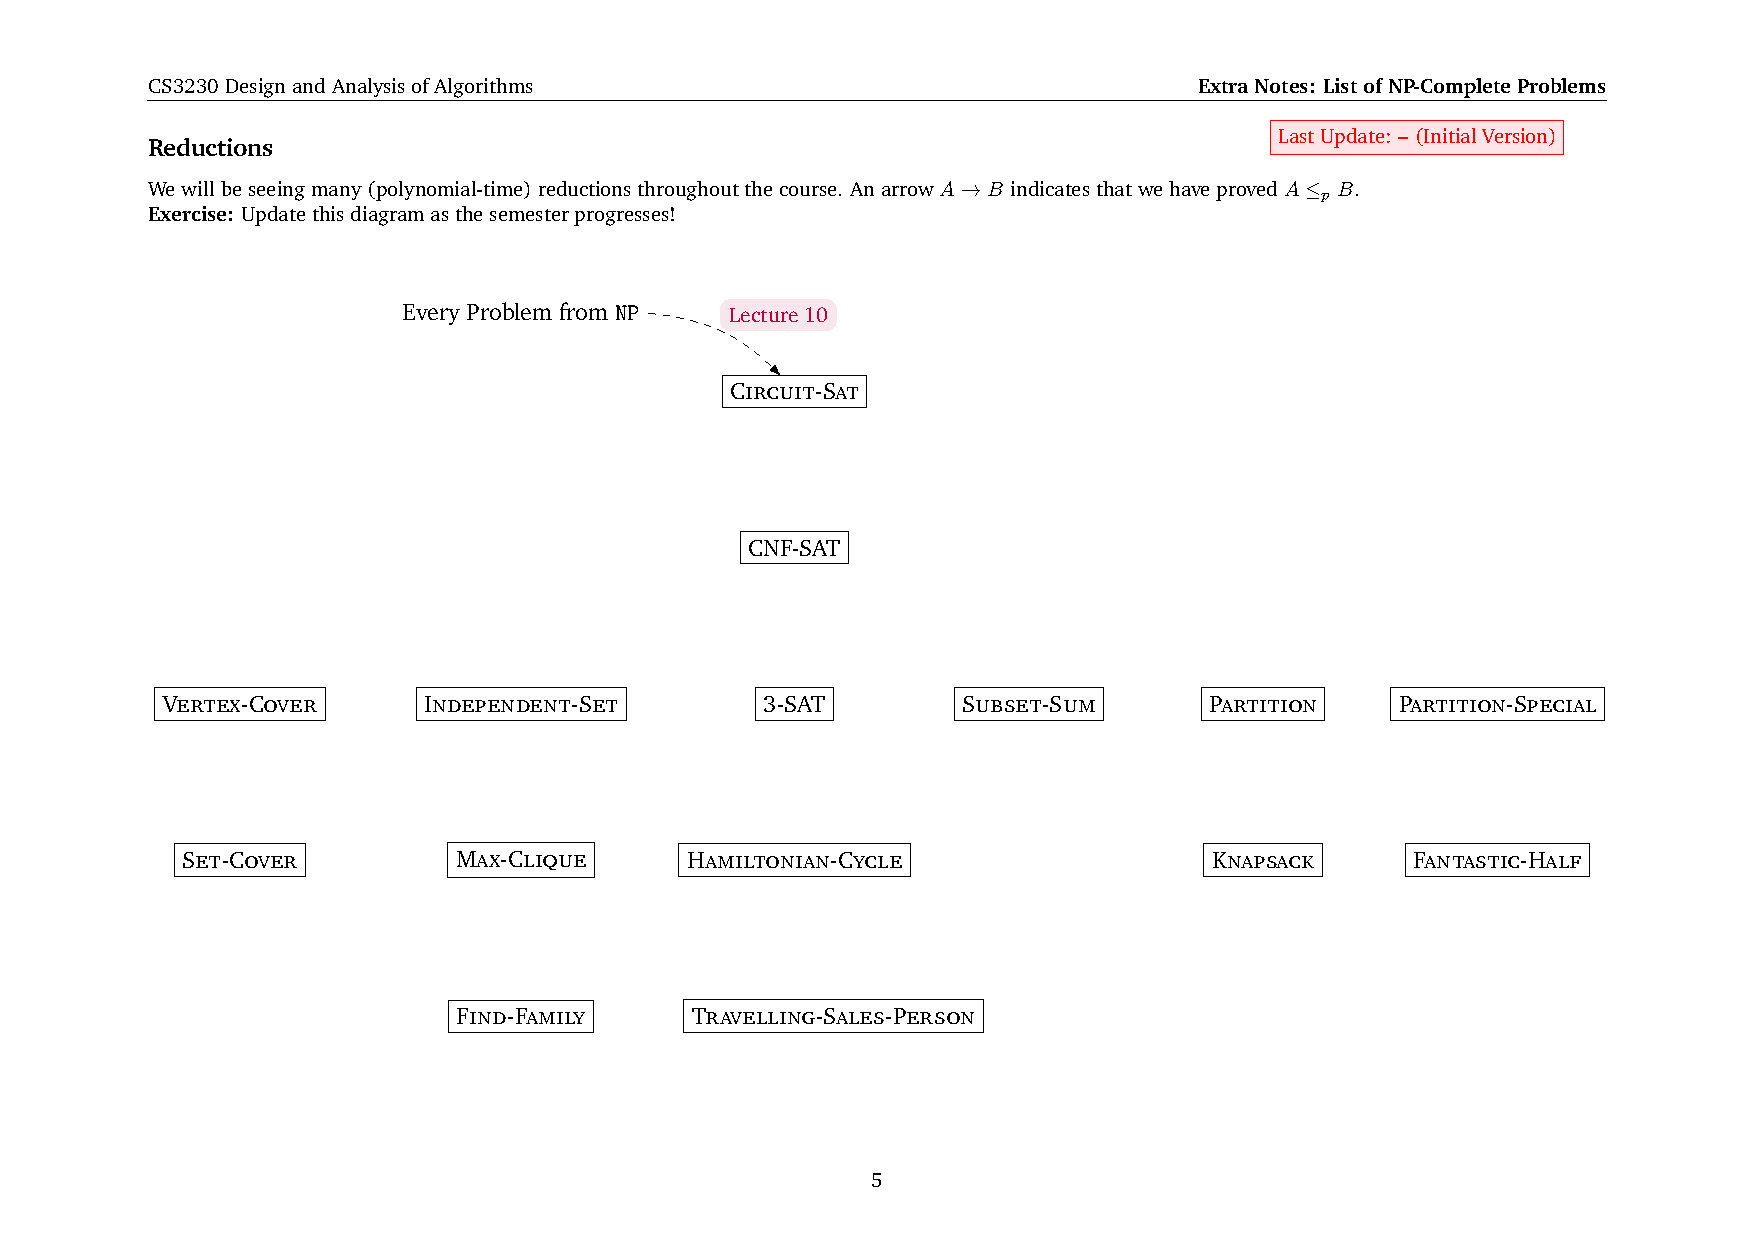
\includegraphics[width=0.85\linewidth]{np-reduction-graph.pdf}
  \caption{Canonical NP-complete reductions covered in this chapter. An arrow $A \to B$ means $A \le_p B$; the dashed arrow from ``Every Problem from \texttt{NP}'' to \textsc{Circuit-Sat} is the Cook--Levin theorem.}
  \label{fig:np_reductions}
\end{figure}

\begin{theorem}[$\textsc{Independent-Set} \le_p \textsc{Clique}$]
\label{thm:is_to_clique}
\textsc{Clique} is $\NP$-complete. The hardness is established by the reduction: given an instance $(G, k)$ of \textsc{Independent-Set} (where $G = (V, E)$), output the instance $(\bar G, k)$ of \textsc{Clique}, where $\bar G = (V, \bar E)$ is the complement graph: $(u, v) \in \bar E$ iff $u \ne v$ and $(u, v) \notin E$.
\end{theorem}

\begin{proof}
\textit{Membership in $\NP$.} A clique $C \subseteq V$ of size $\ge k$ is itself a polynomial-size certificate; the verifier checks $|C| \ge k$ and $(u, v) \in E$ for every distinct pair $u, v \in C$ in $O(k^2)$ time.

\medskip
\noindent\textit{Reduction is polynomial.} Constructing $\bar G$ enumerates all $\binom{|V|}{2}$ pairs and includes them in $\bar E$ iff they are not in $E$, taking $O(|V|^2)$ time.

\medskip
\noindent\textit{($\Rightarrow$).} Suppose $G$ has an independent set $X \subseteq V$ of size $k$. By definition, no two vertices in $X$ are adjacent in $G$, so for every distinct $u, v \in X$ we have $(u, v) \notin E$, hence $(u, v) \in \bar E$. Thus $X$ is a clique of size $k$ in $\bar G$.

\medskip
\noindent\textit{($\Leftarrow$).} Suppose $\bar G$ has a clique $X$ of size $k$. Then for every distinct $u, v \in X$, $(u, v) \in \bar E$, so $(u, v) \notin E$, so $X$ is an independent set of size $k$ in $G$.

\medskip
Since \textsc{Independent-Set} is $\NP$-hard (by reducing $3\textsc{-Sat}$ to \textsc{Independent-Set}; see \cref{sec:reductions}), so is \textsc{Clique}.
\end{proof}

\begin{remark}[Certificates have to translate]
The reduction is correct precisely because the same vertex subset witnesses both sides: a YES-witness $C$ for \textsc{Clique} on $\bar G$ is also a YES-witness for \textsc{Independent-Set} on $G$. Arguing only that ``the optimal value of $A$ on $x$ equals the optimal value of $B$ on $f(x)$'' is necessary but not sufficient for $\le_p$-correctness; one must additionally exhibit a polynomial-time map taking a YES-witness for $f(x)$ back to a YES-witness for $x$.
\end{remark}

\begin{theorem}[$\textsc{Independent-Set} \le_p \textsc{Vertex-Cover}$]
\label{thm:is_to_vc}
\textsc{Vertex-Cover} is $\NP$-complete. The hardness uses the duality: $X \subseteq V$ is a vertex cover of $G = (V, E)$ iff $V \setminus X$ is an independent set of $G$. Reduction: given an instance $(G, k)$ of \textsc{Independent-Set}, output $(G, |V| - k)$ as an instance of \textsc{Vertex-Cover}.
\end{theorem}

\begin{proof}
\textit{$\NP$ membership.} A subset $X \subseteq V$ with $|X| \le k'$ is a certificate; the verifier checks for every edge $(u, v) \in E$ whether $u \in X$ or $v \in X$, in $O(|E|)$ time.

\medskip
\noindent\textit{Reduction is polynomial.} The output is just $(G, |V| - k)$, computed in $O(|V|)$ time.

\medskip
\noindent\textit{Correctness via the duality.} For any $X \subseteq V$, the following are equivalent:
\begin{enumerate}[(i)]
  \item $X$ is a vertex cover, i.e.\ for every edge $(u, v) \in E$, $u \in X$ or $v \in X$;
  \item no edge has both endpoints in $V \setminus X$;
  \item $V \setminus X$ is an independent set.
\end{enumerate}
The first $\iff$ second is contraposition; the second $\iff$ third is the definition of an independent set.

\medskip
\noindent\textit{($\Rightarrow$).} If $G$ has an independent set $Y$ of size $\ge k$, take $X = V \setminus Y$. By the duality, $X$ is a vertex cover; and $|X| = |V| - |Y| \le |V| - k$.

\medskip
\noindent\textit{($\Leftarrow$).} If $G$ has a vertex cover $X$ of size $\le |V| - k$, take $Y = V \setminus X$. By the duality, $Y$ is an independent set; and $|Y| = |V| - |X| \ge k$.
\end{proof}

\begin{corollary}[Three-way equivalence]
\label{cor:is_clique_vc_equivalence}
\textsc{Independent-Set}, \textsc{Clique}, and \textsc{Vertex-Cover} are pairwise polynomial-time equivalent: each reduces to each in polynomial time, via complementation of the graph (\cref{thm:is_to_clique}) and complementation of the vertex set (\cref{thm:is_to_vc}).
\end{corollary}

\begin{theorem}[$3\textsc{-Sat} \le_p \textsc{Directed-Ham-Cycle}$]
\label{thm:3sat_to_dhc}
\textsc{Directed-Ham-Cycle} (and hence \textsc{Hamiltonian-Cycle} on undirected graphs, by a further reduction) is $\NP$-complete. Given a $3$-\textsc{Sat} instance $\Phi$ over variables $x_1, \dots, x_n$ with clauses $C_1, \dots, C_m$, construct a directed graph $G$ as follows.
\begin{itemize}
  \item For each variable $x_i$, build a \emph{horizontal path gadget} $P_i$: a chain of $3m + 3$ vertices with antiparallel edges between consecutive vertices (so the path can be traversed left-to-right or right-to-left). Left-to-right traversal of $P_i$ encodes $x_i = \mathsf{True}$; right-to-left encodes $x_i = \mathsf{False}$.
  \item Add two special vertices $s$ and $t$. Connect $s$ to the left and right ends of $P_1$, and connect both ends of $P_n$ to $t$. Each $P_i$'s endpoints are connected to both endpoints of $P_{i+1}$, so any Hamiltonian cycle traverses the path gadgets one by one, choosing a direction independently for each.
  \item For each clause $C_j = \ell_{j,1} \vee \ell_{j,2} \vee \ell_{j,3}$, add a \emph{clause vertex} $c_j$. For each literal $\ell_{j,k}$, place edges between $c_j$ and a designated pair $(u_{i,j}, v_{i,j})$ of consecutive vertices in $P_i$ (where $i$ is the variable underlying $\ell_{j,k}$): specifically, if $\ell_{j,k} = x_i$, add edge $u_{i,j} \to c_j$ and $c_j \to v_{i,j}$ (so a left-to-right traversal of $P_i$ can ``detour'' through $c_j$); if $\ell_{j,k} = \overline{x_i}$, reverse the orientation. Different clauses use disjoint pairs of consecutive vertices in each $P_i$, which is why each $P_i$ needs $\Theta(m)$ vertices.
\end{itemize}
The output $G$ has $\Theta(nm)$ vertices and edges, constructed in polynomial time.
\end{theorem}

\begin{proof}
\sketchproof
\textit{$\NP$ membership.} A Hamiltonian cycle is itself a polynomial-size certificate; the verifier checks that it visits each vertex exactly once and uses only edges of $G$, in $O(|V|)$ time.

\medskip
\noindent\textit{Reduction is polynomial.} The graph has $\Theta(nm)$ vertices and edges, all constructible in polynomial time.

\medskip
\noindent\textit{($\Rightarrow$).} Suppose $\Phi$ is satisfiable, witnessed by an assignment $\alpha$. Build a Hamiltonian cycle: start at $s$; for each $i = 1, \dots, n$, traverse $P_i$ left-to-right if $\alpha(x_i) = \mathsf{True}$ and right-to-left otherwise. Since $\alpha$ satisfies $\Phi$, each clause $C_j$ contains some literal $\ell_{j,k}$ that is true under $\alpha$; the orientation of $P_i$ (where $i$ is the variable of $\ell_{j,k}$) chosen above is precisely the one that lets the traversal detour through $c_j$ via the dedicated $(u_{i,j}, v_{i,j})$ pair. Pick one such satisfying literal per clause and detour through the corresponding $c_j$; finally connect to $t$ and back to $s$. Each clause vertex is visited exactly once because we detour through exactly one literal per clause.

\medskip
\noindent\textit{($\Leftarrow$).} Suppose $G$ has a Hamiltonian cycle $H$. The key claim (proved by case analysis of the local edges around each clause vertex's two attachment points $u, v$ in $P_i$) is: \emph{after $H$ enters a clause vertex $c_j$ from some $u_{i,j} \in P_i$, it must leave $c_j$ back to the immediately following vertex $v_{i,j}$ in the same $P_i$ -- it cannot ``escape'' to a different $P_{i'}$.} The argument: if $H$ entered $c_j$ from $u$ and exited to a vertex $v'$ in some other path, then the predecessor of the next vertex $v$ in the original $P_i$ would have no remaining valid in-neighbour, leading $H$ to get stuck. Granting the claim, contracting all detours through clause vertices yields a Hamiltonian cycle of the auxiliary graph consisting of just the path gadgets and $s, t$. That cycle must traverse each $P_i$ in a single direction; read off $\alpha(x_i) = \mathsf{True}$ if left-to-right and $\mathsf{False}$ otherwise. Each clause vertex $c_j$ is visited via some literal $\ell_{j,k}$ which (by construction of the detour edges) is true under $\alpha$, so $\alpha$ satisfies every clause, hence $\Phi$.
\end{proof}

\begin{theorem}[$\textsc{Partition-Special} \le_p \textsc{Fantastic-Half}$]
\label{thm:partspec_to_fh}
\textsc{Fantastic-Half} is $\NP$-complete. Recall: \textsc{Partition-Special} asks, given non-negative integers $x_1, \dots, x_n$, whether $\{1, \dots, n\}$ can be partitioned into $I_1 \sqcup I_2$ with $\sum_{i \in I_1} x_i = \sum_{i \in I_2} x_i$ and $|I_1| = |I_2|$; \textsc{Fantastic-Half} asks, given non-negative integer pairs $(a_1, b_1), \dots, (a_n, b_n)$ with $A = \sum a_i$, $B = \sum b_i$, whether some $S \subseteq \{1, \dots, n\}$ with $|S| = n/2$ satisfies $\sum_{i \in S} a_i \ge A/2$ and $\sum_{i \in S} b_i \ge B/2$. Reduction: given $(x_1, \dots, x_n)$, output $a_i := x_i$ and $b_i := X - x_i$ for all $i$, where $X = \sum_i x_i$.
\end{theorem}

\begin{proof}
\textit{$\NP$ membership.} The set $S$ is itself a polynomial-size certificate; the verifier checks $|S| = n/2$, $\sum_{i \in S} a_i \ge A/2$, and $\sum_{i \in S} b_i \ge B/2$ in linear time.

\medskip
\noindent\textit{Reduction validity and runtime.} Each $b_i = X - x_i \ge 0$ since $x_i \le X$, so the constructed instance is valid. The construction takes $O(n)$ time.

\medskip
\noindent\textit{($\Rightarrow$).} If $\{1, \dots, n\}$ partitions into $I_1, I_2$ of equal size and equal sum, take $S = I_1$. Then $|S| = n/2$, and $\sum_{i \in S} a_i = \sum_{i \in S} x_i = X/2 = A/2$. For the $b$-sums, $\sum_{i \in S} b_i = \sum_{i \in S} (X - x_i) = (n/2) X - X/2$, while $B = \sum_i (X - x_i) = nX - X$, so $B/2 = (nX - X)/2 = (n/2) X - X/2$, giving $\sum_{i \in S} b_i = B/2$.

\medskip
\noindent\textit{($\Leftarrow$).} Suppose $S$ satisfies $|S| = n/2$, $\sum_{i \in S} a_i \ge A/2$, and $\sum_{i \in S} b_i \ge B/2$. The first inequality reads $\sum_{i \in S} x_i \ge \sum_{i \notin S} x_i$. The second reads $\sum_{i \in S}(X - x_i) \ge \sum_{i \notin S}(X - x_i)$, i.e.\ $(n/2) X - \sum_{i \in S} x_i \ge (n/2) X - \sum_{i \notin S} x_i$, hence $\sum_{i \in S} x_i \le \sum_{i \notin S} x_i$. The two inequalities together force equality: $\sum_{i \in S} x_i = \sum_{i \notin S} x_i$. So $(I_1, I_2) := (S, \{1, \dots, n\} \setminus S)$ is a valid \textsc{Partition-Special} witness.
\end{proof}

\begin{remark}[Why the obvious reductions $a_i = b_i = x_i$, $b_i = x_{n+1-i}$, and $b_i = -x_i$ all fail]
Three natural attempts fail before the correct reduction $b_i = X - x_i$. The ``copy'' attempt $a_i = b_i = x_i$ breaks ($\Leftarrow$): the inequality $\sum_{i \in S} a_i \ge A/2$ alone is not enough to conclude equality with $\sum_{i \notin S} a_i$ -- the counterexample $(1, 2, 3, 5)$ is a NO-instance of \textsc{Partition-Special} but YES under this map (take $S = \{3, 4\}$ with $a$-sum $8 \ge 11/2$ and $b$-sum $8 \ge 11/2$). The ``reverse'' attempt $b_i = x_{n+1-i}$ permutes but does not negate; the same counterexample still works. The ``negate'' attempt $b_i = -x_i$ \emph{would} force equality (the two reverse inequalities cancel) but violates the non-negativity requirement of \textsc{Fantastic-Half}, producing an invalid instance. Replacing $-x_i$ by $X - x_i$ preserves the cancellation property up to the additive constant $X$ while keeping values non-negative; this is the trick.

The first two failures illustrate that \emph{both directions} of correctness are mandatory: $x \in A \Rightarrow f(x) \in B$ is easy, but the reverse can fail on a small counterexample. The third illustrates that the reduction's output must be a syntactically valid instance of the target -- always check that $f(x)$ satisfies the input constraints of $B$. A separate concern is the runtime bound: the construction must be polynomial in $|x|$, not in the value encoded by $x$. For \textsc{Subset-Sum}-flavour reductions, ``pseudo-polynomial'' time in the magnitude of weights is \emph{not} polynomial time.
\end{remark}

\subsection{Worked example}

\begin{example}[Concrete reduction $\textsc{Independent-Set} \le_p \textsc{Clique}$]
\label{ex:reduction_walkthrough}
Take the small graph $G$ with vertex set $V = \{a, b, x, y, z, t\}$ and edge set
\[
  E = \{(a, b),\ (b, x),\ (x, y),\ (y, t),\ (y, z)\}.
\]
We ask: does $G$ have an independent set of size $\ge 3$? We solve it via the \textsc{Clique} oracle.

\medskip
\noindent\textit{Step 1 -- apply the reduction.} Build $\bar G$ on the same vertex set; an edge $(u, v)$ is in $\bar G$ iff $u \ne v$ and $(u, v) \notin E$. The total number of unordered pairs is $\binom{6}{2} = 15$. Subtracting the $5$ edges of $E$, the complement has $10$ edges:
\[
  \bar E = \{(a,x),\ (a,y),\ (a,z),\ (a,t),\ (b,y),\ (b,z),\ (b,t),\ (x,z),\ (x,t),\ (z,t)\}.
\]

\medskip
\noindent\textit{Step 2 -- ask the target problem.} We ask whether $\bar G$ has a \emph{clique} of size $\ge 3$.

\medskip
\noindent\textit{Step 3 -- inspect.} The triple $\{a, x, t\}$ has all three pairs $(a,x), (a,t), (x,t) \in \bar E$, so it is a clique of size $3$ in $\bar G$. By \cref{thm:is_to_clique} (the $\Leftarrow$ direction), this same triple is an independent set of size $3$ in $G$: indeed, none of $(a,x), (a,t), (x,t)$ is in $E$.

\medskip
\noindent\textit{Step 4 -- certificate translation.} Critically, the reduction's correctness is not just that ``YES corresponds to YES''; it is that the \emph{same set of vertices} is the witness on both sides. A black-box \textsc{Clique} solver returning the clique $\{a, x, t\}$ of $\bar G$ \emph{directly} hands back the desired independent set of $G$. This is the typical structure: the certificate transforms via the same map (or a simple inverse) as the instance itself.

\medskip
\noindent\textit{Polynomial time.} Building $\bar G$ took $O(n^2)$ time. So a hypothetical polynomial-time \textsc{Clique} solver would yield a polynomial-time \textsc{Independent-Set} solver: one $\bar G$-construction followed by one \textsc{Clique} call, then trivially read off the witness.
\end{example}



% --- Appendices ---
\appendix
% Appendix A: Selected Problems.
\section{Selected Problems}
\label{sec:tricky}

\subsection*{How to use this appendix}
Each entry: terse problem statement, the key insight (the ``trick''), and the standard pattern it instantiates.
When a problem of the listed \emph{shape} arises, the listed \emph{trick} applies.

\subsubsection*{Asymptotic analysis}

\subsection{\texorpdfstring{$\log f \in o(\log g)$ does not follow from $f \in o(g)$}{log f in o(log g) does not follow from f in o(g)}}
\textbf{Problem.} If $f \in o(g)$ with both increasing, must $\lceil \log f(n)\rceil \in o(\lceil \log g(n)\rceil)$?\\
\textbf{Trick.} Take $f(n) = 2^n$, $g(n) = 4^n$: $f \in o(g)$ but $\log f = n = \tfrac{1}{2}\log g$. Logs compress exponential gaps to constant factors, breaking little-$o$.\\
\textbf{Pattern.} Big-$O$/$\Theta$ are preserved by logarithms (up to constants), but $o$ and $\omega$ are not. When asked whether an asymptotic relation survives a transformation, check whether the relation tolerates constant multiplicative slack. See \cref{sec:asymptotic}.

\subsubsection*{Recurrences}

\subsection{Recurrence with two unequal recursive calls}
\textbf{Problem.} Solve $T(n) = T(n/2) + T(\sqrt{n}) + 2n$ tightly.\\
\textbf{Trick.} Master theorem does not apply (two recursive calls with different shrink rates). Naive bound $T(n) \leq 2T(n/2) + 2n$ gives $O(n\log n)$, which is loose. Guess $T(n) \leq cn$ and verify by substitution: the $\sqrt{n}$ branch contributes only $c\sqrt{n} \leq (c-4)n/2$ for $n \geq 10$ with $c \geq 12$. So $T(n) \in \Theta(n)$.\\
\textbf{Pattern.} When master theorem fails, try the substitution method with a linear (or otherwise sharp) guess; the $\sqrt{n}$ subproblem is asymptotically negligible compared to $T(n/2) + n$. See \cref{sec:recurrences}.

\subsubsection*{Divide and conquer}

\subsection{H-index by unbounded (galloping) binary search}
\textbf{Problem.} Given a non-increasing array $A[1..n]$, find the largest $i$ with $A[i] \geq i$ (the H-index).\\
\textbf{Trick.} The plain binary search costs $O(\log n)$ regardless of where the answer lies. To get $O(\log H)$ when the H-index $H$ is small, first \emph{gallop}: probe $i = 1, 2, 4, \ldots, 2^k$ until $A[2^k] < 2^k$, then binary-search inside $[2^{k-1}, 2^k]$. Total: $O(\log H)$.\\
\textbf{Pattern.} ``Output-sensitive search'': when the answer might be much smaller than $n$, exponentially expand the search range before binary-searching. Same idea as searching in an unbounded sorted stream. See \cref{sec:dnc}.

\subsection{Two-scanner search with a moving target}
\textbf{Problem.} A fighter hides in one of $n$ bunkers; two scanners may be queried once per day at 6\,AM (each tests an interval); after each scan, the fighter may move to an adjacent bunker. Minimise the number of days.\\
\textbf{Trick.} With two simultaneous interval scanners, you can quarter the uncertainty per day (four outcome patterns), giving $\log_4 n$ days statically. The mobility adds at most $+2$ to the interval each night, so the recurrence becomes $u_{d+1} \leq u_d/4 + 2$, whose fixed-point is constant; $\lceil \log_4 n\rceil + O(1)$ days still suffice.\\
\textbf{Pattern.} $k$ parallel binary tests divide the search space by $k+1$, not by~2. With perturbations between rounds, set up a recurrence whose dominant term is the $1/(k+1)$ shrink and absorb the additive perturbation as a geometric tail. See \cref{sec:dnc}.

\subsubsection*{Sorting and lower bounds}

\subsection{\texorpdfstring{Sorting pairs $(x,y)$ by $x + n^y$ in $O(n)$}{Sorting pairs (x,y) by x+n\^{}y in O(n)}}
\textbf{Problem.} Sort $n$ pairs $(x_i, y_i)$ with $1 \leq x_i, y_i < n^3$ by $\mathrm{val}(x,y) = x + n^y$ in $O(n)$ time.\\
\textbf{Trick.} The $\Omega(n\log n)$ comparison lower bound does not apply because we can read digits, so radix sort is fair game. \emph{Splitting on $y$ is essential}: when $y_j > 3$, $n^{y_j}$ dominates $x_j$; for $y \leq 3$, $\mathrm{val}$ fits in $2n^3$ and a single radix sort works. Otherwise, two passes (radix-sort by $x$, then stable radix-sort by $y$) finish the rest. Each pass is $O(n)$ since values are $\le n^3$ (constant number of digits in base $n$).\\
\textbf{Pattern.} When values are polynomial in $n$, view them as $O(1)$-digit base-$n$ numbers and apply radix sort for $O(n)$ sorting. Beware mixing scales: split the input into ``small'' and ``large'' regimes when one component dominates the other. See \cref{sec:sorting}.

\subsubsection*{Randomised algorithms}

\subsection{Existence proofs via the probabilistic method}
\textbf{Problem.} Show every graph has an independent set of size at least $\sum_{v} \frac{1}{d(v)+1}$.\\
\textbf{Trick.} Pick a uniform random vertex order; let $I$ contain each $v$ all of whose neighbours come after it. $I$ is independent by construction. By linearity of expectation, $\Pr[v \in I] = \frac{1}{d(v)+1}$, so $\expec[|I|] = \sum_v \frac{1}{d(v)+1}$. Some realisation must achieve at least the expectation.\\
\textbf{Pattern.} \emph{Probabilistic method}: to prove existence of a structure of size $\geq L$, design a random construction whose expectation is $L$. Indicator + linearity of expectation does the heavy lifting; conditional independence is not needed. See \cref{sec:randomised}.

\subsubsection*{Dynamic programming}

\subsection{\texorpdfstring{Minimise $|S_X - 2 S_Y|$ via subset-sum DP}{Minimise |S\_X - 2 S\_Y| via subset-sum DP}}
\textbf{Problem.} Partition indices into $X, Y$ minimising $|\sum_{X} A[i] - 2\sum_{Y} A[i]|$, where $0 \le A[i] \le M$.\\
\textbf{Trick.} Let $S = \sum A[i]$ and $t = \sum_Y A[i]$. Then the objective rewrites as $|S - 3t|$. So we just need a subset-sum closest to $S/3$: a standard pseudo-polynomial $O(nS) = O(n^2 M)$ DP table, then scan for the best feasible $t$.\\
\textbf{Pattern.} Algebraically reduce a multi-set objective to a single-variable one (here, the target sum $t$); then the problem becomes a known DP. The space of achievable subset sums is the canonical reduction target. See \cref{sec:dp}.

\subsubsection*{Greedy algorithms}

\subsection{Interval cover: pick the latest finish among feasible starts}
\textbf{Problem.} Cover days $1..M$ with the fewest guard intervals $[a_i, b_i]$.\\
\textbf{Trick.} Sweep: maintain frontier $m$ (next uncovered day, initially~$1$). Among guards with $a_i \leq m$, pick the one with the largest $b_i$, then advance $m \leftarrow b_i + 1$. Exchange argument: any optimal solution must include some guard active on day~$m$; swap that guard for the latest-finishing such guard without losing feasibility.\\
\textbf{Pattern.} \emph{Greedy choice with exchange argument}: identify a structural ``pinch point'' (here, day~$m$ must be covered \emph{somehow}), then show the most aggressive feasible choice at that point is safe. Compare to activity selection. Note: this stops being greedy once weights enter (a weighted variant requires DP). See \cref{sec:greedy}.

\subsubsection*{Amortised analysis}

\subsection{Repeated set unions cost \texorpdfstring{$O(n \log n)$}{O(n log n)}}
\textbf{Problem.} Start with $n$ singletons. Repeatedly union two sets at cost $\min(|A|,|B|)$ until one set remains. Show total cost $\leq \tfrac{n}{2} \log n$ regardless of strategy.\\
\textbf{Trick.} Charge to elements, not operations. Define $\phi_i = \log|S(i)|$ where $S(i)$ is element $i$'s current set. Merging sets of sizes $a \geq b$: each element on the small side gains $\log\frac{a+b}{b} \geq \log 2 = 1$, each on the large side gains $\log(1 + b/a) \geq b/a$. Summing: total potential rises by $\geq 2b$, twice the cost. Since $\phi_i \in [0, \log n]$, the total potential is at most $n \log n$, giving cost $\leq \tfrac{n}{2}\log n$.\\
\textbf{Pattern.} \emph{Potential per element} (not per operation) is the right granularity for size-based merge costs. The estimate $\log(1+x) \geq x$ for $x \in [0,1]$ converts a logarithmic potential change into a linear lower bound, matching the merge cost. Same scheme as weighted-union-find analysis. See \cref{sec:amortised}.

\subsubsection*{Reductions and NP-completeness}

\subsection{Decision-to-search via self-reduction (Hamiltonian cycle, 3-SAT)}
\textbf{Problem.} Given a polynomial-time \emph{decider} for Hamiltonian cycle (resp.\ 3-SAT), find an actual Hamiltonian cycle (resp.\ a satisfying assignment) in polynomial time.\\
\textbf{Trick.} Iteratively commit and re-test. For HC: at each vertex, try keeping one outgoing edge and deleting the rest; if the decider still says YES, commit. For 3-SAT: set $x_1 \!=\! 1$, ask the decider; if YES, fix it, else set $x_1 \!=\! 0$; repeat for $x_2, \ldots, x_n$. Each commit preserves the YES-instance invariant, and only $\mathrm{poly}(n)$ decider calls are made.\\
\textbf{Pattern.} \emph{Self-reduction}: when the search problem and the decision problem share the structure ``A solution exists in $G$ iff a solution exists in $G$ restricted by one bit'', reduce search to a polynomial sequence of decisions. This is why search and decision are polynomially equivalent for NP-complete problems. See \cref{sec:reductions}, \cref{sec:npc}.

\subsection{Reducing CLIQUE to Half Clique by padding}
\textbf{Problem.} Show Half Clique (does $G$ on $|V|$ vertices have a clique of size exactly $|V|/2$?) is NP-complete.\\
\textbf{Trick.} The size constraint is rigid. From $(\hat G, k)$ with $|V(\hat G)| = n$, build $G$ by adding $n-k$ new vertices forming a clique fully connected to $\hat G$, plus $k$ isolated vertices. Total $2n$ vertices; a clique of size $n$ exists iff $\hat G$ has a $k$-clique.\\
\textbf{Pattern.} \emph{Padding reductions}: when the target problem fixes a size to half (or another constant fraction) of $|V|$, add cliques to ``promote'' a small clique and isolated vertices to control the vertex count. Same flavour as reducing one fixed-size variant to another. See \cref{sec:npc}.


% Appendix B: alphabetical index of definitions
\printindex

% Appendix C: list of theorems and lemmas
\newpage
\listoftheorems[ignoreall, show={theorem,lemma,corollary,proposition}]

\end{document}
